\documentclass[letterpaper,oneside,11pt]{report}
% Package loading---------------------------------
\usepackage{fitthesis}
\usepackage{epsfig}
\usepackage{graphicx}

% \usepackage[ruled,vlined,linesnumbered]{algorithm2e}
\usepackage{algpseudocodex}
\usepackage{algorithm}
\usepackage{setspace}
\usepackage{tabularx}
\usepackage{hyperref}
\usepackage[a-1b]{pdfx}
\usepackage{biblatex}
\addbibresource{mybibliography.bib}

\usepackage{caption}
\usepackage{subcaption}
% \usepackage{subfig}
% \usepackage[subfigure]{tocloft} % no number for Vita in ToC
\usepackage{fancyhdr}
\usepackage[english]{babel}
\usepackage{footmisc}
% \usepackage{algorithmic}
\usepackage{listings}
\usepackage{fancyvrb}
\usepackage{booktabs}
\usepackage{epstopdf}

\usepackage[]{pdflscape}
\usepackage[]{longtable}
\usepackage{multirow}
\usepackage{xcolor}
\usepackage{colortbl}

\usepackage{pdfpages}

\usepackage{amsmath}
% \usepackage{gensymb}

\graphicspath{{images/}}  % Location of the graphics files

% Set colors
\definecolor{dkgreen}{rgb}{0,0.6,0}
\definecolor{gray}{rgb}{0.5,0.5,0.5}
\definecolor{mauve}{rgb}{0.58,0,0.82}
\definecolor{verifiedGreen}{rgb}{99, 190, 123}
\definecolor{verifiedRed}{rgb}{248, 105, 107}

% Set code styles
\lstdefinestyle{customBashStyle}{
	frame=shadowbox,
	language=bash,
	aboveskip=6mm,
	belowskip=3mm,
	showstringspaces=false,
	columns=flexible,
	basicstyle={\footnotesize\ttfamily},
	numbers=none,
	numberstyle=\tiny\color{gray},
	keywordstyle=\color{blue},
	commentstyle=\color{dkgreen},
	stringstyle=\color{mauve},
	breaklines=true,
	breakatwhitespace=true,
	tabsize=3
}

\lstdefinestyle{customInline}{
	basicstyle={\normalsize\ttfamily},
	numbers=none,
	numberstyle=\normalsize\color{gray},
	keywordstyle=\color{blue},
	commentstyle=\color{dkgreen},
	stringstyle=\color{mauve}
}

\lstnewenvironment{bash}
{
	\lstset{
		style=customBashStyle	
	}
}
{}


% To get single-space, (for drafts only!) use:
% \singlespacing

% To consistently get dotted lines in the Table of Contents
\makeatletter
\renewcommand*\l@part[2]{%
	\ifnum \c@tocdepth >-2\relax
	\addpenalty{-\@highpenalty}%
	\addvspace{2.25em \@plus\p@}%
	\setlength\@tempdima{3em}%
	\begingroup
	\parindent \z@ \rightskip \@pnumwidth
	\parfillskip -\@pnumwidth
	{\leavevmode
		\large \bfseries #1\nobreak\normalfont\leaders\hbox{$\m@th
			\mkern \@dotsep mu\hbox{.}\mkern \@dotsep
			mu$}\hfill\nobreak \hb@xt@\@pnumwidth{\hss #2}}\par
	\nobreak
	\global\@nobreaktrue
	\everypar{\global\@nobreakfalse\everypar{}}%
	\endgroup
	\fi}
\renewcommand*\l@chapter[2]{%
	\ifnum \c@tocdepth >\m@ne
	\addpenalty{-\@highpenalty}%
	\vskip 1.0em \@plus\p@
	\setlength\@tempdima{1.5em}%
	\begingroup
	\parindent \z@ \rightskip \@pnumwidth
	\parfillskip -\@pnumwidth
	\leavevmode \bfseries
	\advance\leftskip\@tempdima
	\hskip -\leftskip
	#1\nobreak\normalfont\leaders\hbox{$\m@th
		\mkern \@dotsep mu\hbox{.}\mkern \@dotsep
		mu$}\hfill\nobreak\hb@xt@\@pnumwidth{\hss #2}\par
	\penalty\@highpenalty
	\endgroup
	\fi}
\makeatother

% Label commands
\newcommand{\labchap}[1]{\label{chap:#1}}
\newcommand{\labsec}[1]{\label{sec:#1}}
\newcommand{\labsubsec}[1]{\label{ssec:#1}}
\newcommand{\labfig}[1]{\label{fig:#1}}
\newcommand{\labsubfig}[1]{\label{subfig:#1}}
\newcommand{\labtab}[1]{\label{tab:#1}}
\newcommand{\labeq}[1]{\label{eq:#1}}

% Revision figure command
\newcommand{\revisionfigure}[1]{
    \begin{figure}[H]
		\labfig{thetis_rev_#1}
        \caption{Thetis Revision \uppercase{#1} PCB render with call outs for important components.}
		\centering
		\includegraphics[width=5in]{design/revision_#1_labeled.png}
    \end{figure}
}

% Include schematic command
\newcommand{\schematic}[1]{
	\includepdf[landscape=true, width=\textheight, offset=-0in -0.25in, pagecommand={\subsection{Revision #1 Schematic} \labsubsec{rev#1_schematic}}]{../include/Thetis_Rev#1_SCH.pdf}
}


\title{Project Thetis\\ A Low-Cost, Low-Profile Inertial Datalogger}
\author{Braidan Duffy}

% \GradDocumentType can be of the following: thesis, dissertation, design project, doctoral research project
\GradDocumentType{thesis}

% Change this to be the college or school you are part of. For Example \CollegeOrSchoolName{College of Engineering and Science}
\CollegeOrSchoolName{College of Engineering and Sciences}

% Degree you are applying for, defaults to Master of Engineering
\degree{Masters of Science}
\dept{Ocean Engineering}

% Your Previous Degree \\ University, year
\authordegree{Bachelor of Science \\Ocean Engineering\\ Florida Institute of Technology\\ 2021}
% Month and Year document is turned in or graduation
\copyrightmonth{December}
\copyrightyear{2023}

% Define Committee Information
\directorname{Dr. Stephen Wood, Ph.D., P.E.}
\directortitle{Program Chair}
\directordept{Ocean Engineering and Marine Sciences}

% Third Committee Member
\secondreadername{Dr. Hector Gutierrez, Ph. D., P.E.}
\secondreadertitle{Professor}
\secondreaderdept{Mechanical Engineering}

% Second Committee Member / Outside Member
\thirdreadername{Dr. Robert Weaver, Ph. D}
\thirdreadertitle{Associate Proffesor}
\thirdreaderdept{Ocean Engineering and Marine Sciences}

% Forth Committee Member
\toggletrue{useforthreader}
\forthreadername{Dr. Marius Silaghi, Ph.D.}
\forthreadertitle{Professor}
\forthreaderdept{Comupter Engineering and Sciences}

% Use Academic Unit Head
\toggletrue{useacademicunithead}
\academicunitheadname{Dr. Richard Aronson, Ph.D.}
\academicunitheadtitle{Department Head}
\academicunitheaddept{Ocean Engineering and Marine Sciences}


% The following page is optional, to disable please use \togglefalse{usecopyrightpage}
\toggletrue{usecopyrightpage}

\begin{document}
	
	% For MS students
	\makethesistitle

	
	% This abstract maintains the same look as all other sections.
	% Include Abstract Text
	%%-------------Abstract-----------------
% Length:Ideally, one page or less
% Ph.D. Dissertations: 350 word maximum.
\abstract{
This thesis details the design, testing, calibration, and verification of a nine degree of freedom inertial measurement data logger for use with floating bodies.
The instrument was conceived to address limitations of equipment used in classes within the Ocean Engineering department at Florida Institute of Technology.
By meeting with several stakeholders and end users, a series of stakeholder requirements, capabilities, and component-level requirements were developed that informed the design constraints.
There were several hardware iterations of the board, culminating in Revision F5 which was extensively tested and proven.
The design was inspected after testing concluded to determine which capabilities or requirements were met and detail additional efforts for future students.
Overall, the design was successful and promises to be a compelling instrument for use in class and laboratory environments.
With some additional work, it may become more equivalent to some of its commercial counterparts.
}
	\makeumiabstract
	
	\pagebreak
	% Optional
	% \prefacesection{Preface}
	\setcounter{secnumdepth}{6}
	\setcounter{tocdepth}{4}
	\newpage
	\maketableofcontents
	% \listoftables
	% \newpage
	\makelistoffigures
	%Uncomment following line if you have 4 or more tables
	% \newpage
	\makelistoftables
	
%% -----------Abbreviations-------------------------
%%-----------List of Symbols, Nomenclature or Abbreviation--------
\chapter*{List of Symbols, Nomenclature or
Abbreviations} \addcontentsline{toc}{chapter}{Abbreviations}

\begin{longtable}{l m{0.3\textwidth} m{0.5\textwidth}}
    % \renewcommand{\arraystretch}{1.5} % Set row height
    % \begin{tabular}{l m{0.3\textwidth} m{0.5\textwidth}}
        Symbol & Meaning & Definition \\
        \hline
        $\phi$ & Roll & Typically, any rotation about the center or longitudinal (x) axis \\
        $\theta$ & Pitch & Typically, any rotation about the side or transverse (y) axis \\
        $\psi$ & Yaw & Typically, any rotation about the vertical (z) axis \\
        MEMS & Microelectromechanical Systems & Small electromechanical systems that perform a function and are micrometers in size \\
        MARG & Magnetic, Angular Rate, and Gravity & A collection of tri-axial magnetometers, gyroscopes, and accelerometers in a sensor package \\
        IMU & Inertial Measurement Unit & A collection of gyroscopes and/or accelerometers (optionally with magnetometers) in a sensor package \\
        DOF & Degree(s) of Freedom & A measurement or movement axis in a body \\
        GPS & Global Positioning System & A collection of satellites in Earth orbit that allows receivers to triangulate their position \\
        ToF & Time of Flight & The time it takes a signal (typically electromagnetic) to be emitted, reflected, and return back to the emitter \\
        AHRS & Attitude and Heading Reference System & An algorithm (or collection of algorithms) that report body attitude and heading from sensor data \\
        VCS & Version Control Software & Software that tracks changes made to files and keeps a detailed history \\
        SWaP & Size, Weight, and Power & Three of the most important metrics for considering the design of an embedded system \\
        SCWaP & Size, Cost, Weight, and Power & Four of the most important metrics for considering the design of an embedded system \\
        COTS & Commercial Off The Shelf & Components that can be routinely purchased from stores, retailers, suppliers, catalogs, etc. \\
        API & Application Program Interface & A protocol that allows for standard interactions between different software packages \\
        PCB & Printed Circuit Board & A (typically) fiberglass substrate with etched copper planes that condense electronics designs \\
        IC & Integrated Circuit & A circuit that is integrated into a small board mountable package \\
        DDS & Distributed Data Service & A method for sending messages between different software packages \\
        ROS & Robot Operating System & A framework for handling DDS interactions between nodes in a software package \\
        HAT & Hardware Attached on Top & A daughter board that can be attached onto a Raspberry Pi mini computer to expand its capability
    % \end{tabular}
\end{longtable}


%% -----------Acknowledgments-----------------------
%%-----------Acknowledgements---------------
\chapter*{Acknowledgements}
\addcontentsline{toc}{chapter}{Acknowledgments} Here are your acknowledgments! Don't forget to thank your sponsor

%% -----------Dedication----------------------------
%% -----------Dedication----------------
\chapter*{Dedication}
\addcontentsline{toc}{chapter}{Dedication} Here is your dedication!
Lorem ipsum dolor sit amet, idque apeirian mnesarchum vix ea, usu no mandamus constituam comprehensam, cum cu vero definitionem. Fabulas probatus ne pro, eleifend hendrerit adipiscing at vim. Usu eu facilisis persecuti. Ne has vidit principes efficiantur, has liber euripidis no. Vide sapientem salutandi per at. Eu probo democritum referrentur pri, an vidit simul reprimique nam. Omnium eruditi ex per, elit regione reprimique te eos. Dicam timeam no nam. Tacimates indoctum inciderint ad his, sea fastidii appetere oporteat an. Ad cum movet efficiantur. Sale labitur no vis, complectitur consequuntur usu te. Mel te putant timeam denique. Ne mel vidit ancillae. Ius saperet facilisi an. Eligendi scaevola sea ex, ad recteque cotidieque quo. Te sumo brute eum.

%% -----------change single space to double space---
\doublespacing \pagenumbering{arabic}

%% -----------Main Matter---------------------------
%%-----------Chapters start-------------------------------------
%%-----------Chapter 1------------------------------------------
\chapter{Introduction}\label{chap:intro}
Lorem ipsum dolor sit amet, et has commodo habemus, mel euismod laoreet an. Ignota euripidis te qui, impedit minimum eos id. Ne mundi theophrastus vim, in admodum inimicus mei. Mei viris viderer facilisi ne. Brute mucius causae sit at. Ius vero epicuri assueverit te, tale liber timeam vel ne.

Ex quo oblique denique. Summo eligendi expetenda duo id. No facer adversarium est, eu dictas malorum blandit per. Eu harum petentium qui. Has blandit persequeris appellantur ei, est id detraxit quaerendum. Gubergren persequeris duo cu. An est tempor discere, suavitate vituperatoribus ea nec.

Nullam repudiandae ex his, ad vix probo sonet primis. Sit porro saperet incorrupte eu, quas numquam vivendum mea ei. Vim tollit deleniti ea, vix probatus scriptorem in. Labitur fabellas has et. Pri prima clita no, his animal efficiantur ei.

Vix dico sonet albucius ne. Cu dicat exerci molestiae quo. Mel id utroque copiosae, omnis noluisse eum in. Eum singulis sadipscing persequeris ad, te soluta equidem propriae his, his affert complectitur et. Iriure definitiones usu te.

Clita vivendo argumentum eu mea, his et error maiorum noluisse. Vis te debet eligendi. Ea odio maiorum philosophia vis. Ne vis essent feugait, nonumy ceteros persecuti cu usu. Vel ex modus voluptua, commodo offendit ad sea.
%%----------Chapter 2------------------------------------------
\chapter{How  It Works}\label{chap:background}
Measuring the movement of bodies in three dimensional space is not a new field of study.
Especially in our current age of electronics, one can simply grab an accelerometer and microcontroller off of the Internet, have it delivered in less than 96 hours, and know the accelerations felt on a roller coaster or be able to orient a 3D rendering of a bunny \footnote[1]{https://learn.adafruit.com/adafruit-bno055-absolute-orientation-sensor/overview}.
What makes today exciting is that improvements in manufacturing and computational density have drastically increased the capabilities of small embedded systems.
Now, every cell phone has a sophisticated suite of sensors built into them that have the simple task of detecting whether the phone is in a landscape or portrait mode. 
Some applications, like Google Maps, have gone further and fused the sensor data, along with GPS information and computer vision, into a robust pedestrian navigation system \footnote[2]{https://gizmodo.com/i-tried-google-maps-experimental-walking-directions-of-1833225629}.

\section{Orientation and Rotation} \label{sec:bkg_orientation}
A body can be rotated in 3D space along the x-, y-, and z-axis.
\textbf{Roll ($\phi$)} defines rotation about the x-axis; \textbf{pitch ($\theta$)} defines rotation about the y-axis; and \textbf{yaw ($\psi$)} defines rotation about the z-axis.
These three rotations are known as Euler angles.

A body's orientation is always relative to another coordinate frame.
Consider a person standing straight and still on the Earth's surface.
Each of their appendages could be considered at some orientation relative to their body.
At rest and in their local coordinate frame, the person's body may not be considered moving or rotating.
But, when the scope is expanded to encompass the entire body and the Earth's frame, that person is now rotating about the Earth coordinate frame at almost 17,000 MPH.

\begin{figure}[h!]
    \caption[Body rotations]{Basic look at a 3D body and the axes of rotation in the body reference frame.}
    \label{fig:body_rotations}
    \centering
    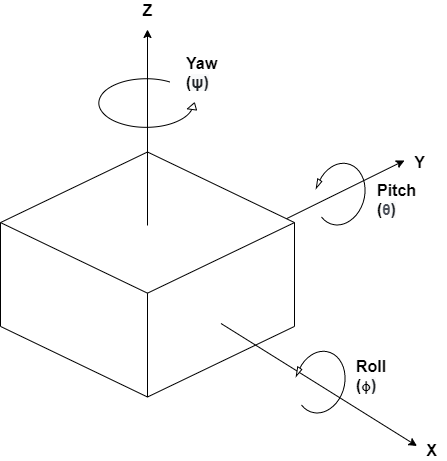
\includegraphics[height=2.5in]{background/body_rotations.png}
\end{figure}

\begin{figure}
    \begin{fitbox}[frametitle=Aside: Notation and Nomenclature for Rotations]
        Bodies on their own typically use the "X, Y, Z" notation that is ubiquitous for the Cartesian coordinate system.
        However, when refering to planetary bodies like the Earth, this nomenclature typically changes to North, East, and Down (NED).
        This occurs because on the surface of a large spherical body, we can assume the local area is a plane tangential to the surface.
        To keep the broader scope in mind, we arbitrarily associate the X-axis with East, the Y-axis with North, and the Z-axis with Down towards the Earth's core (perpendicular to the surface).

        [TODO: INSERT GRAPHIC ON BODY AND PLANET COORDINATE FRAME]
    \end{fitbox}
\end{figure}

\subsection{Rotation Matrices}
A rotation matrix is a mathematical model for translating one body's inertial reference frame to another, e.g. local body to the global body.
These are used for Eulerian transformations of vectors.
The matrix is an $N \times N$ orthogonal matrix where $N$ is the number of dimensions in the vector;
for a three dimensional vector, the rotation matrix to go from one coordinate frame to another would be a $3 \times 3$ matrix.

[TODO: INSERT FIGURE ON FRAME ROTATIONS]

In Figure \ref{fig:frame_rotation}, we can see a base coordinate frame, $A$, and a different coordinate frame, $B$ that is rotated relative to the base frame about the axis, $\vec{r}$.
To express the rotation from the base to the local frame, we can borrow notation from Craig [CITE - Introduction to Robotics].
The "from" or "base" frame is the preceding superscript while the "to" or "local" frame is the preceding subscript, as shown below:

\begin{equation*}
    {}^A_B R = \left[
        \begin{matrix}
            r_{11} & r_{12} & r_{13} \\
            r_{21} & r_{22} & r_{23} \\
            r_{31} & r_{32} & r_{33}
        \end{matrix}
    \right] = \left[
        \begin{matrix}
            {}^Ax_b & {}^Ay_B & {}^Az_B
        \end{matrix}\right]
\end{equation*}

When we want to rotate a vector between frames, we must choose an order in which to do so.
For example, if we wanted to rotate from frame $A$ to frame $B$ using a yaw-pitch-roll rotation order, we can construct the following rotation matrix from Appendix \ref{sec:3d_rot_mat}:

\begin{align*}
    {}^A_B R = R_z(\psi) R_y(\theta) R_x(\phi) &= \left[
        \begin{matrix}
            \cos\psi & -\sin\psi & 0 \\
            \sin\psi & \cos\psi & 0 \\
            0 & 0 & 1
        \end{matrix}\right]
        \left[\begin{matrix}
            \cos\theta & 0 & \sin\theta \\
            0 & 1 & 0 \\
            -\sin\theta & 0 & \cos\theta
        \end{matrix}\right]
        \left[\begin{matrix}
            1 & 0 & 0 \\
            0 & \cos\phi & -\sin\phi \\
            0 & \sin\phi & \cos\phi 
        \end{matrix}\right] \\ \\
        &= \left[\begin{matrix}
            \cos\psi\cos\theta & \cos\psi\sin\theta\sin\phi-\sin\psi\cos\theta & \cos\psi\sin\theta\cos\phi+\sin\psi\sin\phi \\
            \sin\psi\cos\theta & \sin\psi\sin\theta\sin\phi+\cos\psi\cos\phi & \sin\psi\sin\theta\cos\phi-\cos\psi\sin\phi \\
            -\sin\theta & \cos\theta\sin\phi & \cos\theta\cos\phi
        \end{matrix}\right]
\end{align*}

Then, we can rotate the vector from $A$ to $B$ via:

\begin{equation*}
    {}^A\vec{v}_B = {}^A_B R \cdot \vec{v}_A
\end{equation*}

\paragraph*{Gimbal Lock} \label{par:gimbal_lock}
When two axes become parallel, Eulerian changes to either axis become irrelevant, ergo, the system loses a degree of freedom.
This condition is called "gimbal lock".
When in gimbal lock, rotations yield discontinuities that need to be mitigated by changing the rotation order, or moving two or three axes at once.
This can create strange pathways for the body and cause unexpected behavior.
Monitoring for and breaking gimbal lock are also computationally expensive as the program must perform multiple matrix multiplications and then have logic to determine if a) it is in a gimbal lock condition and b) what rotation order would be required to break the condition.

The figure below shows a body's rotation while in gimbal lock. The rotation order is roll-pitch-yaw.
First, it is pitched 90 degrees upwards to align the roll and yaw axes, $\langle0, 90, 0\rangle$ (Figure \ref{subfig:ship_009000}).
If we then want it's orientation to be $\langle90, 0, 0\rangle$ (Figure \ref{subfig:ship_900000}), the body would be rolled left 90 degrees and pitched down 90 degrees.
However, due to gimbal lock, the body ended up in the orientation $\langle0, 0, 90\rangle$ (Figure \ref{subfig:ship_000090})!
To break the gimbal lock and get to the correct orientation, the rotation order would have to be changed to pitch-yaw-roll, or the roll and yaw axes driven simultaneously.

\begin{figure}[h!]
    \centering
    \subfloat[Start: $\langle0, 0, 0\rangle$]{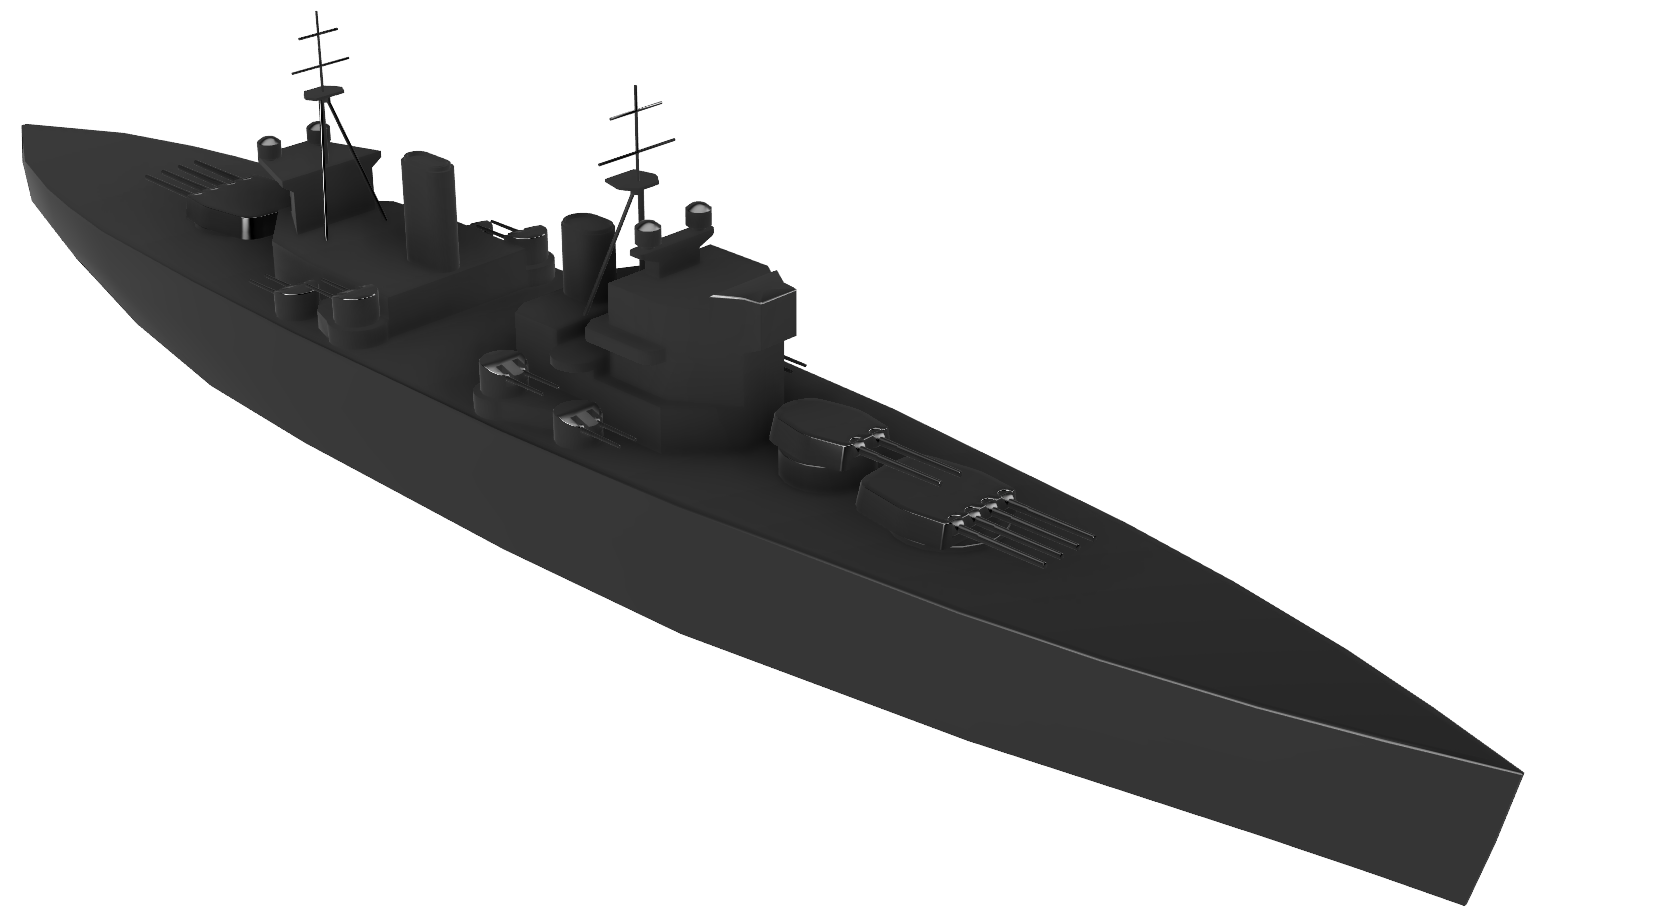
\includegraphics[width=0.25\textwidth]{background/ship_000000}\label{subfig:ship_000000}}\hskip3ex
    \subfloat[$\langle0, 90, 0\rangle$]{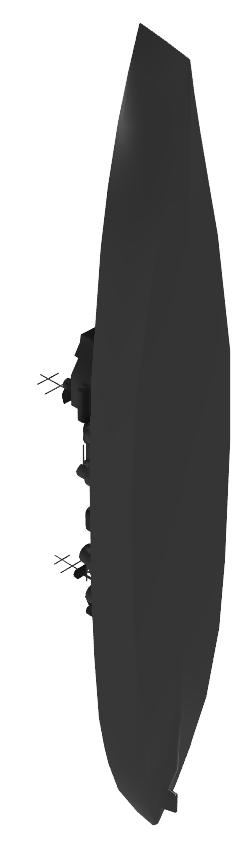
\includegraphics[height=1in]{background/ship_009000}\label{subfig:ship_009000}}\hskip10ex
    \subfloat[$\langle90, 90, 0\rangle$]{
\includegraphics[height=1in]{background/ship_909000}\label{subfig:ship_909000}}\hskip5ex
    \subfloat[End: $\langle0, 0, 90\rangle$]{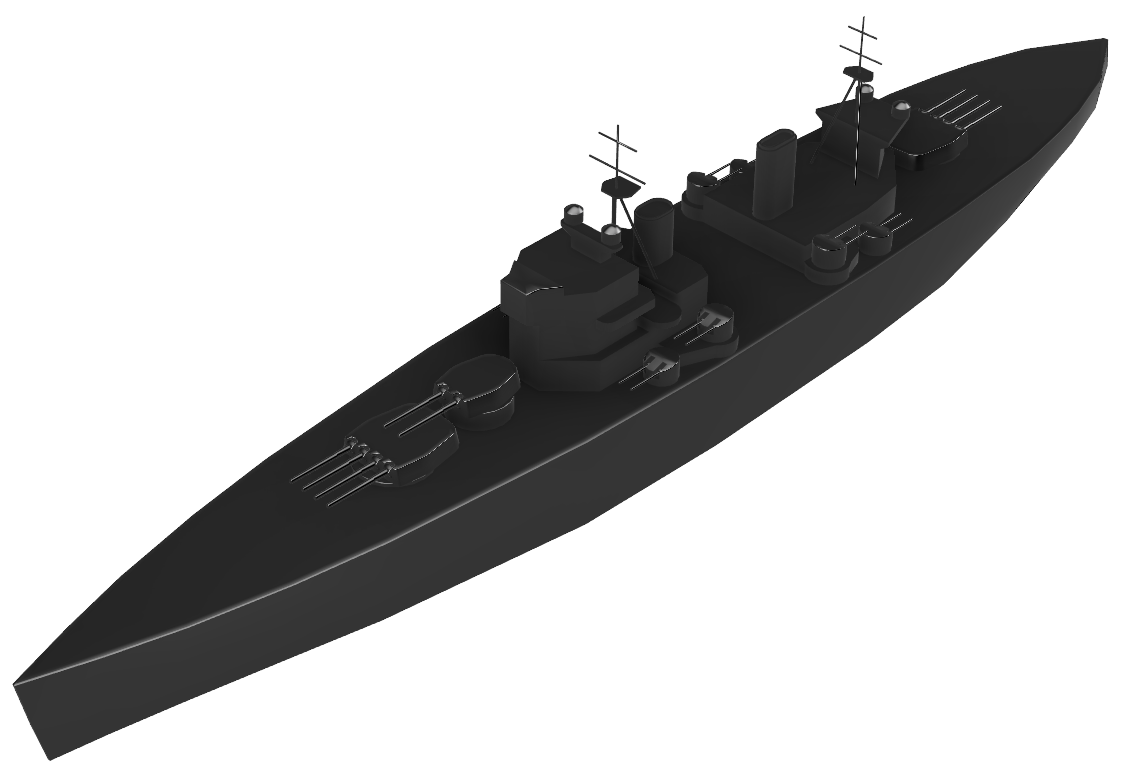
\includegraphics[width=0.25\textwidth]{background/ship_000090}\label{subfig:ship_000090}}
    \subfloat[Desired: $\langle90, 0, 0\rangle$]{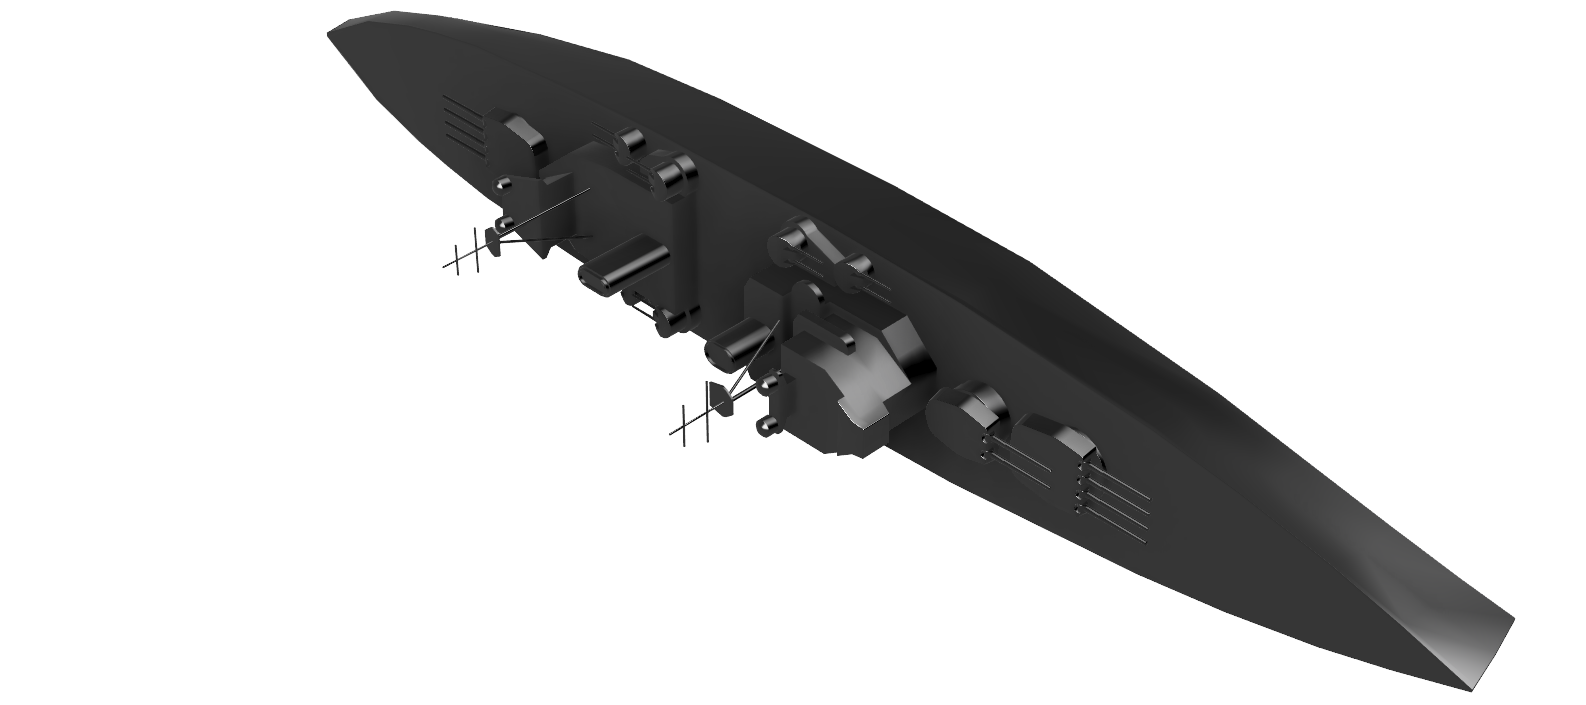
\includegraphics[width=0.25\textwidth]{background/ship_900000}\label{subfig:ship_900000}}
    \caption[Gimbal lock demonstration]{Demonstration of gimbal lock on a rotating 3D body.
    Despite only pitching and rolling the body, the end result of the transformation is an effective yaw.
    This is because the first pitch aligns the roll and yaw axes, effectively making them the same.
    In the given rotation order, any roll rotation would be equivalent to a yaw rotation when the object is pitched 90$^{\circ}$.
    \textit{3D model courtesy of "printable models" from Free3D.com.}}
\end{figure}

\subsection{Quaternions} \label{ssec:quaternions}
In the 19th century, an Irish mathematician was contemplating the problem of Euler angles and analyzing three dimensional geometry.
William Hamilton considered the problem from within the complex or imaginary space and found that a three dimensional vector could not be expressed with a complex triplet.
Instead, Hamilton discovered that the problem could be solved with a complex quadruplet, called a quaternion [CITE - On Quaternions], which could be used as a more mathematically pure tool to understand three dimensional geometry.
For more detailed notes, see Appendix \ref{chap:quaternions}.

A quaternion exists in four dimensional Hamiltonian space and has three complex and one real component in its vector. 
Like a rotation matrix, it describes the rotation from one reference frame to another about some axis, $\vec{r}$, as shown in Figure \ref{fig:frame_rotation}.
But, the quaternion is not susceptible to gimbal lock as when two of its axes align, it still retains three degrees of freedom.
Additionally, it is not limited to the range of 0 to 360 (or -180 to 180) like Euler angles and therefore has no discontinuities.
We can express the quaternion from frame $A$ to frame $B$ as:

\begin{equation*}
    {}^A_B \vec{q} = \left[
        \begin{matrix}
            q_1 & q_2 & q_3 & q_4
        \end{matrix}
    \right] = 
    \left[
        \begin{matrix}
            w & x & y & z
        \end{matrix}
    \right] = 
    w + x\hat{i} + y\hat{j} + z\hat{k}
\end{equation*}

Since the quaternion is just a vector, this drastically simplifies any rotation calculations and improves computational performance.
In order to rotate a vector using a quaternion, we need to set the quaternion to be a unit quaternion by:

\begin{equation*}
    q = \frac{q}{|q|}
\end{equation*}

Then, we can calculate the inverse quaternion, ${q}^{-1}$ (or conjugate $q^*=q^{-1}, \text{ if } |q|=1)$, using:

\begin{equation*}
    q^{-1} = \frac{q_0 - q_1\hat{i} - q_2\hat{j} - q_3\hat{k}}{|q|^2}
\end{equation*}

Then, we can rotate the vector using the equation:

\begin{equation*}
    {}^A \vec{v}_B = {}^A_Bq \vec{v}_A {}^A_Bq^{-1}
\end{equation*}

In an inertial measurement unit or attitude and heading reference system, we will need to rotate freely between readings taken in the body's local frame to that in the global frame, such as determining linear acceleration.
Using the quaternion method above we can also relate body measurements to the global frame, which can be useful for other analyses.

\section{Sensing} \label{sec:sensing}
Now that we have a basic understanding of some of the mathematical relationships present in inertial tracking, we need to start sensing our environment.
So, how can we compute the position, velocity, acceleration, and attitude of a body in space?
In order to answer this question, we must first examine the different sensors that are available.

\subsection{Magnetometer} \label{ssec:magnetometer}
Magnetometers use magnetoresistive elements that change their effective resistance in the presence of a magnetic field [CITE - Robotics, Vision and Control].
Atoms within a magnetoresistive element change their orientations with the magnetic field.
The new orientation can hinder or aid the path of free electrons moving through the element, thus changing the resistance.
By measuring this value and correlating it to a measurement scale, the local magnetic field can be determined.

\begin{figure}[h!]
    \caption[Magnetometer block diagram]{Basic block diagram of a single-axis magnetometer where electrons are flowing through the magnetoresistive material. The left diagram shows the condition when the magnetic field is aligned (minimal resistance); the right shows the non-aligned magnetic field condition which increases the resistance the electrons face passing through the material.}
    \label{fig:magnetometer}
    \centering
    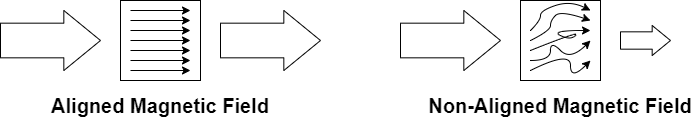
\includegraphics[width=4.5in]{background/magnetometer.png}
\end{figure}

\subsection{Gyroscope} \label{ssec:gyroscope}
A gyroscope is an inertial sensor that measures the angular velocity of a rotating body.
MEMS-based gyroscopes measure this value by applying the Coriolis effect on a microscopic mass [CITE - Robotics, Vision and Control].
As shown in Figure \ref{fig:gyroscopes}, an oscillation is induced on the x-axis using a driving circuit.
While oscillating, if an angular velocity ($\omega$) is imparted on the z-axis, the suspended mass will experience a force in the y-axis that is proportional to $\omega$ (Appendix [INSERT APPENDIX NUMBER]).
Since the mass is suspended on springs, Newton's Second Law can be applied again to directly correlate the force experienced to a displacement and therefore a change in resistance or capacitance.

\begin{figure}[h!]
    \caption[Gyroscope block diagram]{Basic block diagram of a three-axis gyroscope where the masses are suspended from springs. The left diagram shows a single mass configuration; the right shows a tuning fork configuration which is twice as sensitive as the singular mass.}
    \label{fig:gyroscopes}
    \centering
    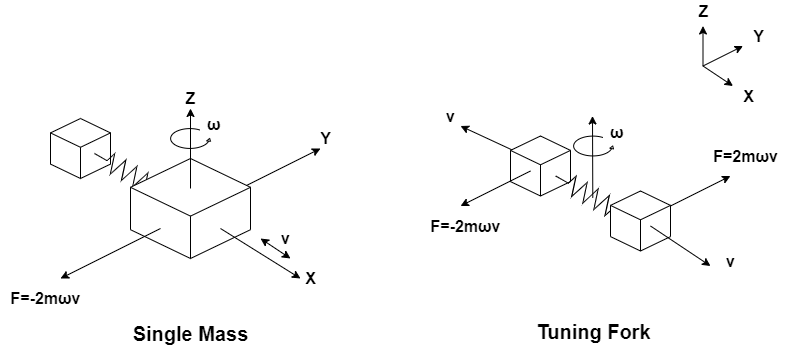
\includegraphics[width=4.5in]{background/gyroscopes.png}
\end{figure}

\subsection{Accelerometer} \label{ssec:accelerometer}
Accelerometers measure a change in velocity over time (acceleration).
An accelerometer is comprised of a mass suspended in an axis of motion by springs of a known K-constant [CITE - Robotics, Vision and Control].
From Newton's Second Law, as applied to a spring-mass system, $\frac{-K}{m}x=a$, we can directly correlate the displacement of the mass to the magnitude of the acceleration along the measurement axis.
Typically, this scale is electrically resistive or capacitative and creates an analog change in a driving (exciting) voltage which can be measured in a circuit using a Wheatstone Bridge and microcontroller.
A basic representation of a three-axis accelerometer is shown in Figure \ref{fig:accelerometers}.

\begin{figure}[h!]
    \caption[Accelerometer block diagram]{Basic block diagram of a three-axis accelerometer where the masses are suspended from springs.}
    \label{fig:accelerometers}
    \centering
    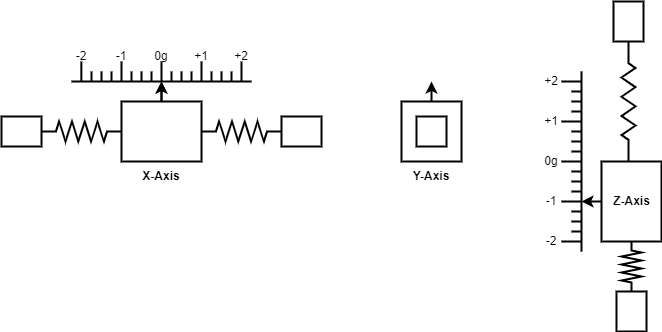
\includegraphics[width=4.5in]{background/accelerometers.png}
\end{figure}

\subsection{MARG Arrays and Inertial Measurement Units} \label{ssec:marg_imu}
Now, with the basics of each sensor in mind, we can combine them into a single package, called a Magnetic, Angular Rate, and Gravity (MARG) array.
Each of the above diagrams represent a single sensing axis, or Degree of Freedom (DOF).
In order for a MARG array to be useful in a 3D environment, it needs to have three sensing axes orthogonal to each other.
Each DOF will measure the X-, Y-, and Z-axis, respectively with the positive sensing direction according to the right hand rule.
By combining multiple tri-axial arrays, we can define different types of Inertial Measurement Units (IMUs), as shown in Table \ref{tab:imu_dofs}.
Typically, the more sensing axes, the more accurate the array will be (depending on the performance of the sensor fusion algorithm).
Note that a MARG array is an IMU with an integrated tri-axial magnetometer .

\begin{table}[h]
    \caption{Common definitions for IMUs of varying degrees of freedom.}
    \label{tab:imu_dofs}
    \centering
    \begin{tabular}{| c | c | c | c | c |}
        \hline
        DOFs & Accelerometer & Gyroscope & Magnetometer & Barometer \\
        \hline
        3-DOF & 3-axis\footnote[2]{can be either or} & 3-axis\footnote[2] & --- & --- \\
        6-DOF & 3-axis & 3-axis & --- & --- \\
        9-DOF & 3-axis & 3-axis & 3-axis & --- \\
        10-DOF & 3-axis & 3-axis & 3-axis & 1-axis \\
        \hline
    \end{tabular}
\end{table}

\begin{figure}
    \begin{fitbox}[frametitle=Aside: MEMS Technology]
        During the Apollo program, the ST124-M inertial measurement unit was developed that fed the Saturn V rocket's inertial characteristics to the main flight computer [CITE - ST124-M description].
        The IMU consisted of a tri-axial gyroscope array, redundant tri-axial accelerometer arrays, pendulums, and other sensors.
        While it was a technological marvel at the time, it was the size of a basketball and weighed about 45-65 kilograms.
        Modern cellphones with the same capability are orders of magnitude smaller, lighter, and cheaper; so, what happened?

        \begin{center}
            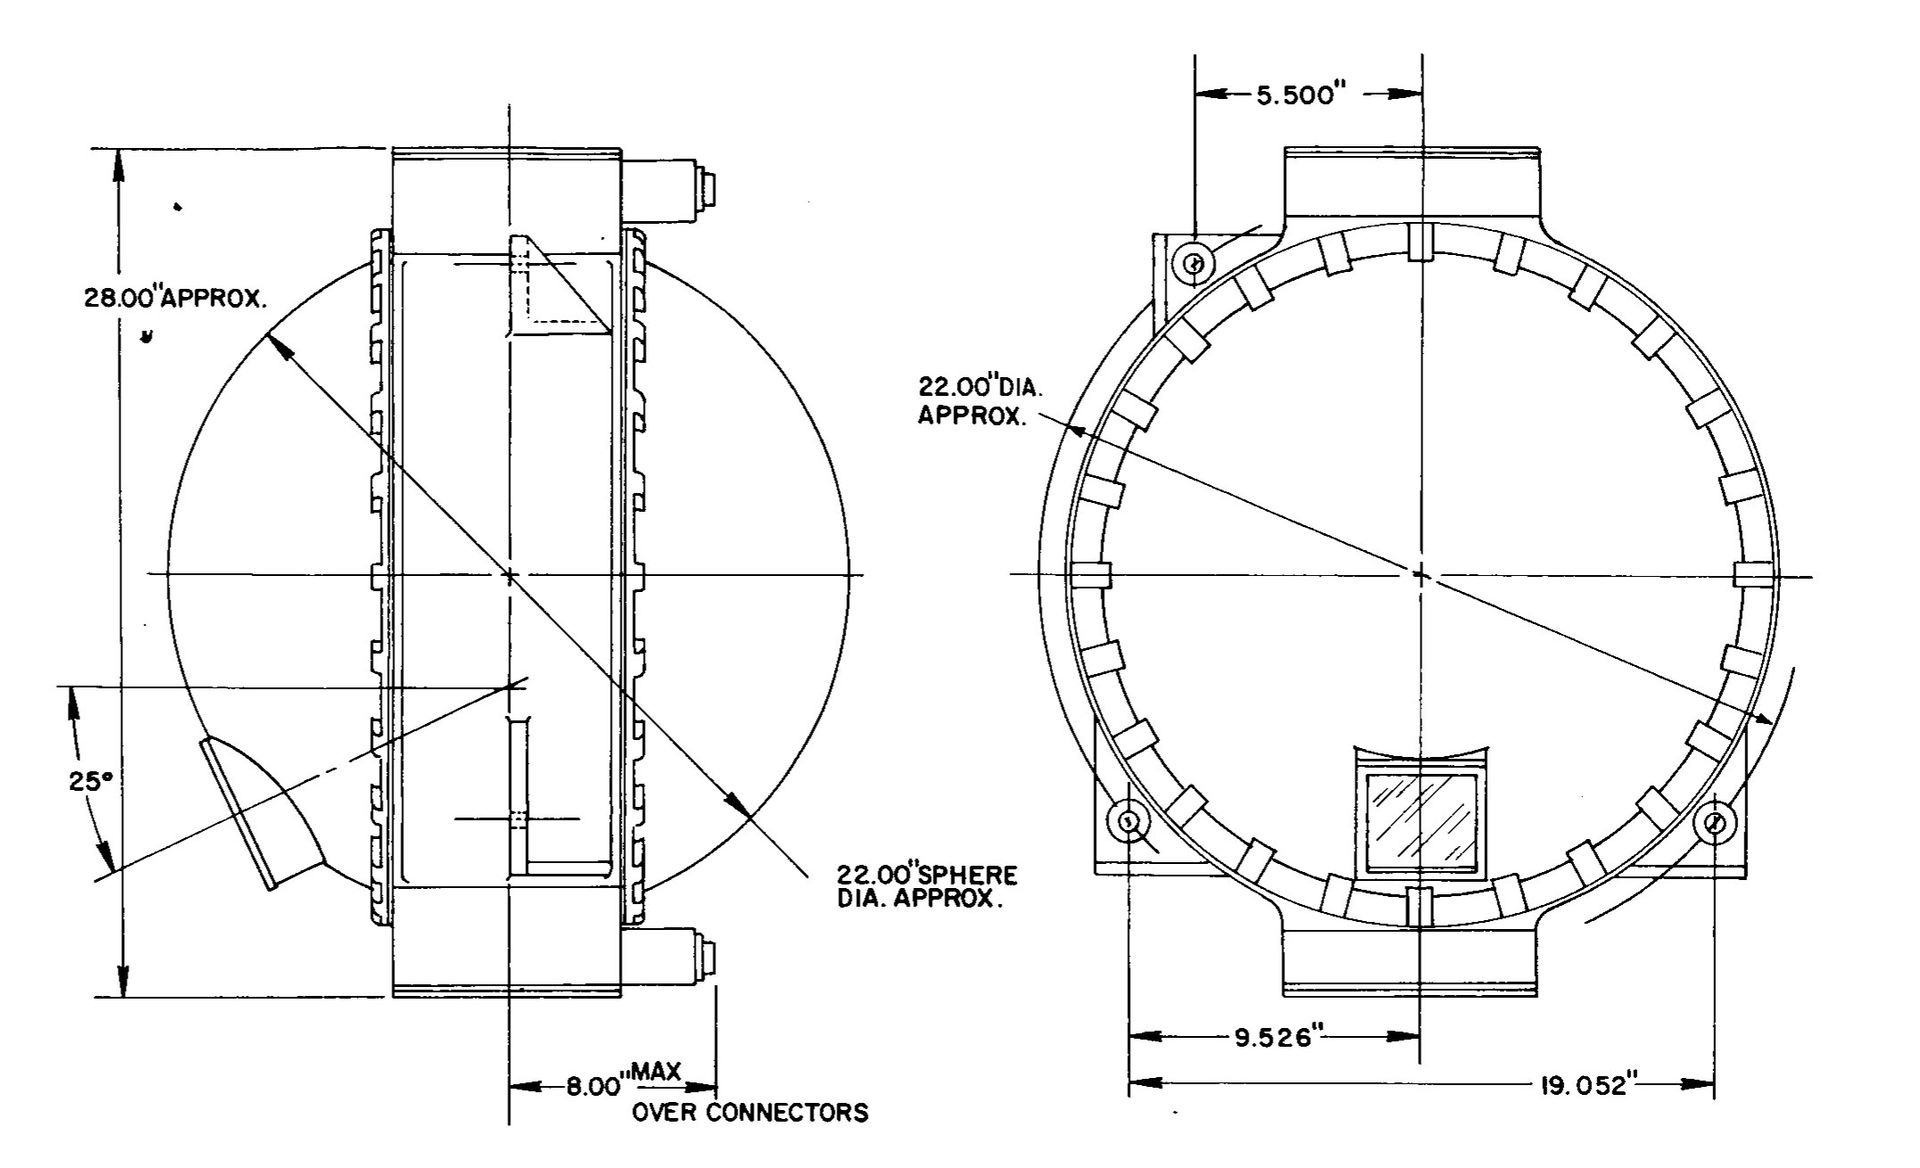
\includegraphics[height=3in]{images/background/Apollo_IMU_exhibit.jpg}
            % \caption[Test]{ST124-M inertial measurement unit courtesy of NASA \url{https://en.wikipedia.org/wiki/ST-124-M3_inertial_platform#/media/File:ST124-M_drawing.jpg}}
            \caption[ST124-M Outline]{ST124-M inertial measurement unit courtesy of NASA via Wikimedia Commons [CITE - Wikimedia]}
        \end{center}

        Modern manufacturing methods have enabled a new technology called Microelectromechanical Systems, or MEMS.
        MEMS are microscopic devices that perform an electromechanical function such as sensing acceleration, rotation rate, or magnetic fields [CITE - What is MEMS].
        They are the most common technology in modern sensor development and revolutionized the technology space by shrinking components down to the micro- and nanometer scales.
        Due to the advent of MEMS technology, devices such as accelerometers, magnetometers, gyroscopes, barometers, hygrometers, etc. have been shrunk down from large mechanical masterpieces to mass-producible products that fit within a few square millimeters of epoxy.
        This dramatically cheapened these devices and has allowed more products to integrate smart sensors into their designs.
    \end{fitbox}
\end{figure}

According to VectorNav [CITE], a producer of industrial-grade IMUS, the cheapest, least precise, and least accurate IMUs are considered "consumer-grade".
Every day smartphones, cheap commercial breakout boards, and even shipping crates have these devices on-board.
Consumer-grade IMUs can be bought for cents, dollars, or tens of dollars per unit in bulk and are ideal for mass production spaces where quantity is king over quality.
A step up from these sensors are "industrial-grade" IMUs. 
These are tens to hundreds of dollars per unit but are an order of magnitude more accurate and precise than their consumer counter parts.
This makes them desirable for the automotive and industrial sectors as they can assist in automation, control, and monitoring of expensive unmanned systems.
The "tactical-grade" sensors are even more robust and accurate than the previous tiers and have an appropriate military-industrial complex price tag to match. 
These devices will typically be used in applications where war fighters need precise guidance for munitions, or need to navigate their way through hazardous and GNSS-denied terrain.
Finally, the last major tier is the "navigation-grade" sensors. 
These sensors are extremely precise, extremely accurate, and cost more than some middle-class families will make in a year.
Primarily, these will be used in survey missions or on underwater vehicles where absolute precision and knowledge of their location is necessary.

\subsection{Global Positioning System} \label{ssec:gps}
The Global Position System, or GPS, is a constellation of high-altitude satellites that service most of the globe [CITE].
First developed by the US military for large scale maneuvers on the battlefield, GPS is a ubiquitous technology that is available in almost every device from smartphones to cars.
Each GPS satellite in orbit transmits the current time measured by their internal atomic clocks.
A GPS receiver on the ground can synchronize its own internal clock to the GPS time and wait for a satellite's transmission.
When the satellite time is received, the device can determine the difference between its clock and the satellite's report called the Time of Flight.
Since the Time of Flight can be assumed to be the constant speed of light, the GPS receiver can determine its distance to a satellite in a known orbit.
Repeat for at least three satellites, and a GPS receiver can triangulate its position to a reasonable circle of error of about 3-meters.

\begin{figure}[h!]
    \caption[GPS diagram]{Basic representation of how GPS communicates with a device to calculate its position on Earth.
    GPS satellites in orbit broadcast a time and using trigonometry and algebra, a device can calculate the distance to various satellites and triangulate its position.}
    \label{fig:gps}
    \centering
    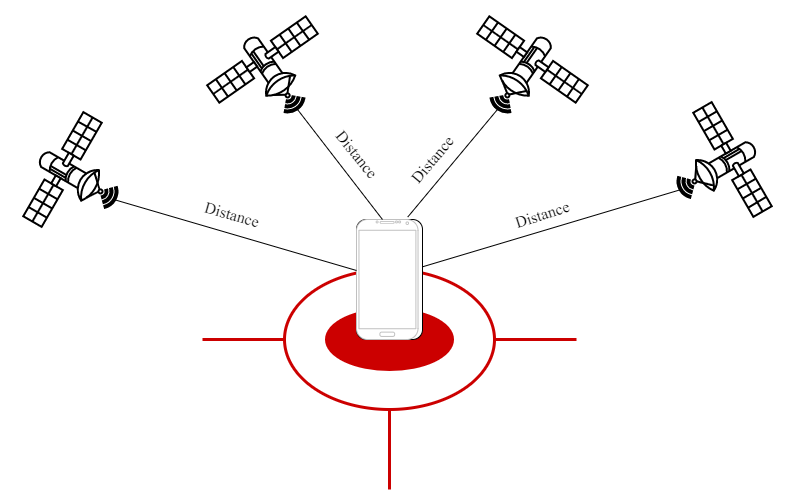
\includegraphics[width=4.5in]{background/gps.png}
\end{figure}

\section{Sensor Fusion} \label{sec:sensor_fusion}
While having each individual sensor will give some data, they offer an incomplete picture of a body's orientation and movement through space.
An accelerometer can detect acceleration and determine pitch and roll using basic vector math, but it cannot determine yaw or heading.
Data from a gyroscope can be integrated over time to determine the sensor's attitude, but this method will drift over time and accumulate errors, it also cannot detect movement.
Magnetometers in a weak magnetic field, like Earth's, are not accurate enough to determine roll and pitch, but can easily provide heading.
Finally, GPS readings will provide position and velocity vectors, but typically update slowly and have a large circle of error and cannot determine attitude.
In order to make these sensors more effective for an inertial sensing application, we need to fuse the data feeds into a unified output that emphasizes the strength of each sensor, while mitigating their limitations.

\subsection{Attitude and Heading Reference System} \label{ssec:ahrs}
An Attitude and Heading Reference System (AHRS) is an IMU equipped with an accelerometer, gyroscope, and/or a magnetometer in all three axes.
The data streams from the sensors can be fused together with external information like GPS data and mathematical models to estimate a body's inertial orientation in three dimensional space.
The block diagram for this operation is shown in Figure \ref{fig:ahrs_design}.
Many algorithms exist to do this sensor fusion such as the Kalman filter [CITE - Kalman], the Mahony filter [CITE], the Madgwick filter [CITE], and the Fast Complimentary Filter [CITE].

\begin{figure}[h!]
    \caption[AHRS block diagram]{Basic block diagram of an AHRS. 
    The acceleration, rotation rates, and magnetic field readings are fused together in the IMU. 
    The AHRS can then apply a bias from the GPS course and corrections from a mathematical model of the system.}
    \label{fig:ahrs_design}
    \centering
    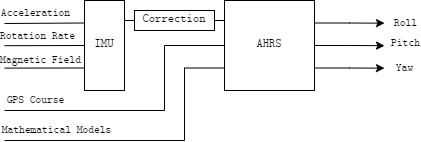
\includegraphics[height=1.3in]{background/ahrs.png}
\end{figure}

\subsection{Fast Complimentary Filter} \label{ssec:complimentary_filter}

\subsection{Kalman Filter} \label{ssec:kalman_filter}
The Kalman Filter is a recursive algorithm introduced in the 1960's as a method to track, estimate, and predict the state of a system and corresponding uncertainties [CITE].
This filter integrates a dynamic (linear) model of the system, control inputs, measurements, and biases/uncertainties into a single algorithm.
This effectively fuses together system inputs and responses and extrapolates what the system is currently doing and expected to do.
One key advantage of this algorithm is that it only requires the guess of the previous state to estimate the current state. 
This massively decreases the memory and processing costs as the history of inputs, measurements, and uncertainties does not need to be remembered or analyzed.
However, it does have some limitations when the sensor data is noisy or the control inputs cannot be linearly mapped to the system state.
Random errors in the sensor data may cause the filter to behave unpredictably and non-linearity prevents proper fusion entirely.

The algorithm works by taking uncertainties from sensor measurements and using those to determine the Kalman Gain factor, $K_n$.
This gain is the magnitude of the uncertainties from the previous estimate and measurement sources.

\begin{equation} \label{eq:kalman_gain}
    \begin{aligned}
        K_n &= \frac{\text{Estimate Uncertainty}}{\text{Estimate Uncertainty + Measurement Uncertainty}} \\
            &= \frac{p_{n,n-1}}{p_{n,n-1} + r_n}
    \end{aligned}
\end{equation}

The gain is then applied to a state update equation where the current estimate of the sensor values is determined. S

\begin{equation} \label{eq:kalman_state_update_eq}
    \begin{aligned}
        \hat{x}_{n,n} &= \hat{x}_{n,n-1} + K_n(z_n - \hat{x}_{n,n-1}) \\
                      &= (1-K_n)\hat{x}_{n,n-1} + K_n z_n \\
    \end{aligned}
\end{equation}

On the first run of the algorithm, an initial state guess and uncertainty are introduced as a starting point for the state prediction equation.
This equation is the mathematical model of the system and, for example, can be the Newtonian equations of motion for a moving body.
This creates a prediction for the next state.
The algorithm can then output the current state, predicted next state, and associated uncertainties with reasonably high accuracy - assuming the filter is tuned.
Tuning the filter can be done by better quantifying the measurement errors and by tuning hyperparameter called "process noise variables".
These variables control how much the algorithm depends on the measurement or the previous estimate to make the current and future estimates.

\begin{figure}[h!]
    \caption[Kalman filter block diagram]{Basic block diagram of a Kalman filter.}
    \label{fig:kalman_filter}
    \centering
    \includegraphics[width=6in]{background/KalmanFilter.png}
\end{figure}

\subsection{Mahony Filter} \label{ssec:mahony_filter}
A popular AHRS sensor fusion algorithm is the Mahony filter [CITE].
This algorithm estimates the rotation rate, $\pmb{\omega}'$ of the body given the instantaneous rotation rate, $\pmb{\omega}$ and acceleration vector, \pmb{a}.
The error, $e$, is calculated as the cross-product between the current acceleration vector and the expected gravitational acceleration vector from the previous estimate.
The filter uses a Proportional-Integral (PI) controller to determine the filter error from the previous estimate and apply a bias, $\delta\omega$ to the current estimate.
By integrating $\omega'$, the estimated attitude can be determined.
The equation for a basic Mahony figure is given below:

\begin{gather}
    \label{eq:mahony_filter}
    \pmb{\omega}' = \pmb{\omega} + \left(K_p + K_i\frac{1}{s}\right) \pmb{a} \times \pmb{d} \\
    \begin{aligned}
        \text{where } & \pmb{\omega} \text{ is the instantaneous rotation rate vector} \\
        & K_p \text{ is the proportional controller constant} \\
        & K_i \text{ is the integral controller constant} \\
        & \pmb{a} \text{ is the instantaneous acceleration vector} \\
        & \pmb{d} \text{ is the estimated gravity vector from the previous estimate} \\
    \end{aligned} \notag
\end{gather}

This filter is used to fuse 6DOF IMU data, but is limited as the yaw orientation cannot be known or calculated; it also does not account for gyroscopic drift which decreases its accuracy over time.
Additionally, this filter primarily works in the Eulerian coordinate system, which causes singularities and discontinuities due to gimbal lock.

\subsection{Madgwick Filter} \label{ssec:madgewick_filter}

\subsection{Inertial Calibration}

In order to calibrate an IMU, we need to create a model of the data. For the accelerometer and gyroscope, we can create an inertial model defined as:

\begin{gather}
    \vec{i}_c=MS(\vec{i}_u-\vec{b}) \\
    \begin{aligned}
        \text{where } & \vec{i}_C \text{ is the calibrated inertial measurements,} \\ 
        & M \text{ is the misalignment matrix,} \\
        & S \text{ is the sensitivity identity matrix,} \\
        & \vec{i}_u \text{ is the uncalibrated inertial measurements, and} \\
        & \vec{b} \text{ is the bias or offset vector}
    \end{aligned} \notag
\end{gather}

The three calibration values, $M$, $S$, $b$, represent a set of correction factors that make the measured values more accurate. The inertial measurement is generalized here to represent either accelerometer or gyroscope data. Each sensor will have its own set of the calibration values.

\paragraph*{Bias Vector} The bias, or offset, vector is the average of the inertial readings while the sensor is in a stable, known orientation. For example, when the gyroscope is at rest, we would expect the measurement output to be $[0,0,0] \text{ [deg/sec]}$. However, we may measure an average of $[0.89, -0.66, 0.31] \text{ [deg/sec]}$ instead. By subtracting this bias vector from the measurements, we eliminate any unintentional offset from our readings. The bias can be calculated using the equation below:

\begin{gather}
    \vec{b}_g = \frac{1}{N} \sum_{i=0}^N{\vec{g}_n} \\
    \begin{aligned}
        \text{where } & \vec{b}_g \text{ is the bias vector,} \\
        & N \text{ is the number of collected samples to average, and} \\
        & \vec{g}_n \text{ is the n-th uncalibrated gyroscope measurement vector in the dataset}
    \end{aligned} \notag
\end{gather}

For accelerometers, the bias is calculated differently. Each measurement axis must be exposed to ±1g of acceleration by placing the instrument vertical on each of the measurement axes in both the positive and negative directions. The bias for each axis can then be determined by taking the average value as shown below:

\begin{gather}
    \vec{b}_a = \frac{1}{2} \left[ \frac{1}{N}\sum_{n=0}^N{\vec{a}_{n,+g}} + \frac{1}{M}\sum_{m=0}^M{\vec{a}_{m_-g}} \right] \\\
    \begin{aligned}
        \text{where } & b_a \text{ is the bias vector,} \\
        & N \text{ is the number of samples taken in the +1g orientation,} \\
        & a_{+g} \text{ is the average axis measurement when exposed to +1g, and}\\
        & M \text{ is the number of samples taken in the -1g orientation,} \\
        & a_{-g} \text{ is the average axis measurement when exposed to -1g}
    \end{aligned} \notag
\end{gather}

\paragraph*{Sensitivity Matrix} The sensitivity matrix is a diagonal matrix that accounts for minor errors with variations in process and material. 
This can make each uniaxial sensor in a triaxial array sense the environment slightly differently. 
While bias covers this area when at rest or in specific orientations, the sensitivity error will change depending on the motion and orientation. 
To account for this, we need to expose each sensor to a known reference stimulus and calculate a sensitivity value based on the average magnitude of the measurement vector during that time. 
For a gyroscope, this value can be an arbitrary, but constant, rotation rate, $\omega$. 
For an accelerometer, this value will be ±1g. The equations for each gyroscope and accelerometer axis are provided below:

\begin{gather}
    s_{g, \omega} = \frac{\lVert g_{+\omega}\rVert + \lVert g_{-\omega}\rVert}{2\omega} \\
    \begin{aligned}
        \text{where } & s_{g,\omega} \text{ is the sensitivity value for each gyroscope axis when exposed to } \omega , \\
        & g_{+\omega } \text{ is the average gyroscope axis reading whe exposed to +} \omega ,\\
        & g_{-\omega } \text{ is the average gyroscope axis reading whe exposed to -} \omega , \text{ and} \\
        & \omega \text{ is the reference rotation rate}
    \end{aligned} \notag
\end{gather}

\begin{gather}
    s_{a, g} = \frac{\lVert a_{+g} \rVert + \lVert a_{-g} \rVert}{2} \\
    \begin{aligned}
        \text{where } & s_{a,g} \text{ is the sensitivity value for each axis when exposed to 1g,} \\
        & a_{+g} \text{ is the average axis measurement when exposed to +1g, and} \\
        & a_{-g} \text{ is the average axis measurement when exposed to -1g}
    \end{aligned} \notag
\end{gather}

After calculating these values for each axis, we can form the sensitivity matrix for the gyroscope and accelerometer like so:

\begin{equation*}
    S_g = 
    \begin{bmatrix}
        s_{g,x} & 0 & 0 \\
        0 & s_{g,y} & 0 \\
        0 & 0 & s_{g,z}
    \end{bmatrix} 
\end{equation*}
\begin{equation*}
    S_a =
    \begin{bmatrix}
        s_{a,x} & 0 & 0 \\
        0 & s_{a,y} & 0 \\
        0 & 0 & s_{a,z}
    \end{bmatrix}
\end{equation*}

While this calibration value accounts for some of the intrinsic sensor error, it does not account for axes misalignment or non-orthogonality within the sensor. To accomplish this, we must incorporate the misalignment matrix.

\paragraph*{Misalignment Matrix}

The misalignment matrix is the final, but most complex, calibration value that we can calculate for the inertial sensors. It reduces error from multiple sources such as non-orthogonality between the measurement axes, the misalignment from the measurement axes to the actual sensor packaging, and misalignment from the package onto the application board. In order to calculate the misalignment matrix, we must consider it as the solution to a non-linear problem. First, we must define an objective function for the solution space. Since the goal of the misalignment matrix is to reduce error, then we can define the objective function as the Root Mean Square Error (RMSE) of the measurement vector, the misalignment vector, and the reference vector:

\begin{gather}
    RMSE = \sqrt{\frac{1}{N}\sum_{n=0}^N{\|{\vec{i}_{n,u} \cdot M^* -\vec{i}_{n,ref}\|}^2}} \\
    \begin{aligned}
        \text{where } & N \text{ is the number of samples in the dataset,} \\
        & \vec{i}_{n,u} \text{ is the n-th uncalibrated measurement vector with the bias removed,} \\
        & M^* \text{ is the guessed 3-by-3 matrix that corrects $i_{n,u}$ to be near $i_{ref}$, and } \\
        & \vec{i}_{ref} \text{ is the expected reference stimulus vector for the measurement}
    \end{aligned} \notag
\end{gather}

Then, given a dataset of measurement vectors and their expected reference vectors, we can use a non-liner solver to determine the value of $M^*$. This can be done using toolboxes \footnote[4]{Like the \href{https://docs.scipy.org/doc/scipy/reference/generated/scipy.optimize.minimize.html}{\lstinline{scipy.optimize.minimize} toolbox}}. 
Assuming the sensitivity was not removed from the measurement signal, the $M^*$ matrix happens to include it as its diagonal. 
By extracting the diagonal and normalizing the original matrix, we are left with the sensitivity and misalignment matrix calibration values.

\begin{equation*}
    S = \text{diag}(M^*) \\
    M=M^* \cdot S^{-1}
\end{equation*}

We can now apply the misalignment matrix, sensitivity matrix, and bias vector to the sensor readings according to the model above. This should yield outputs that are close to the real values, which is examined in the next section.

\subsection{Magnetic Calibration}
The magnetometer in a MARG array needs a different sensor model than the inertial sensors because the ambient magnetic field introduces different errors. 
There are two types: soft iron, $W$, and hard iron, $\vec{v}$. 
A hard iron distortion is introduced by magnetic materials placed near the sensor. 
This can occur when the sensor is placed in a casing with magnetic fasteners or a speaker, as shown in Tuupola [CITE - Tuupola]. 
Soft iron distortion is typically less severe than hard iron distortion and is caused by materials near the sensor that distort the local magnetic field. 
The soft iron distortion can also account for misalignment and sensitivity errors. 
The sensor model for a calibrated magnetometer is given below:

\begin{gather}
    \vec{m}_c=W^{-1}(\vec{m}_u-\vec{v}) \\
    \begin{aligned}
        \text{where } &\vec{m}_c \text{ is the calibrated magnetometer vector,} \\
        &W^{-1} \text{ is the inverse soft iron matrix,}\\
        &\vec{m}_u \text{ is the uncalibrated magnetometer vector,} \\
        &\vec{v} \text{ is the hard iron bias vector}
    \end{aligned} \notag
\end{gather}

With a calibrated sensor in an ideal environment, we would expect a sphere centered on the origin with a radius equal to the magnitude of the local magnetic field. 
Due to the hard and soft iron distortions, this will rarely be the case. 
Hard iron distortion can be removed from the signal by determining the average of the minimum and maximum values of each axis, as shown below:

\begin{equation*}
    \vec{v}=\frac{1}{2}
    \begin{bmatrix}
        \max(v_x)+\min(v_x) \\
        \max(v_y)+\min(v_y) \\
        \max(v_z)+\min(v_z)
    \end{bmatrix}
\end{equation*}

Once the hard iron distortion is removed from the signal, we should see the readings more closely adhere to the correct spherical shape. 
Then, we can apply Li’s ellipsoid fitting algorithm[CITE - Li] to characterize the fit of the optimal ellipsoid for the data, expressed as the symmetrical matrix, $A$. 
Ozyagcilar [CITE - AN4246] delves into the math and builds a relationship between the ellipsoid fit and the soft iron matrix, summarized by:

\begin{equation*}
    W^{-1}=A^{1/2}
\end{equation*}

With these calibration parameters calculated, they can be used in a sensor fusion algorithm to increase the accuracy of the magnetometer. 
However, these parameters must be recalibrated whenever the sensor enters a new magnetic environment since either the hard or soft iron distortion could be different than previously calculated.

[TODO: INSERT FIGURES OF MAGNETIC CALIBRATION AND DISTORTION]
%%--------------------Chapter 3------------------------
\chapter{Thetis Design} \label{chap:thetis_design}

\section{Stakeholders} \label{sec:stakeholders}
As with any project, stakeholders are a crucial part of the design process.
Stakeholders drive certain requirements that the device must achieve in order to be accepted for operation.
On an individual level, the committee overseeing this thesis are the major stakeholders as they have a vested interest in the success or failure of the project.
However, there are some organizational-level stakeholders that have also expressed interest in the project and provided some feedback for their requirements.
A summary of the stakeholders is provided in Table \ref{tab:stakeholders}.

\begin{table}
	\caption{A summary of stakeholders of the Thetis device}
	\label{tab:stakeholders}
	\centering
	\begin{tabular}{|p{0.3\linewidth} | p{0.6\linewidth}|}
		\hline
		\rowcolor[gray]{0.8}
		\multicolumn{1}{|c|}{\textbf{Stakeholder}} & \multicolumn{1}{|c|}{\textbf{Description}} \\
		\hline
		Committee members & Individual professors who have expressed interest in the project and have agreed to assist in its development. Specifically, Dr. Wood and Dr. Weaver would like to deploy Thetis on university projects; Dr. Gutierrez has provided many requirements on the performance of the instrumentation; and Dr. Silaghi is interested in its application to autonomous navigation. \\
		\hline
		Florida Institute of \newline Technology & The university has several classes and projects where the Thetis design could be useful. The Instrumentation Design and Analysis class used Thetis as a demonstrator for designing PCBs and field experiments. Thetis was also designed with Surf Engineering Analysis in mind for students to have a new open source sensor to experiment with. \\
		\hline
		Maritime Tactical \newline Systems (MARTAC) & This corporation has expressed interest in using Thetis for research and characterizing the performance of their high speed catamarans in open-water testing \\
		\hline
		NSWC Carderock - \newline Combatant Craft Division (CCD) & This three-letter agency of the government has expressed interest in using Thetis as a testing and evaluation tool for small unmanned crafts \\
		\hline
	\end{tabular}
\end{table}

\subsection{Hands-On Users} \label{ssec:hands_on_users}

\section{Design Rationale} \label{sec:design_rationale}
Thetis is envisioned as an open-source all-in-one data logging solution for use in research projects.
The device incorporates multiple sensors, GPS tracking, and a WiFi-capable microcontroller in order to enable as many features as can be envisioned by the end users.
One of the driving considerations was the small footprint.
Thetis Revision F is designed to fit into one of the smallest IP67-rated enclosures available on the market [LINK].  
This tiny form factor allows it to be inconspicuously mounted to any floating body like surfboards, scale models, or wave buoys without upsetting their inertial characteristics or impeding nominal operation.

Further discussions with stakeholders later in the design process envisioned a new iteration, Revision G, that had a larger footprint, but added more capabilities like CANbus integration and several connection ports for different communication protocols.
This revision is meant for deployment on vessels that have a NMEA2000 communications bus.
This bus allows the device to be powered from the boat's power supply and communicate data to a central controller.
These features are extremely important for the final application where Thetis is meant to feed data into a navigation algorithm for the safe passage of unmanned vessels.

\subsection{Problem Description} \label{ssec:problem_desc}
Tracking the inertial movements of small floating bodies in-situ is difficult for small-scale or student-led experiments.
The price of the measurement instruments and the data acquisition computers (DAQs) offers a high bar for entry for these projects.
Also, the size of these instruments and DAQs can negatively impact the performance or operation of small floating bodies so they cannot be effectively used.
This forces classrooms and organizations to either neglect collecting inertial data or using bulky, unreliable prototype setups using off-the-shelf components

\subsection{Mission Statement} \label{ssec:mission_statement}
Thetis aims to democratize the inertial measurement and tracking space for small scale experiments by implementing an open-source, feature-rich, all-in-one solution to monitoring the movements of floating bodies.

\subsection{Stakeholder Requirements} \label{ssec:stakeholder_reqs}
Interviews with the stakeholders occurred over several months and informed a set of requirements that they determined were necessary for the project's success.


\subsection{Feasibility and Risk Identification} \label{ssec:feasibility_risk}
The following tables provide the supporting documentation to the requirement feasibility assessment for technical, cost and schedule, organizational, and political and operational. The conclusion is that all requirements have been proven feasible with current technology.

\begin{landscape}
% ==================================
% === STAKEHOLDER REQUIREMENT XX ===
% ==================================

% \paragraph{S.R. XX} - The requirement

% {\fontsize{10pt}{11pt}\selectfont
% \begin{longtable}{| p{0.12\linewidth} | p{0.16\linewidth} |  p{0.20\linewidth} | p{0.08\linewidth} | p{0.20\linewidth} | p{0.08\linewidth} |}
%     \hline \endlastfoot
	
%     \hline
%     \rowcolor[gray]{0.8}
%     \multicolumn{6}{|c|}{ } \\
%     \hline
%     \textbf{Stakeholder:} & \multicolumn{5}{|l|}{Wilford Erasmus, POC of the three-letter agency} \\
%     \hline
%     \textbf{Rationale:} & \multicolumn{5}{|L{0.8\linewidth}|}{s} \\
%     \hline
%     \textbf{Fit Criterion:} & \multicolumn{5}{|L{0.8\linewidth}|}{} \\
%     \hline
%     \rowcolor[gray]{0.8}
%     \multicolumn{6}{|c|}{ } \\
%     \hline
%     \textbf{Risk} & \textbf{Risk Issue} & \textbf{Risk Consequence} & \textbf{Initial Risk} & \textbf{Risk Mitigation} & \textbf{Risk \newline After Mitigation} \\
%     \hline
%     Technical \newline Assessment &  &  & \cellcolor{} &  & \cellcolor{} \\
%     \hline
%     Cost and Schedule \newline Assessment &  &  & \cellcolor{}  & & \cellcolor{}  \\
%     \hline
%     Organizational assessment &  &  & \cellcolor{}  &  & \cellcolor{}  \\
%     \hline
%     Political and Operational Assessment &  &  & \cellcolor{}  &  & \cellcolor{} 
%     \label{tab:srXX_feasibility}
% \end{longtable}
% }

% \newpage

% ==================================
% === STAKEHOLDER REQUIREMENT 01 ===
% ==================================

\textbf{SR 01} - The system shall be able to record acceleration, rotation rate, orientation, and position

{\fontsize{8pt}{8pt}\selectfont
\begin{longtable}{| p{0.12\linewidth} | p{0.16\linewidth} |  p{0.20\linewidth} | p{0.08\linewidth} | p{0.20\linewidth} | p{0.08\linewidth} |}
	\hline \endlastfoot
	
	\hline
	\rowcolor[gray]{0.8}
	\multicolumn{6}{|c|}{ } \\
	\hline
	\textbf{Stakeholder:} & \multicolumn{5}{|l|}{Dr. Stephen Wood} \\
	\hline
	\textbf{Rationale:} & \multicolumn{5}{|l|}{The system needs to be able to record the inertial characteristics of a floating body} \\
	\hline
	\textbf{Fit Criterion:} & \multicolumn{5}{|p{0.8\linewidth}|}{This will be accomplished using a 9-DOF IMU and GPS receiver with accuracies not to exceed one standard deviation of a reference source} \\
	\hline
	\rowcolor[gray]{0.8}
	\multicolumn{6}{|c|}{ } \\
	\hline
	\textbf{Risk} & \textbf{Risk Issue} & \textbf{Risk Consequence} & \textbf{Initial Risk} & \textbf{Risk Mitigation} & \textbf{Risk \newline After \newline Mitigation} \\
	\hline
	Technical \newline Assessment & The IMU and/or GPS will report measurements that have a high margin of error and little consistency & Worthless data for analysis & \cellcolor{yellow} Medium & Selection of sensors that have decent accuracy and low drift. \newline Use a \emph{tuned} Kalman filter to improve reported sensor accuracy & \cellcolor{green} Low \\
	\hline
	Cost \newline Assessment & Chip shortage as a result of the COVID-19 pandemic. & Unable to find appropriate components. \newline Any found components are prohibitively expensive & \cellcolor{yellow} Medium & Find components that are in stock and order in bulk. & \cellcolor{yellow} Medium \\
	\hline
	Schedule \newline Assessment & Sensor fusion algorithms are difficult to implement and tune. & Schedule overrun trying to tune the algorithms. \newline Inaccuracies introduced through improper tuning. & \cellcolor{yellow} Medium & Good programming practices to make tuning easier during testing. & \cellcolor{green} Low \\
	\hline
	Organizational Assessment & Lack of subject matter experts & Project cost and schedule delays & \cellcolor{green} Low & In-house team available. \newline Can reduce scope, as needed. \newline Proper documentation of progress and scheduled design reviews and consultations & \cellcolor{green} Low \\
	\hline
	Operational Assessment & Unreliable sensors. & Device fails and does not recover during testing; lost data & \cellcolor{yellow} Medium & Reliability analysis and testing required. & \cellcolor{green} Low
	\label{tab:sr01_feasibility}
\end{longtable}
}

\end{landscape}

\subsection{Quality Functional Deployment} \label{ssec:qfd}

\section{Concept of Operations} \label{sec:conops}

\section{Conceptual Design} \label{sec:conceptual_design}

\subsection{Functional Block Diagram} \label{ssec:block_diagram}

\subsection{Functional Flow Diagram} \label{ssec:flow_diagram}

\subsection{Available Commercial Off the Shelf Products} \label{ssec:cots_products}

\subsection{Analytical Hierarchy Process} \label{ssec:ahp}

\subsubsection*{Inertial Measurement Unit} \label{sssec:ahp_imu}

\subsection{Failure Mode, Effect, and Criticality Analysis} \label{ssec:fmeca}
%%---------------Chapter 4------------------------------
\chapter{Calibration} \labchap{calibration}
Now that Thetis is designed, we have to calibrate the instruments on board.
We will follow the procedures used in Madgwick \cite{Madgwick:dissertation} and the mathematical methods discussed in Chapter \ref{chap:background}.
Before calibration began, it was necessary to design a couple of frames and machines to assist with the process.

Since the three sensing axes follow Cartesian standard and are mutually orthogonal, a calibration cube is needed to align a single axis to the measurement apparatus.
The other two axes will then be planar, thus mitigating their influence on the data.
The cube is also designed to hold an x-IMU3 \cite{xioTechnologies} next to Thetis, allowing a direct comparison to be made while collecting data - this is discussed further within this section.

% \begin{figure}[h!]
%     \centering
%     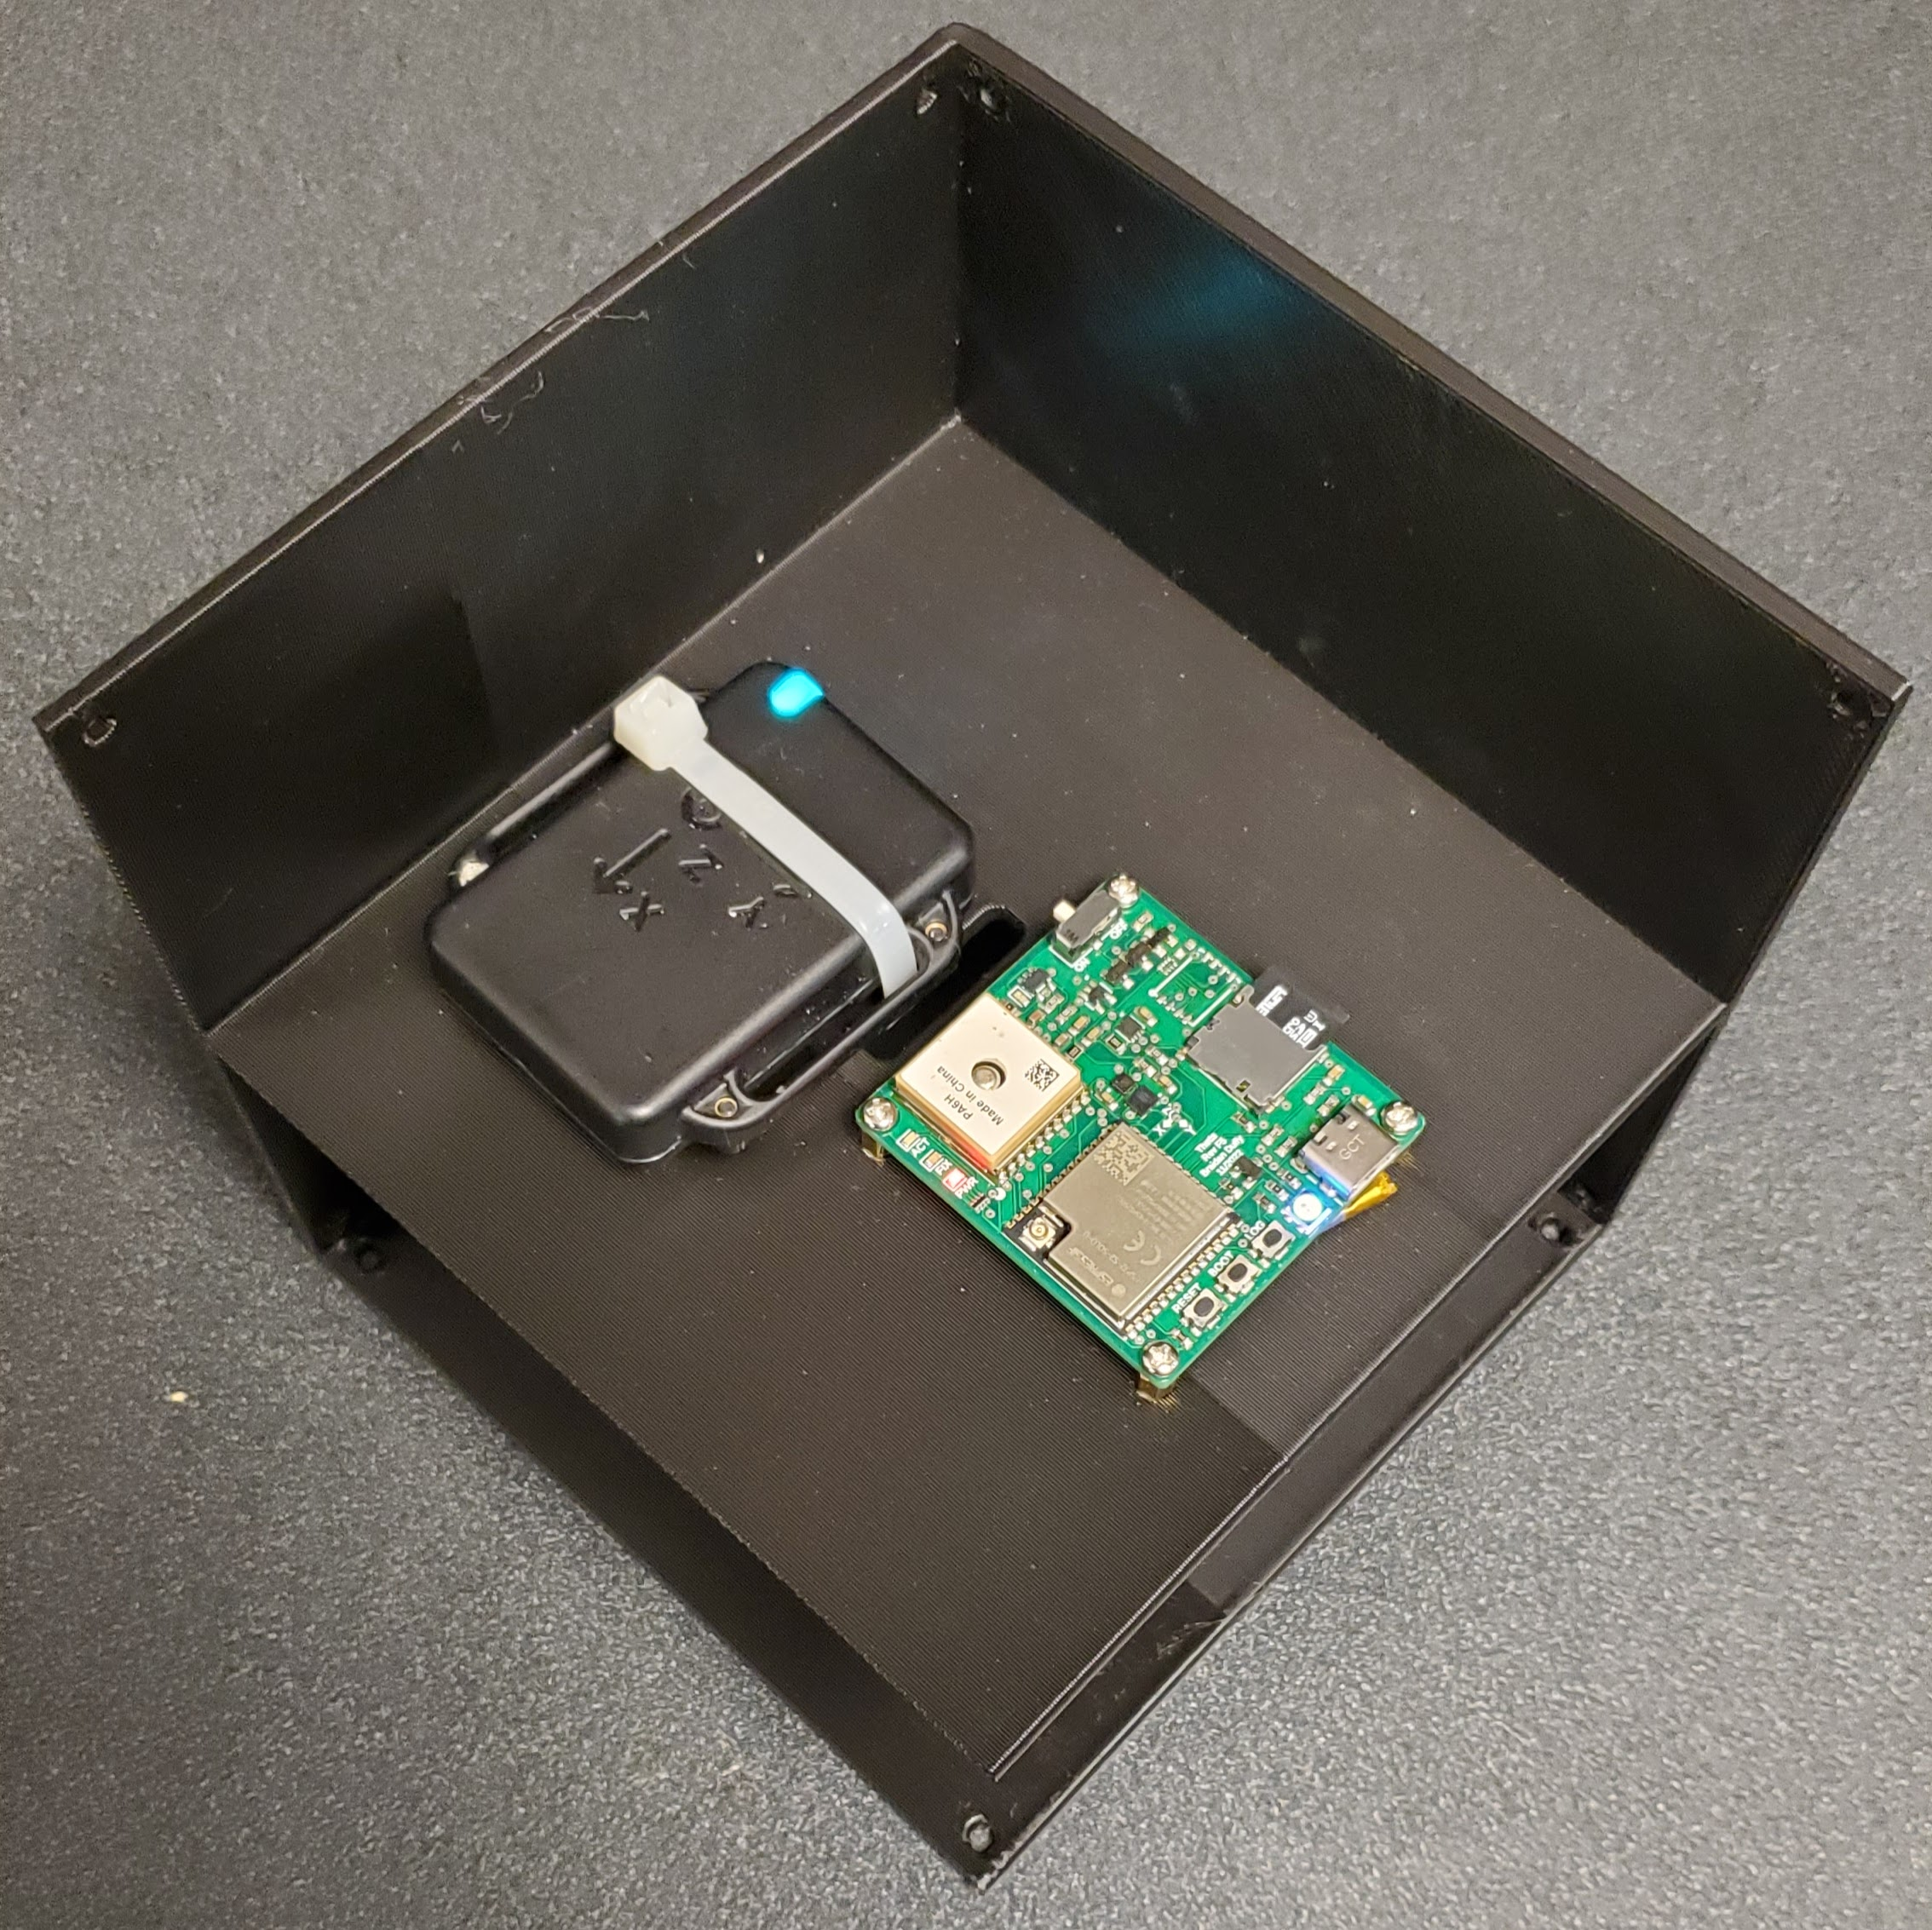
\includegraphics[height=2in]{calibration/calibration_cube2.jpg}
%     \caption[Calibration cube]{}
%     \labfig{calibration_cube}
% \end{figure}

To test the accelerometer and orientation data, a 72-tooth gear and socket was cut out of spare wood using a laser cutter.
With 72 teeth, the gear has a rotational resolution of 5-degrees per tooth with high precision as the laser cut did not leave any room for play between the gear and socket.

% \begin{figure}[h!]
%     \centering
%     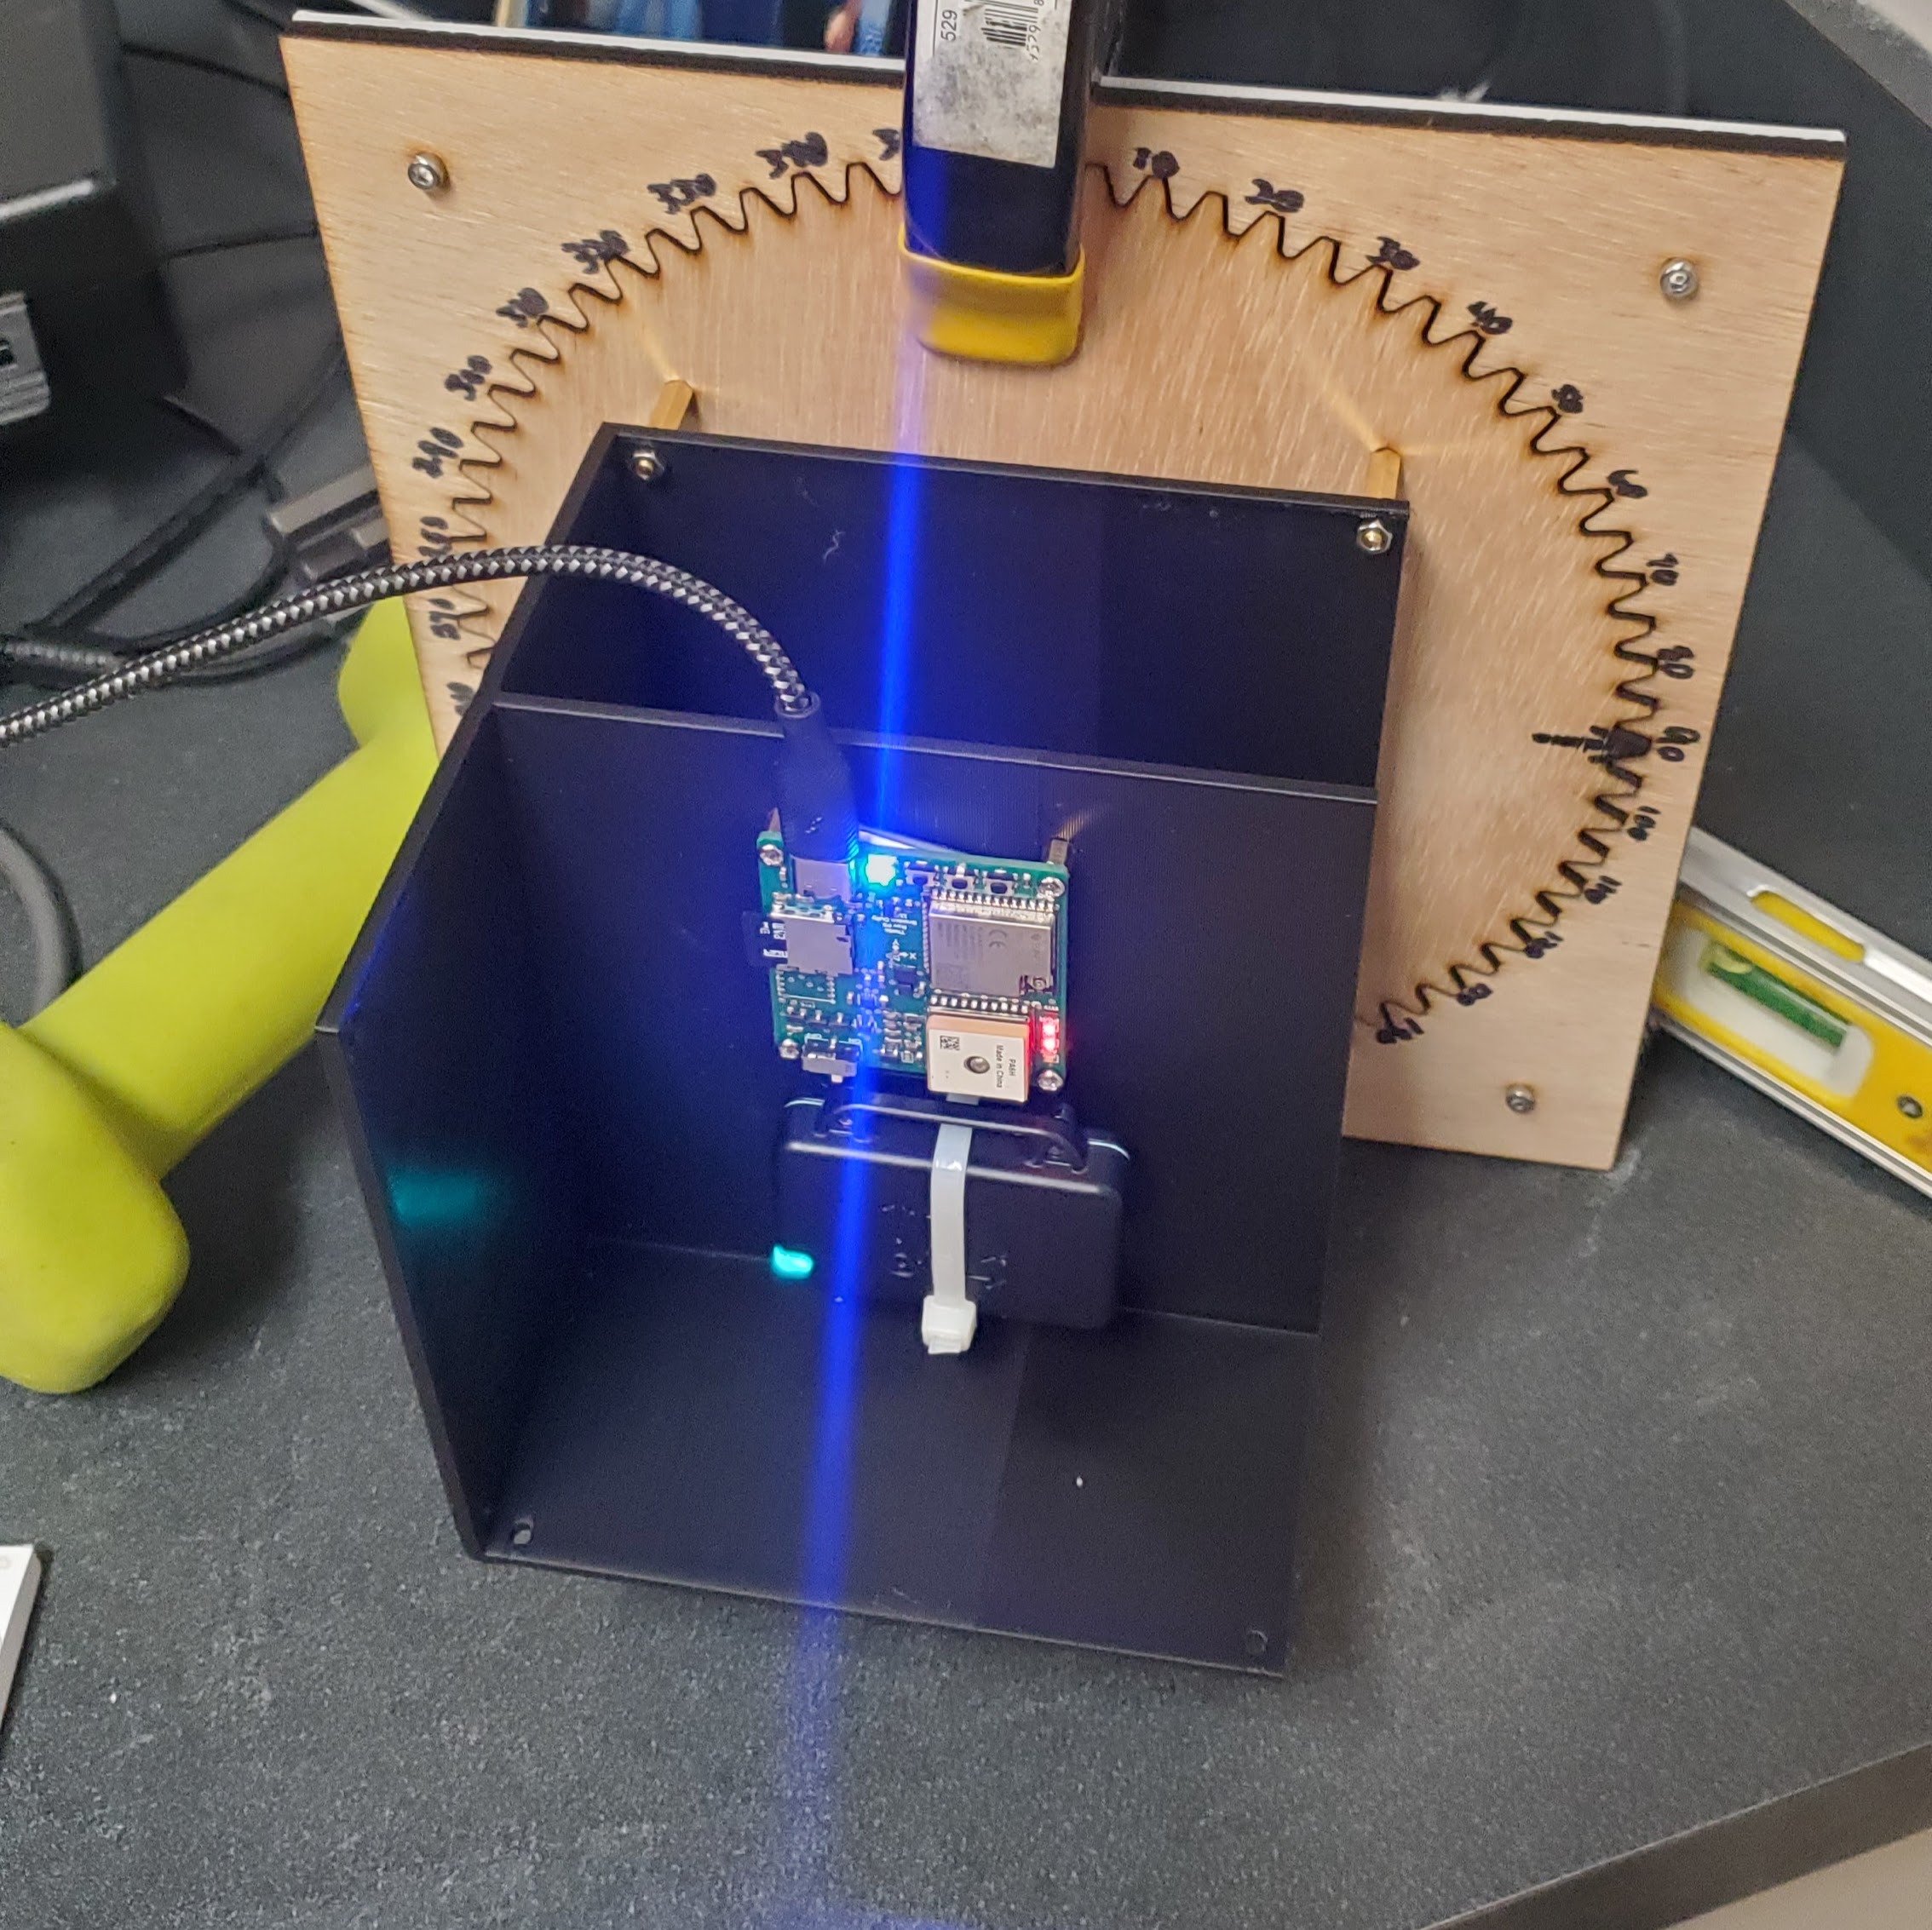
\includegraphics[height=2in]{calibration/calibration_cube_gear.jpg}
%     \caption[Calibration cube with gear and socket]{Calibration cube mounted in the gear and socket apparatus for accelerometer and orientation testing.}
%     \labfig{calibration_cube_gear}
% \end{figure}

Finally, to test the gyroscope, a machine was designed and created that could rotate the calibration cube at a constant specified rate.
It is built around a Raspberry Pi running Robot Operating System 2 \cite{Macenski:2022} using a stepper motor driver HAT\footnote{\url{https://www.waveshare.com/stepper-motor-hat.htm}}.
The HAT is connected to a stepper motor which is coupled to a plate mounted on a lazy susan bearing\footnote{\url{https://www.tindie.com/products/fluxgarage/turntable-for-stepper-motor-kit/}}.
Commands to the Pi allow it to start the motor, begin rotating, and then stop rotating.
Some other features are implemented, but not used for calibration.

% \begin{figure}[h!]
%     \centering
%     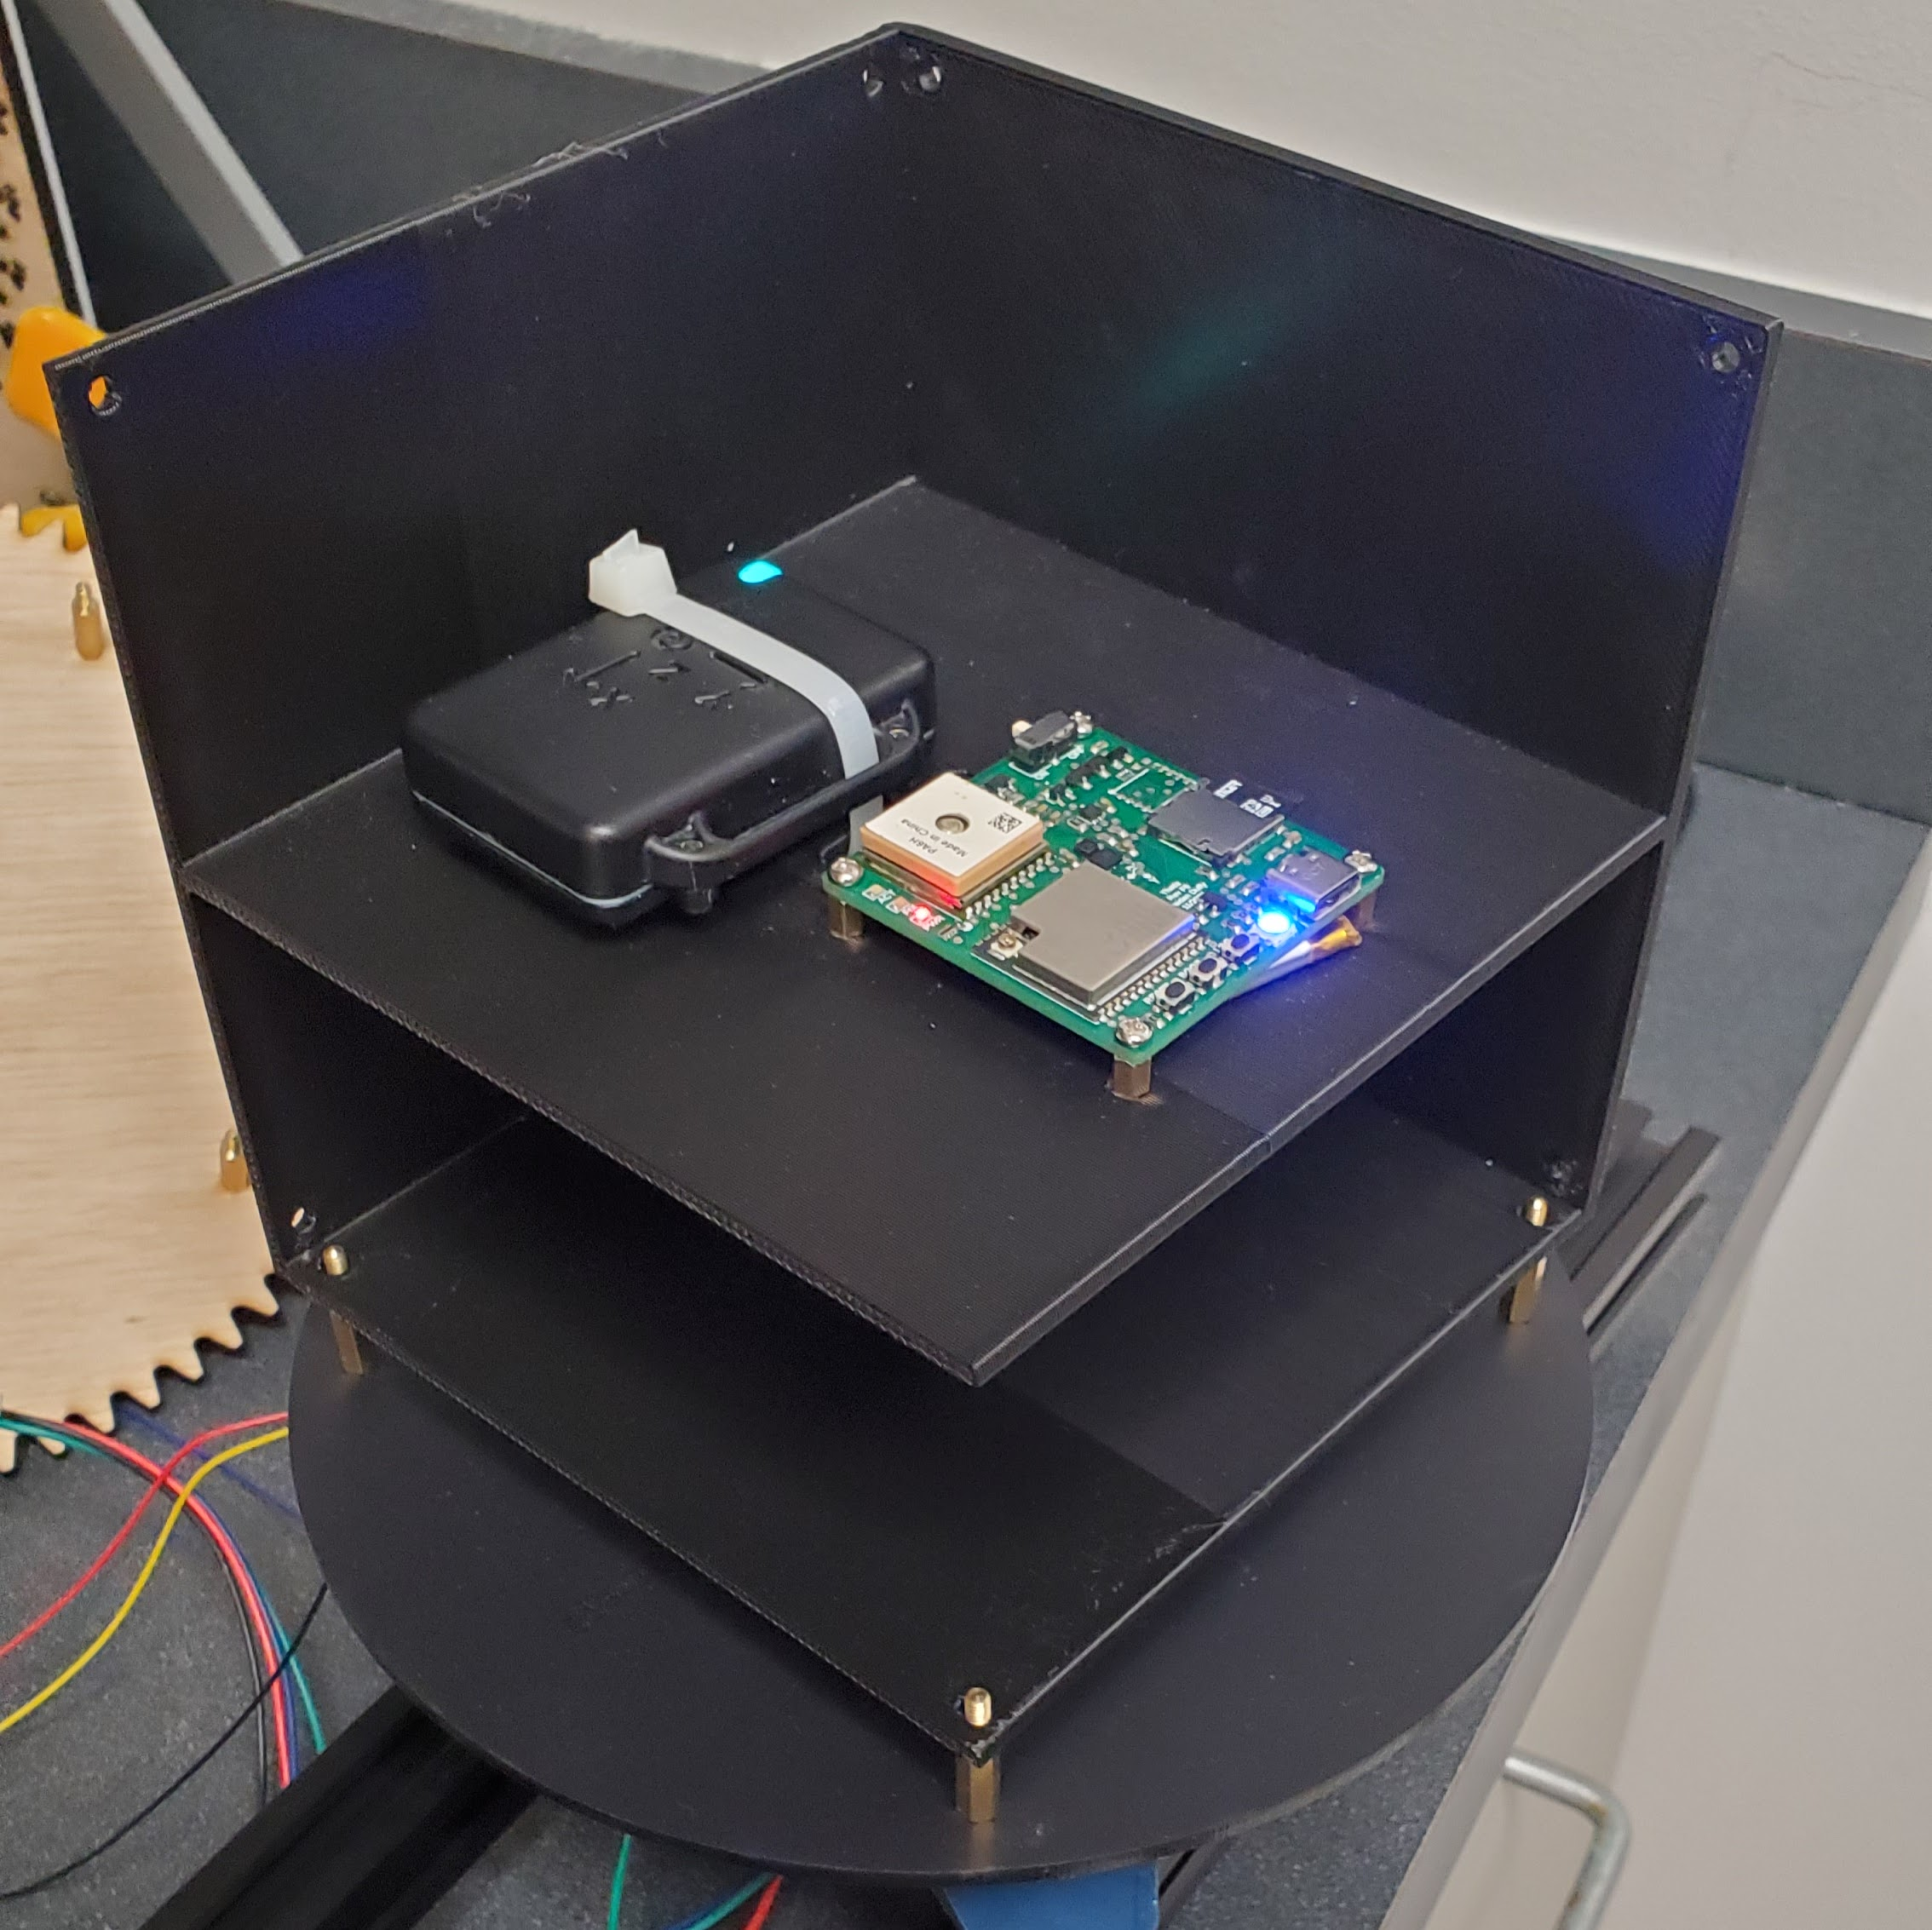
\includegraphics[height=2in]{calibration/calibration_cube_machine.jpg}
%     \caption[Calibration cube on a rotating plate]{Calibration cube mounted on top of the rotating plate for gyroscope data collection.}
%     \labfig{calibration_cube_machine}
% \end{figure}

\begin{figure}[h!]
    \centering
    \subfloat[Calibration cube with the x-IMU3 (left) and Thetis (right) mounted on it]{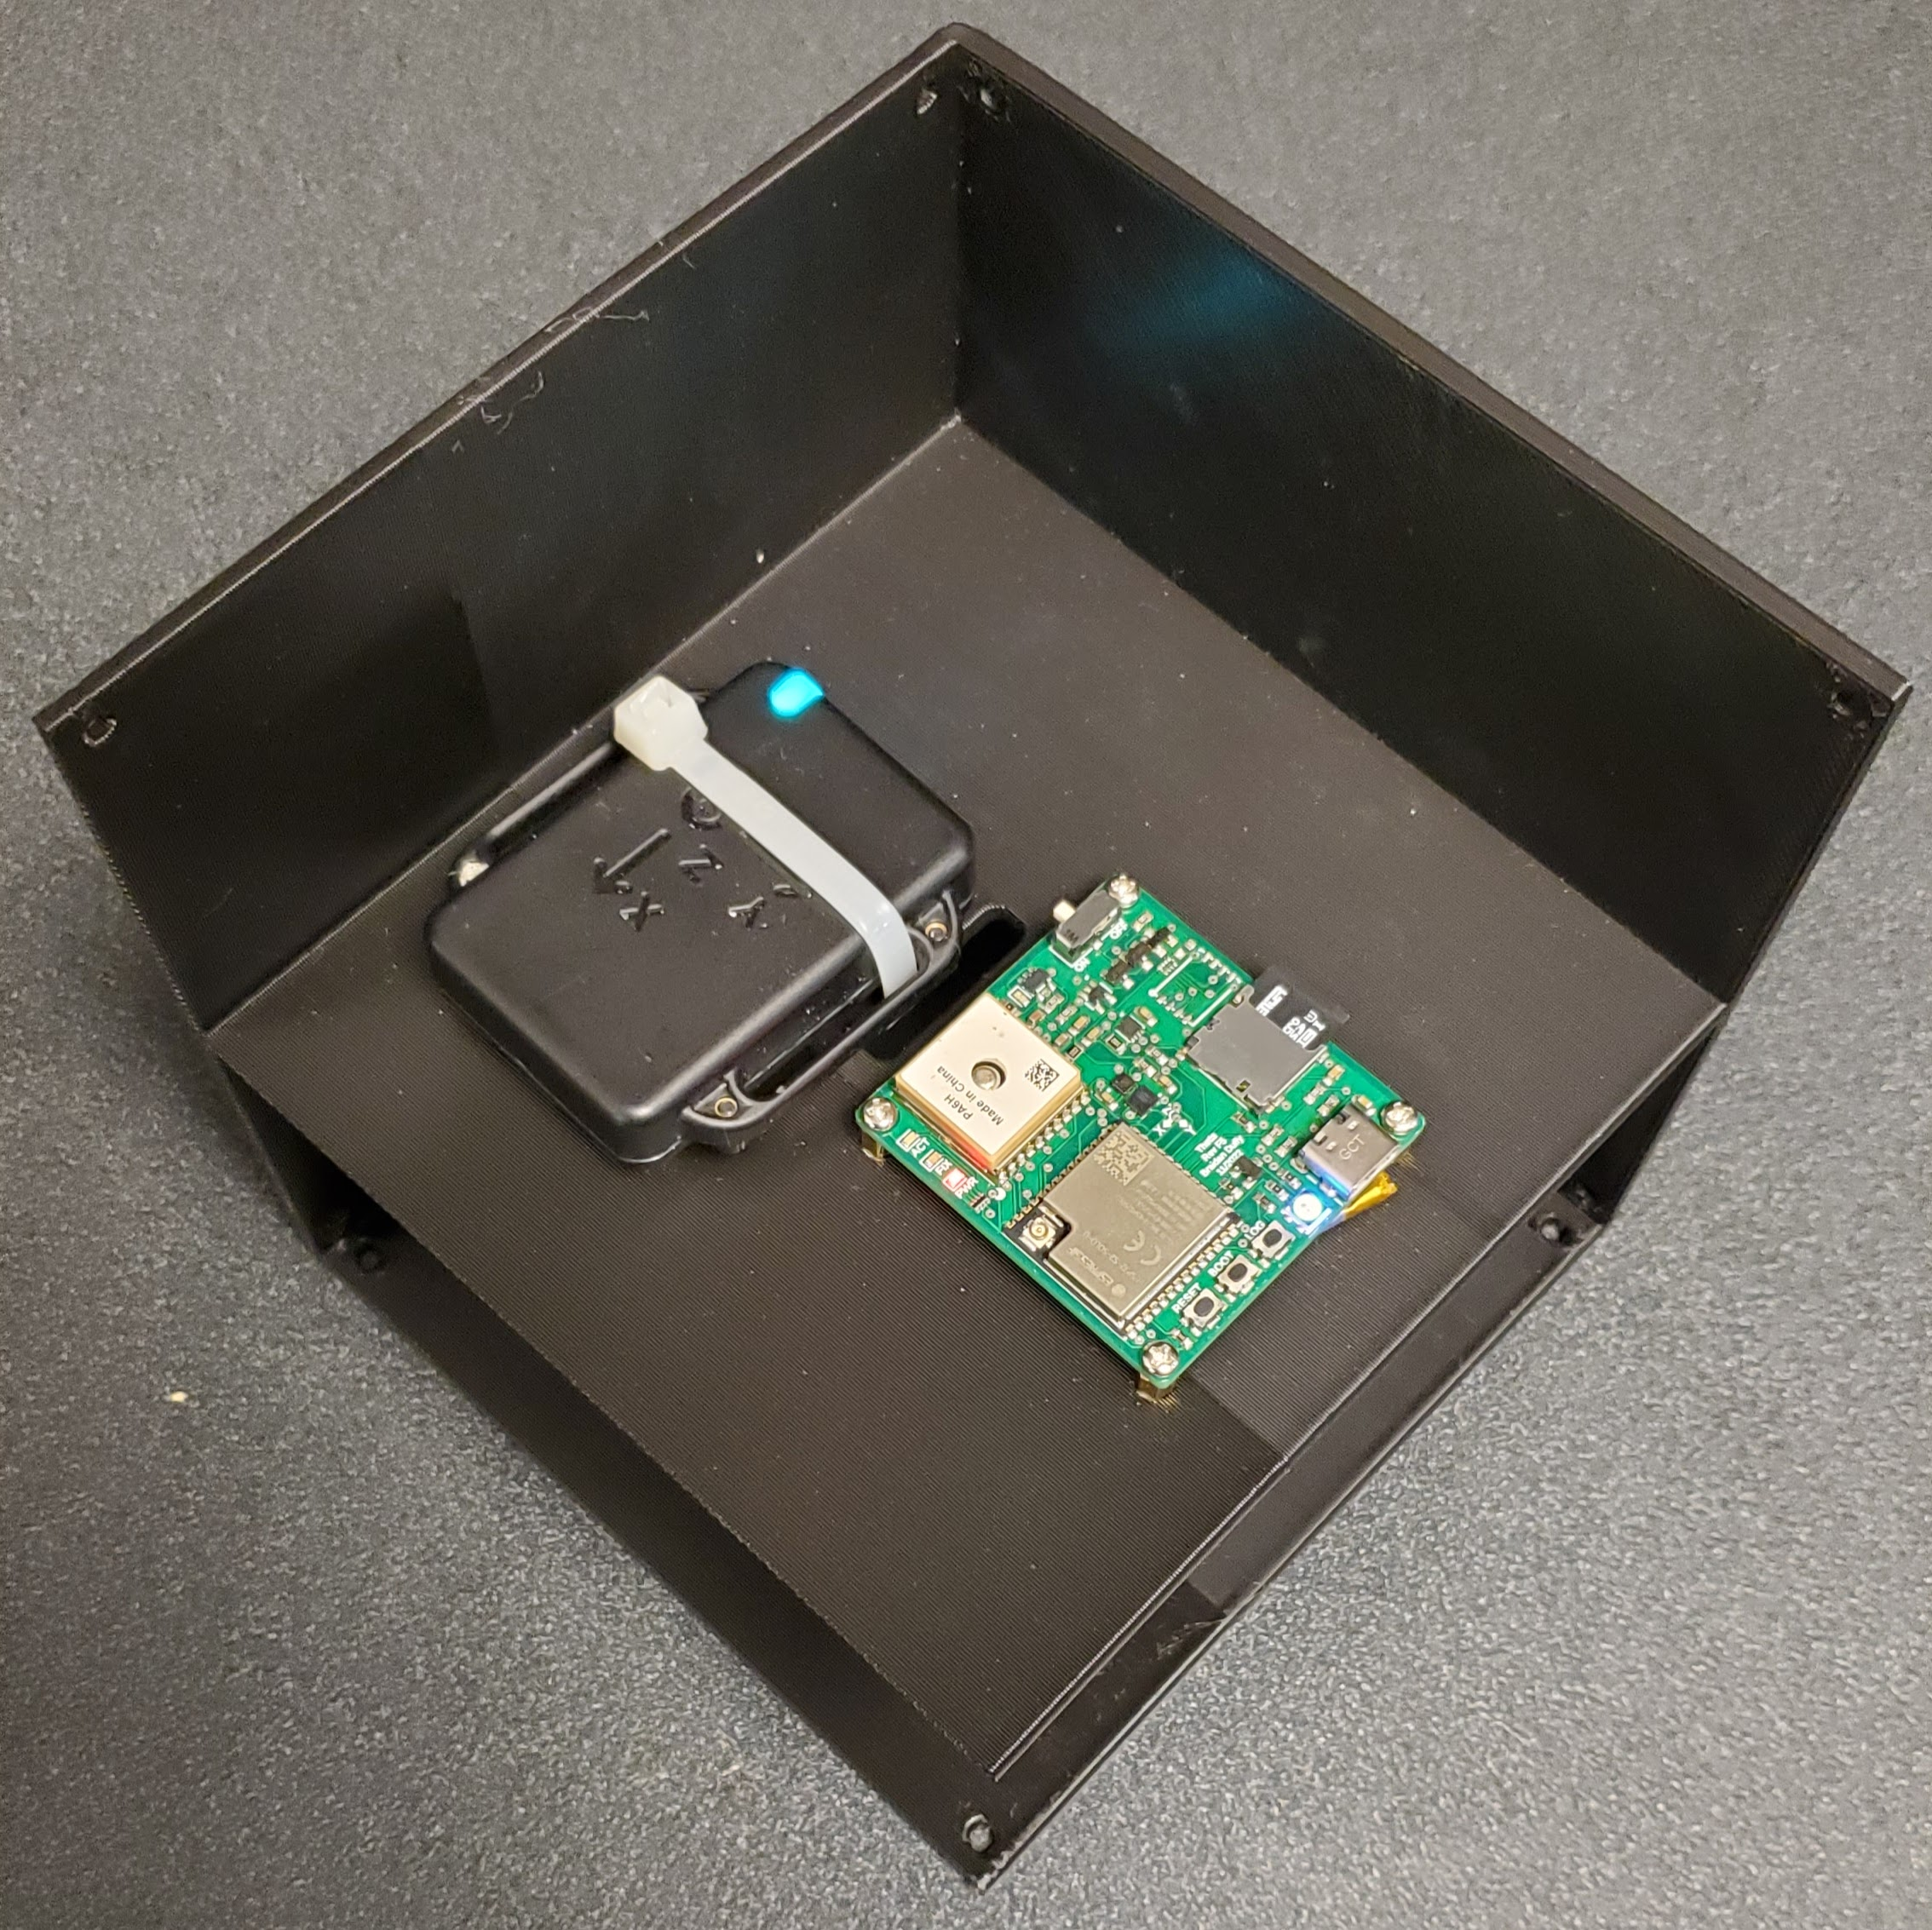
\includegraphics[width=0.3\textwidth]{calibration/calibration_cube2.jpg}\label{subfig:calibration_cube}}\hskip3ex
    \subfloat[Calibration cube mounted in the gear and socket apparatus for accelerometer and orientation testing.]{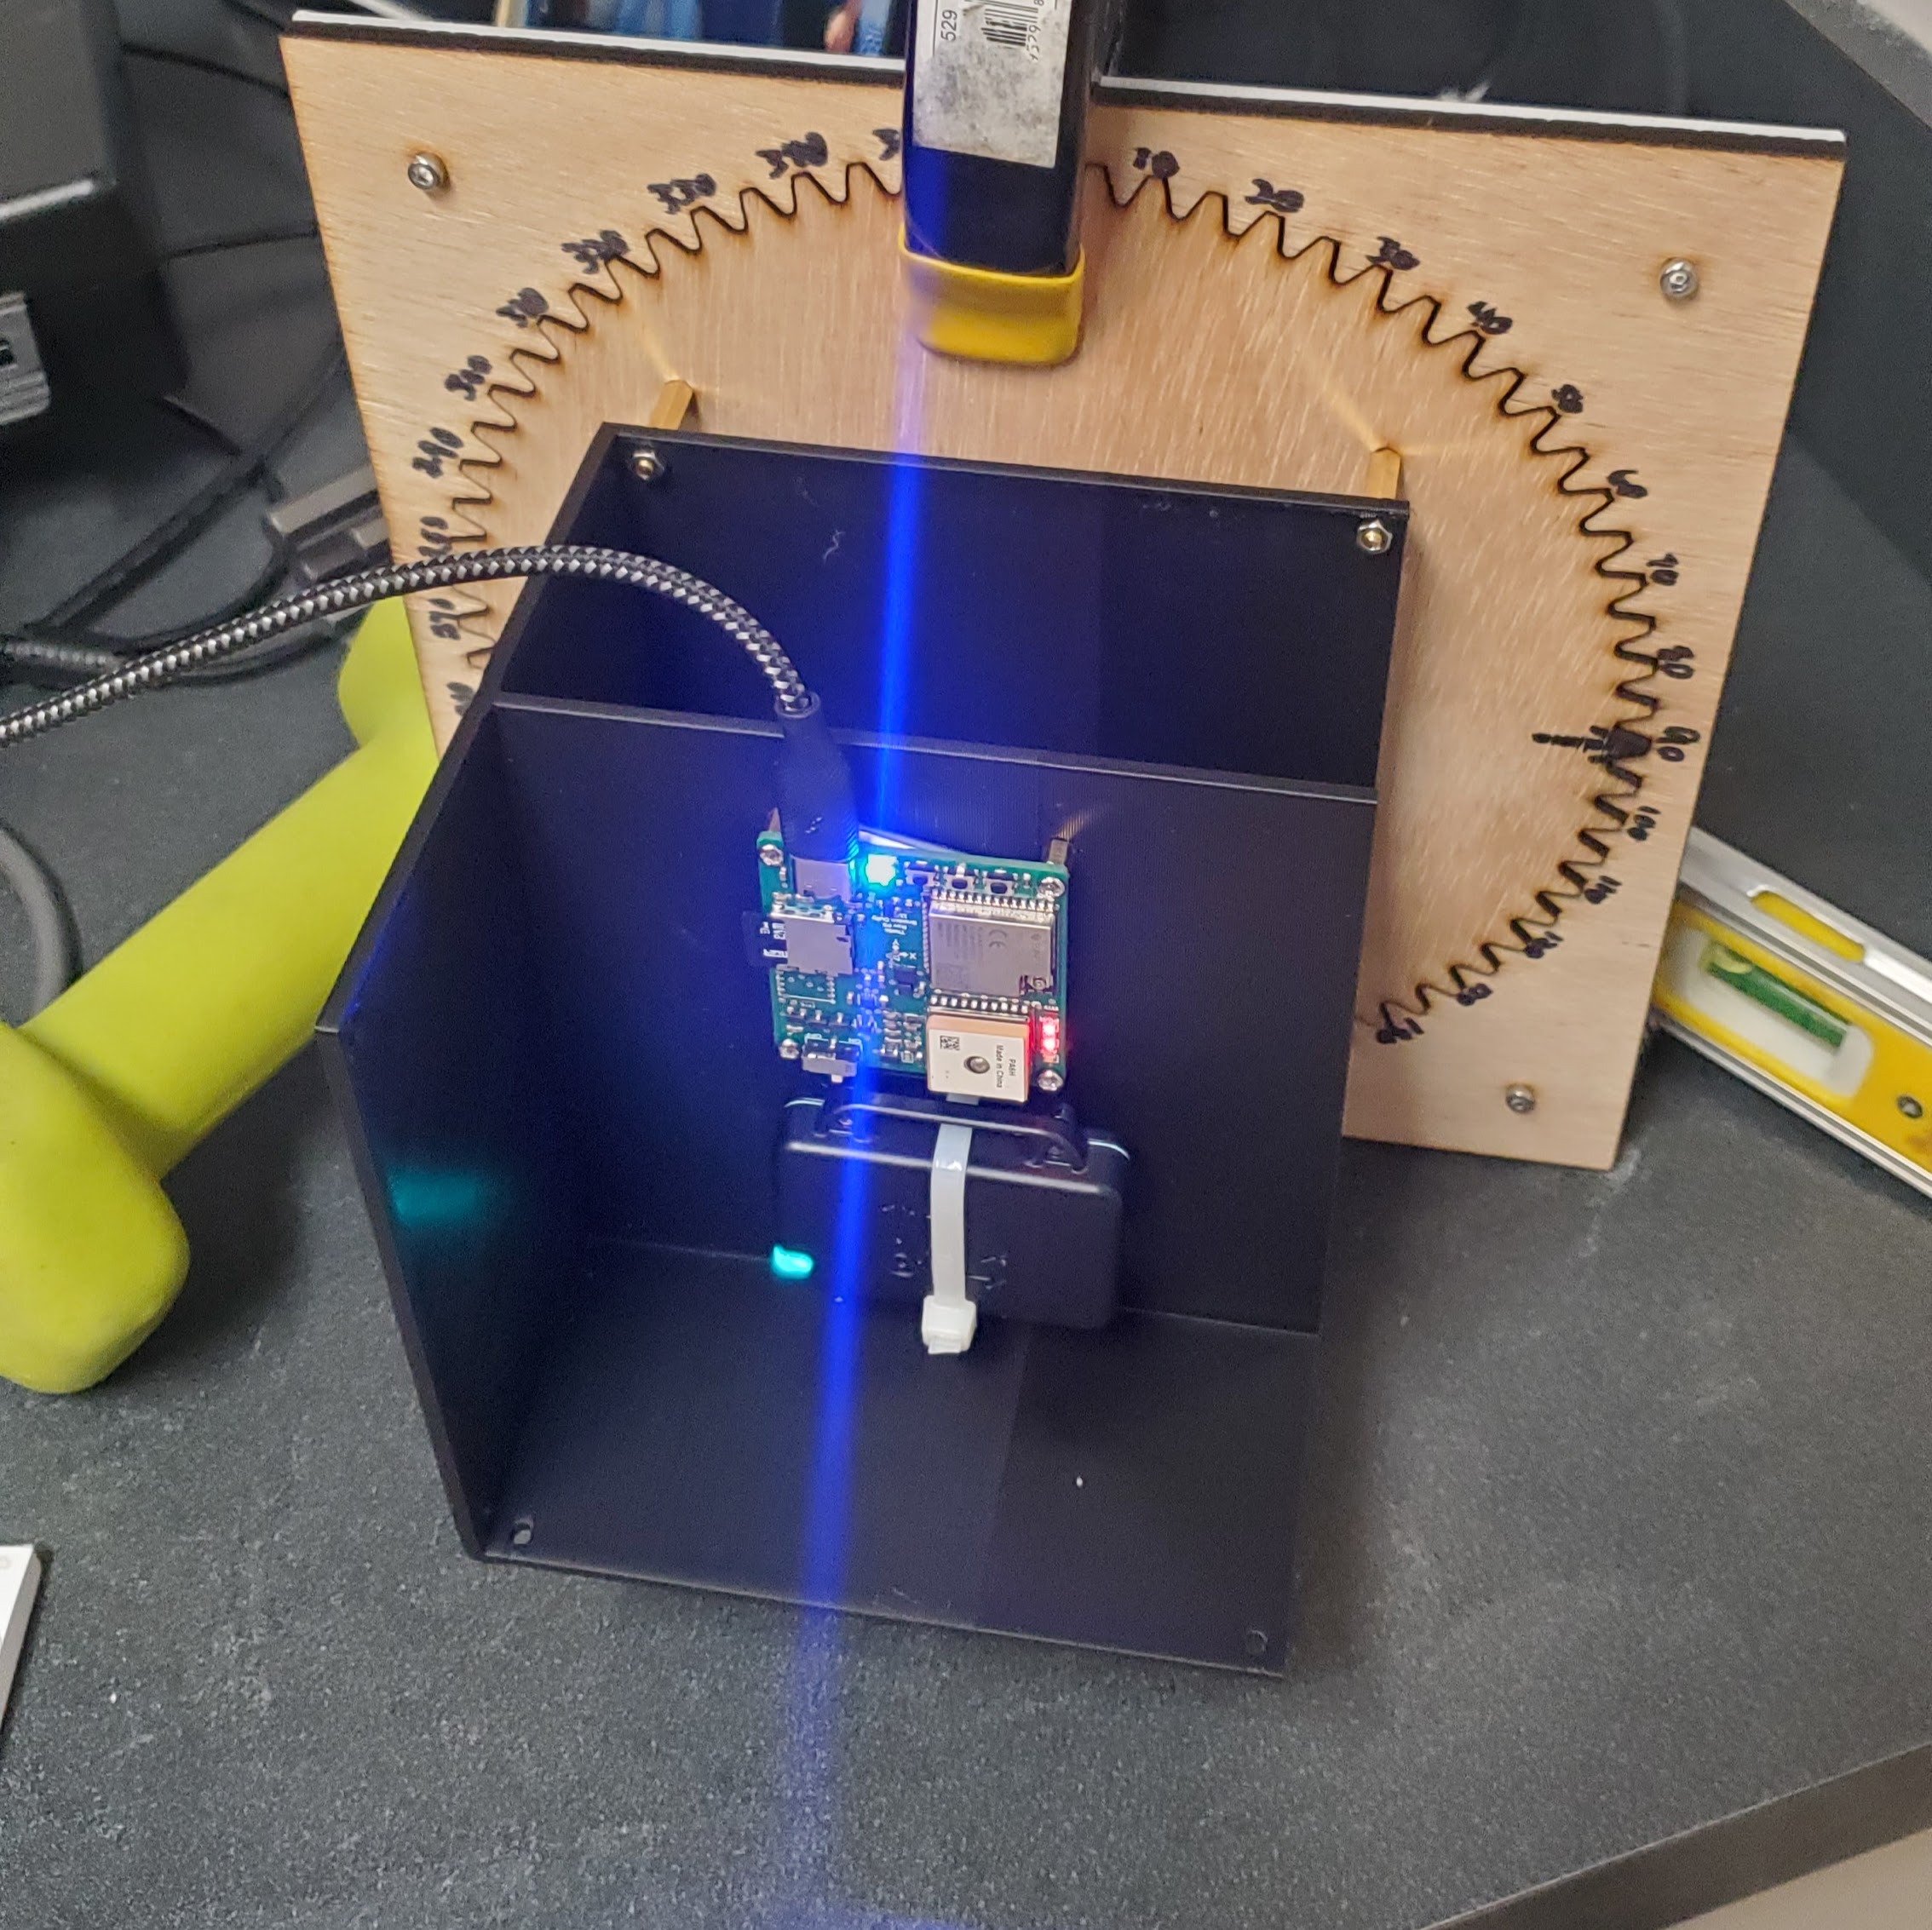
\includegraphics[width=0.3\textwidth]{calibration/calibration_cube_gear.jpg}\label{subfig:calibration_cube_gear}}\hskip3ex
    \subfloat[Calibration cube mounted on top of the rotating plate for gyroscope data collection.]{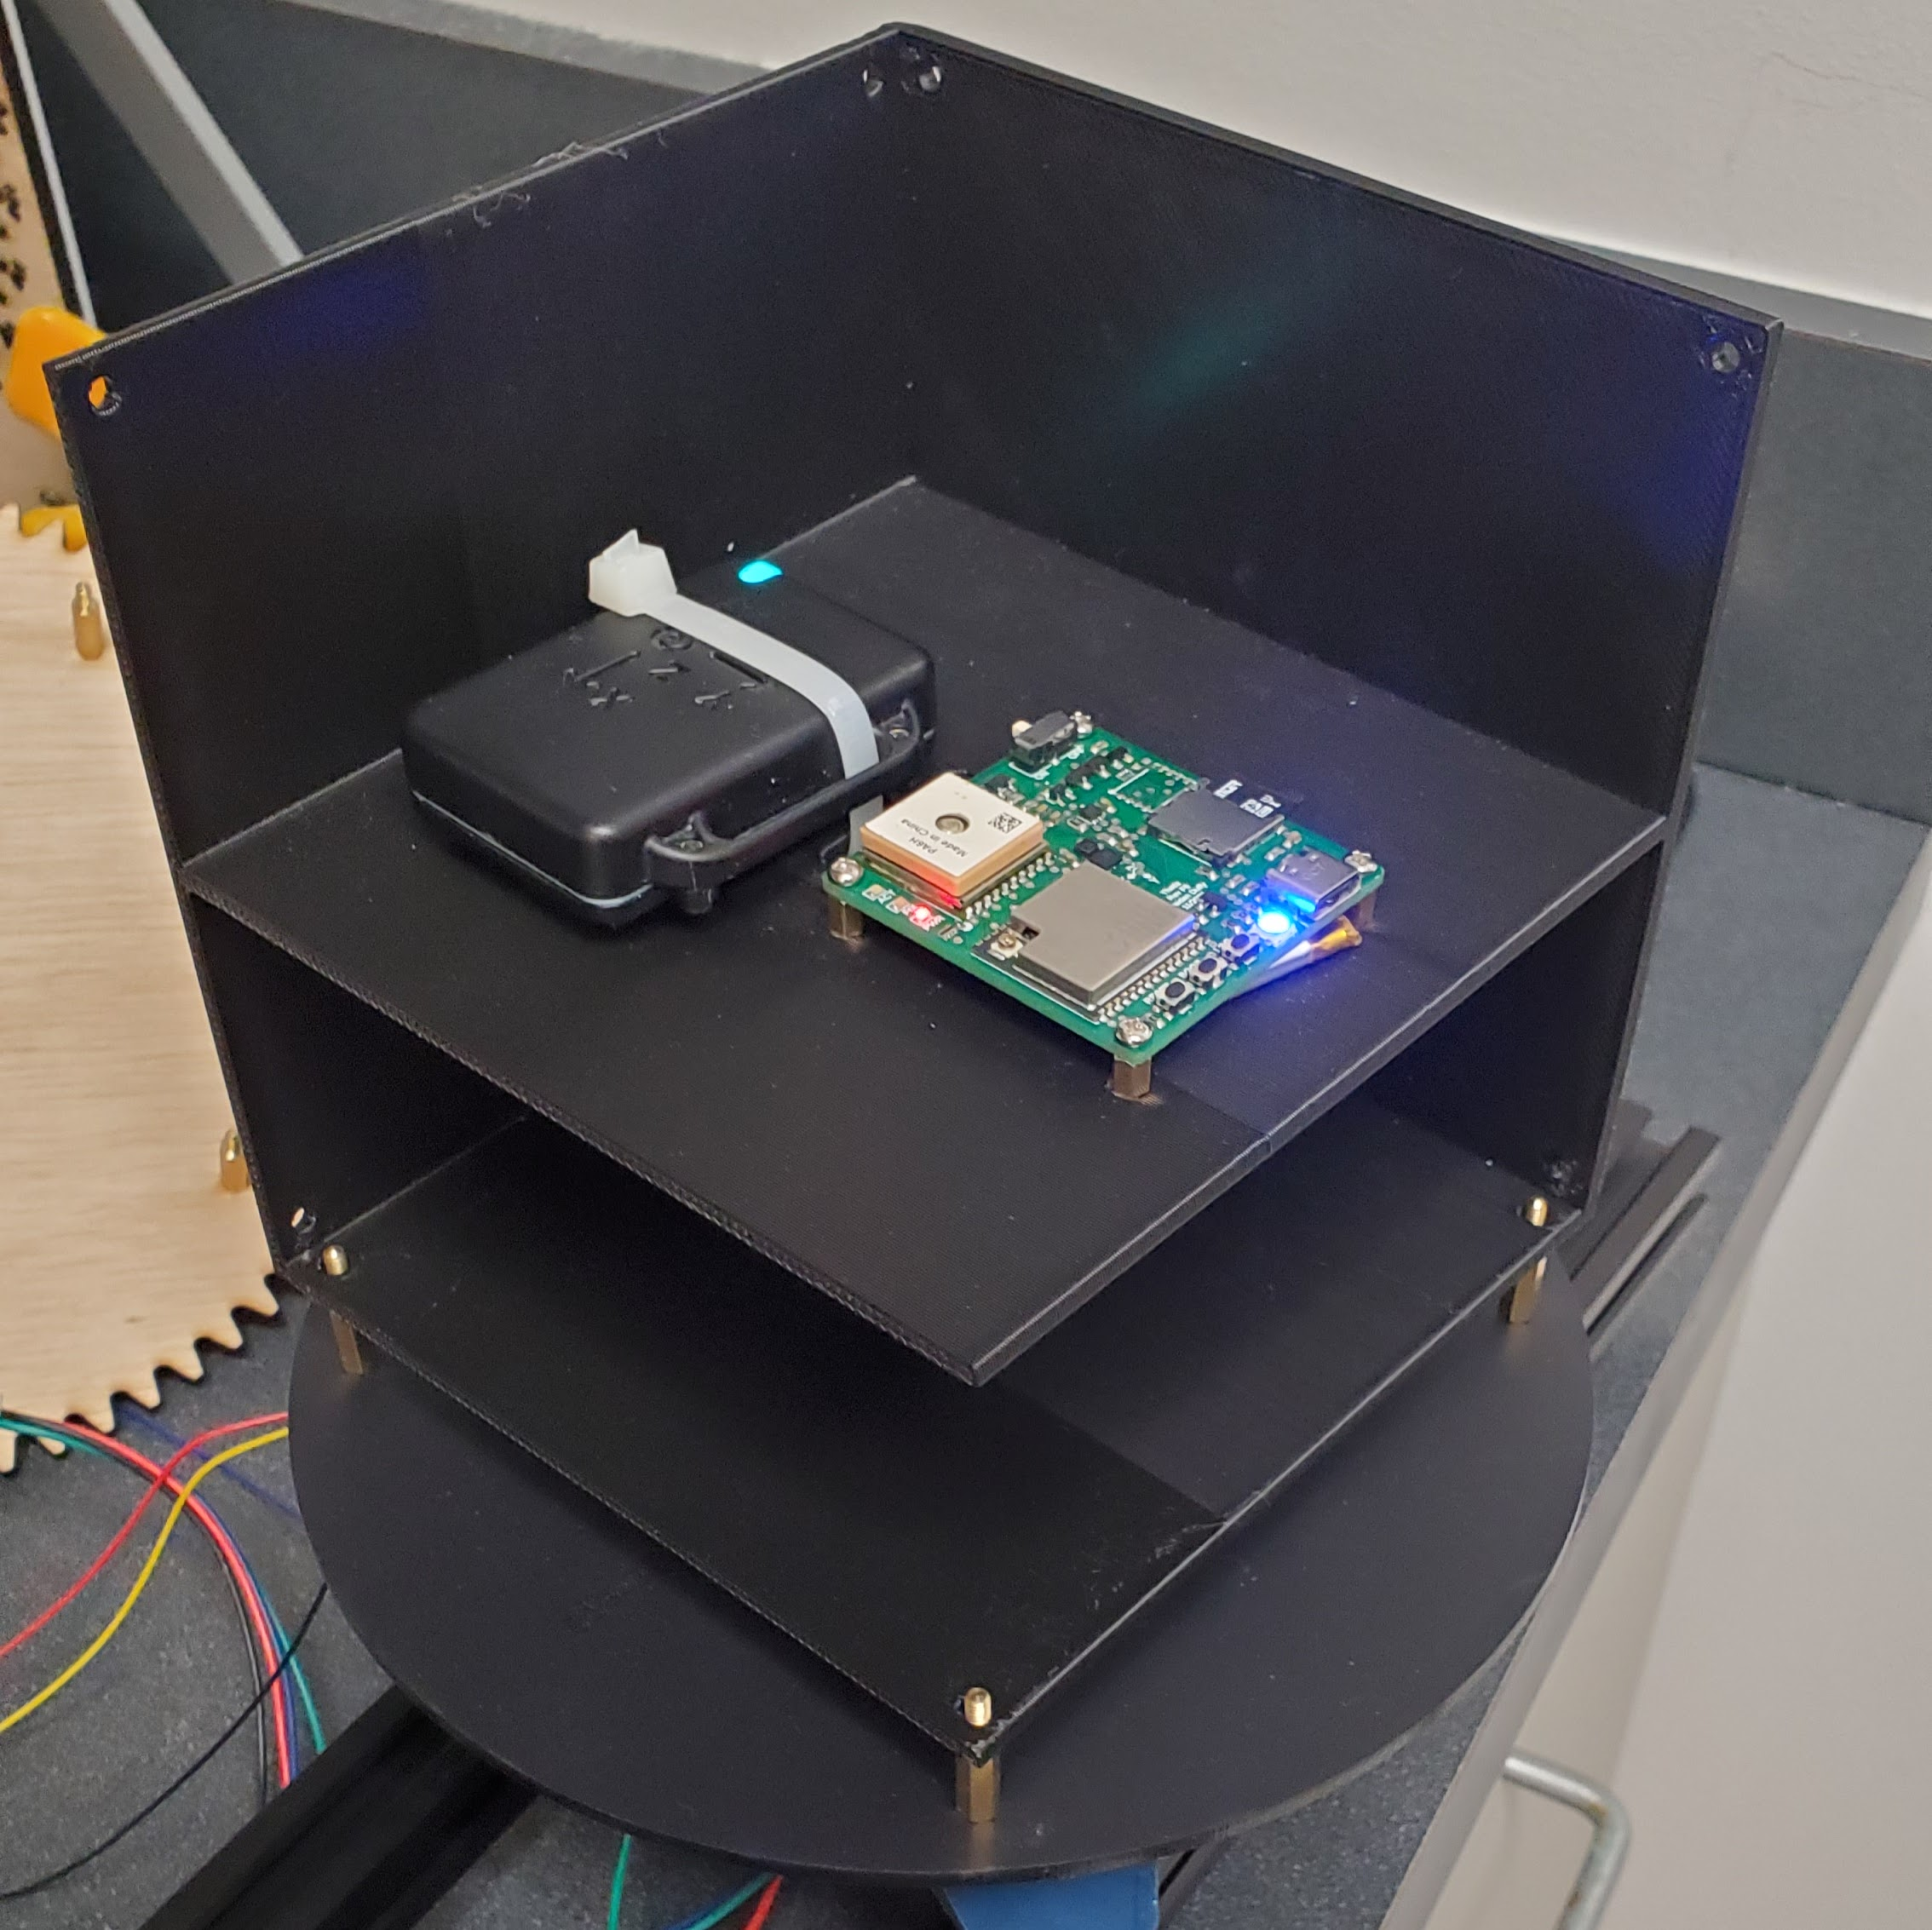
\includegraphics[width=0.3\textwidth]{calibration/calibration_cube_machine.jpg}\label{subfig:calibration_cube_machine}}
	\caption[Calibration apparatuses]{The different tools designed and used for calibration Thetis}
	\labfig{calibration_tools}
\end{figure}

\section{Methodologies} \labsec{calibration_methodologies}
The calibration process is important to improve the accuracy of the sensor before post processing and analysis are performed.
It is crucial that the calibration parameter settings on the device are at their default values before beginning.
Each of the starting misalignment ($M_0$), soft iron ($W^{-1}_0$), and sensitivity ($S_0$) matrices should be 3 $\times$ 3 identity matrices and the starting bias ($\pmb{b}_0$) and hard iron vectors ($\pmb{v}_0$) should be zero vectors.

\begin{gather}
    \begin{aligned}
        M_0 &= 
        \begin{bmatrix}
        1 & 0 & 0 \\
        0 & 1 & 0 \\
        0 & 0 & 1 \\    
        \end{bmatrix} \\
        W^{-1}_0 &= 
        \begin{bmatrix}
            1 & 0 & 0 \\
            0 & 1 & 0 \\
            0 & 0 & 1 \\    
        \end{bmatrix} \\
        S_0 &= 
        \begin{bmatrix}
            1 & 0 & 0 \\
            0 & 1 & 0 \\
            0 & 0 & 1 \\
        \end{bmatrix} \\
        \pmb{b}_0 &= 
        \begin{bmatrix}
            0 & 0 & 0
        \end{bmatrix} \\
        \pmb{v}_0 &= 
        \begin{bmatrix}
            0 & 0 & 0
        \end{bmatrix}
    \end{aligned} \notag
\end{gather}

\subsection{Magnetometer} \labsubsec{calibration_magnetometer}
To calibrate the magnetometer, it needs to be rotated about all three axes in a ``figure-8'' motion.
This can be best accomplished by rotating about a point while making the figure-8 pattern.
This ensures that the measurements in the x-, y-, and z-axis are evenly distributed throughout the magnetic field.
Without any distortions, this will create a sphere with a radius of the magnitude of the magnetic field.
However, as discussed in Chapter \ref{chap:background} and evidenced in Section \ref{sec:calibration_results}, this is not always the case.
To improve accuracy, the entire apparatus should be far away from any magnetic influences such as electrical fields and permanent magnets.

\subsection{Gyroscope} \labsubsec{calibration_gyroscope}
The gyroscope is calibrated using the calibration machine discussed more in Appendix \ref{chap:calibration_machine_design}. 
To begin, the machine must be booted and the measurement devices turned on.
Then, two terminal windows can be opened on the machine's Raspberry Pi through SSH or a headed setup.
On one terminal, navigate to the \lstinline[style=customInline]|calibrator_ws/| directory and execute the following command:

\begin{bash}
    source install/setup.bash && ros2 launch calibrator_bringup plate.launch.py
\end{bash}

\noindent This will start the ROS2 environment and allow the user to run the motor using the command line interface (CLI).
Ensure that the calibration machine is flat and level with the rotating plate horizontal as shown in Figure \ref{subfig:calibration_cube_machine}.
When ready, set up the test by specifying the motor direction and speed in the second terminal window.
The former can be set using the command:

\begin{bash}
    ros2 service call /set_motor_dir calibrator_interfaces/SetBool "{data: DIR}"
\end{bash}

\noindent Where \lstinline[style=customInline]|DIR| is the desired direction - \lstinline[style=customInline]|true| will set the motor direction to clockwise, \lstinline[style=customInline]|false| will set the motor direction to counter-clockwise.
The motor speed can be set with the command:

\begin{bash}
    ros2 service call /set_motor_speed calibrator_interfaces/SetFloat64 "{data: SPEED}"
\end{bash}

\noindent Where \lstinline[style=customInline]|SPEED| is the desired test speed in degrees per second.
Note that it is not accurate and needs to be checked using an external tachometer.
For reference, calibration was done using three settings: 200, 300, and 400 which corresponded with the tachometer measurements of 305 deg/sec, 410 deg/sec, and 500 deg/sec, respectively.
To start the motor spinning, execute the command:

\begin{bash}
    ros2 service call /start_motor std_srvs/Trigger
\end{bash}

\noindent After a moment, the plate will begin spinning at the specified speed and direction.
Once you have collected the data, you can stop the motor using the command:

\begin{bash}
    ros2 service call /stop_motor std_srvs/Trigger
\end{bash}

\noindent After a few moments, the motor will come to a stop and the data can be offloaded.
Note that this command resets the motor speed to a default value, so you will need to set the speed using the commands again.
It will be beneficial to start/stop recording at the start and end of every test so that a single log file represents a single test.

\subsection{Accelerometer} \labsubsec{calibration_accelerometer}
The accelerometer must be calibrated on the gear and socket apparatus while it is vertical.
The apparatus should be leveled such that the instruments on the calibration cube are perfectly vertical with respect to gravity and the other axes are planar to the Earth's surface.
Choose an axis and place the positive direction downwards (-1g).
The arrows on the coordinate reference markers on each device point towards the positive direction.
Then, align the indicator on the gear with 0-degree marker on the socket, as shown in Figure \ref{subfig:calibration_cube_gear}.

Rotate the calibration cube and gear in 45-degree increments, stopping for 30-seconds at each interval to collect an good average of data.
It will be beneficial to start/stop recording at the start and end of each increment so that a single log file represents a single orientation.

\subsection{Orientation} \labsubsec{calibration_orientation}
Roll and pitch orientation data can be collected simultaneously with the accelerometer calibration data as the devices are rotated about the x- and y-axis, respectively.
This will give roll and pitch in 45-degree increments that can be analyzed for errors before and after calibration.

To get the yaw readings, we can re-use the gear and socket apparatus, this time placing it flat on a surface and placing the z-axis of the devices vertical.
Make sure that the entire apparatus is far away from any magnetic influences and near the location where the magnetometer was calibrated.
Start the gear at the 0-degree marker on the socket, then orient the entire apparatus to magnetic north as determined by an external compass as shown in Figure \ref{fig:calibration_cube_compass}.
Rotate the calibration cube and gear in 45-degree increments for 360-degrees, pausing for 30-seconds at each interval to get an average reading.
It will be beneficial to start/stop recording at the start and end of each increment so that a single log file represents a single orientation.

\begin{figure}[h!]
    \centering
    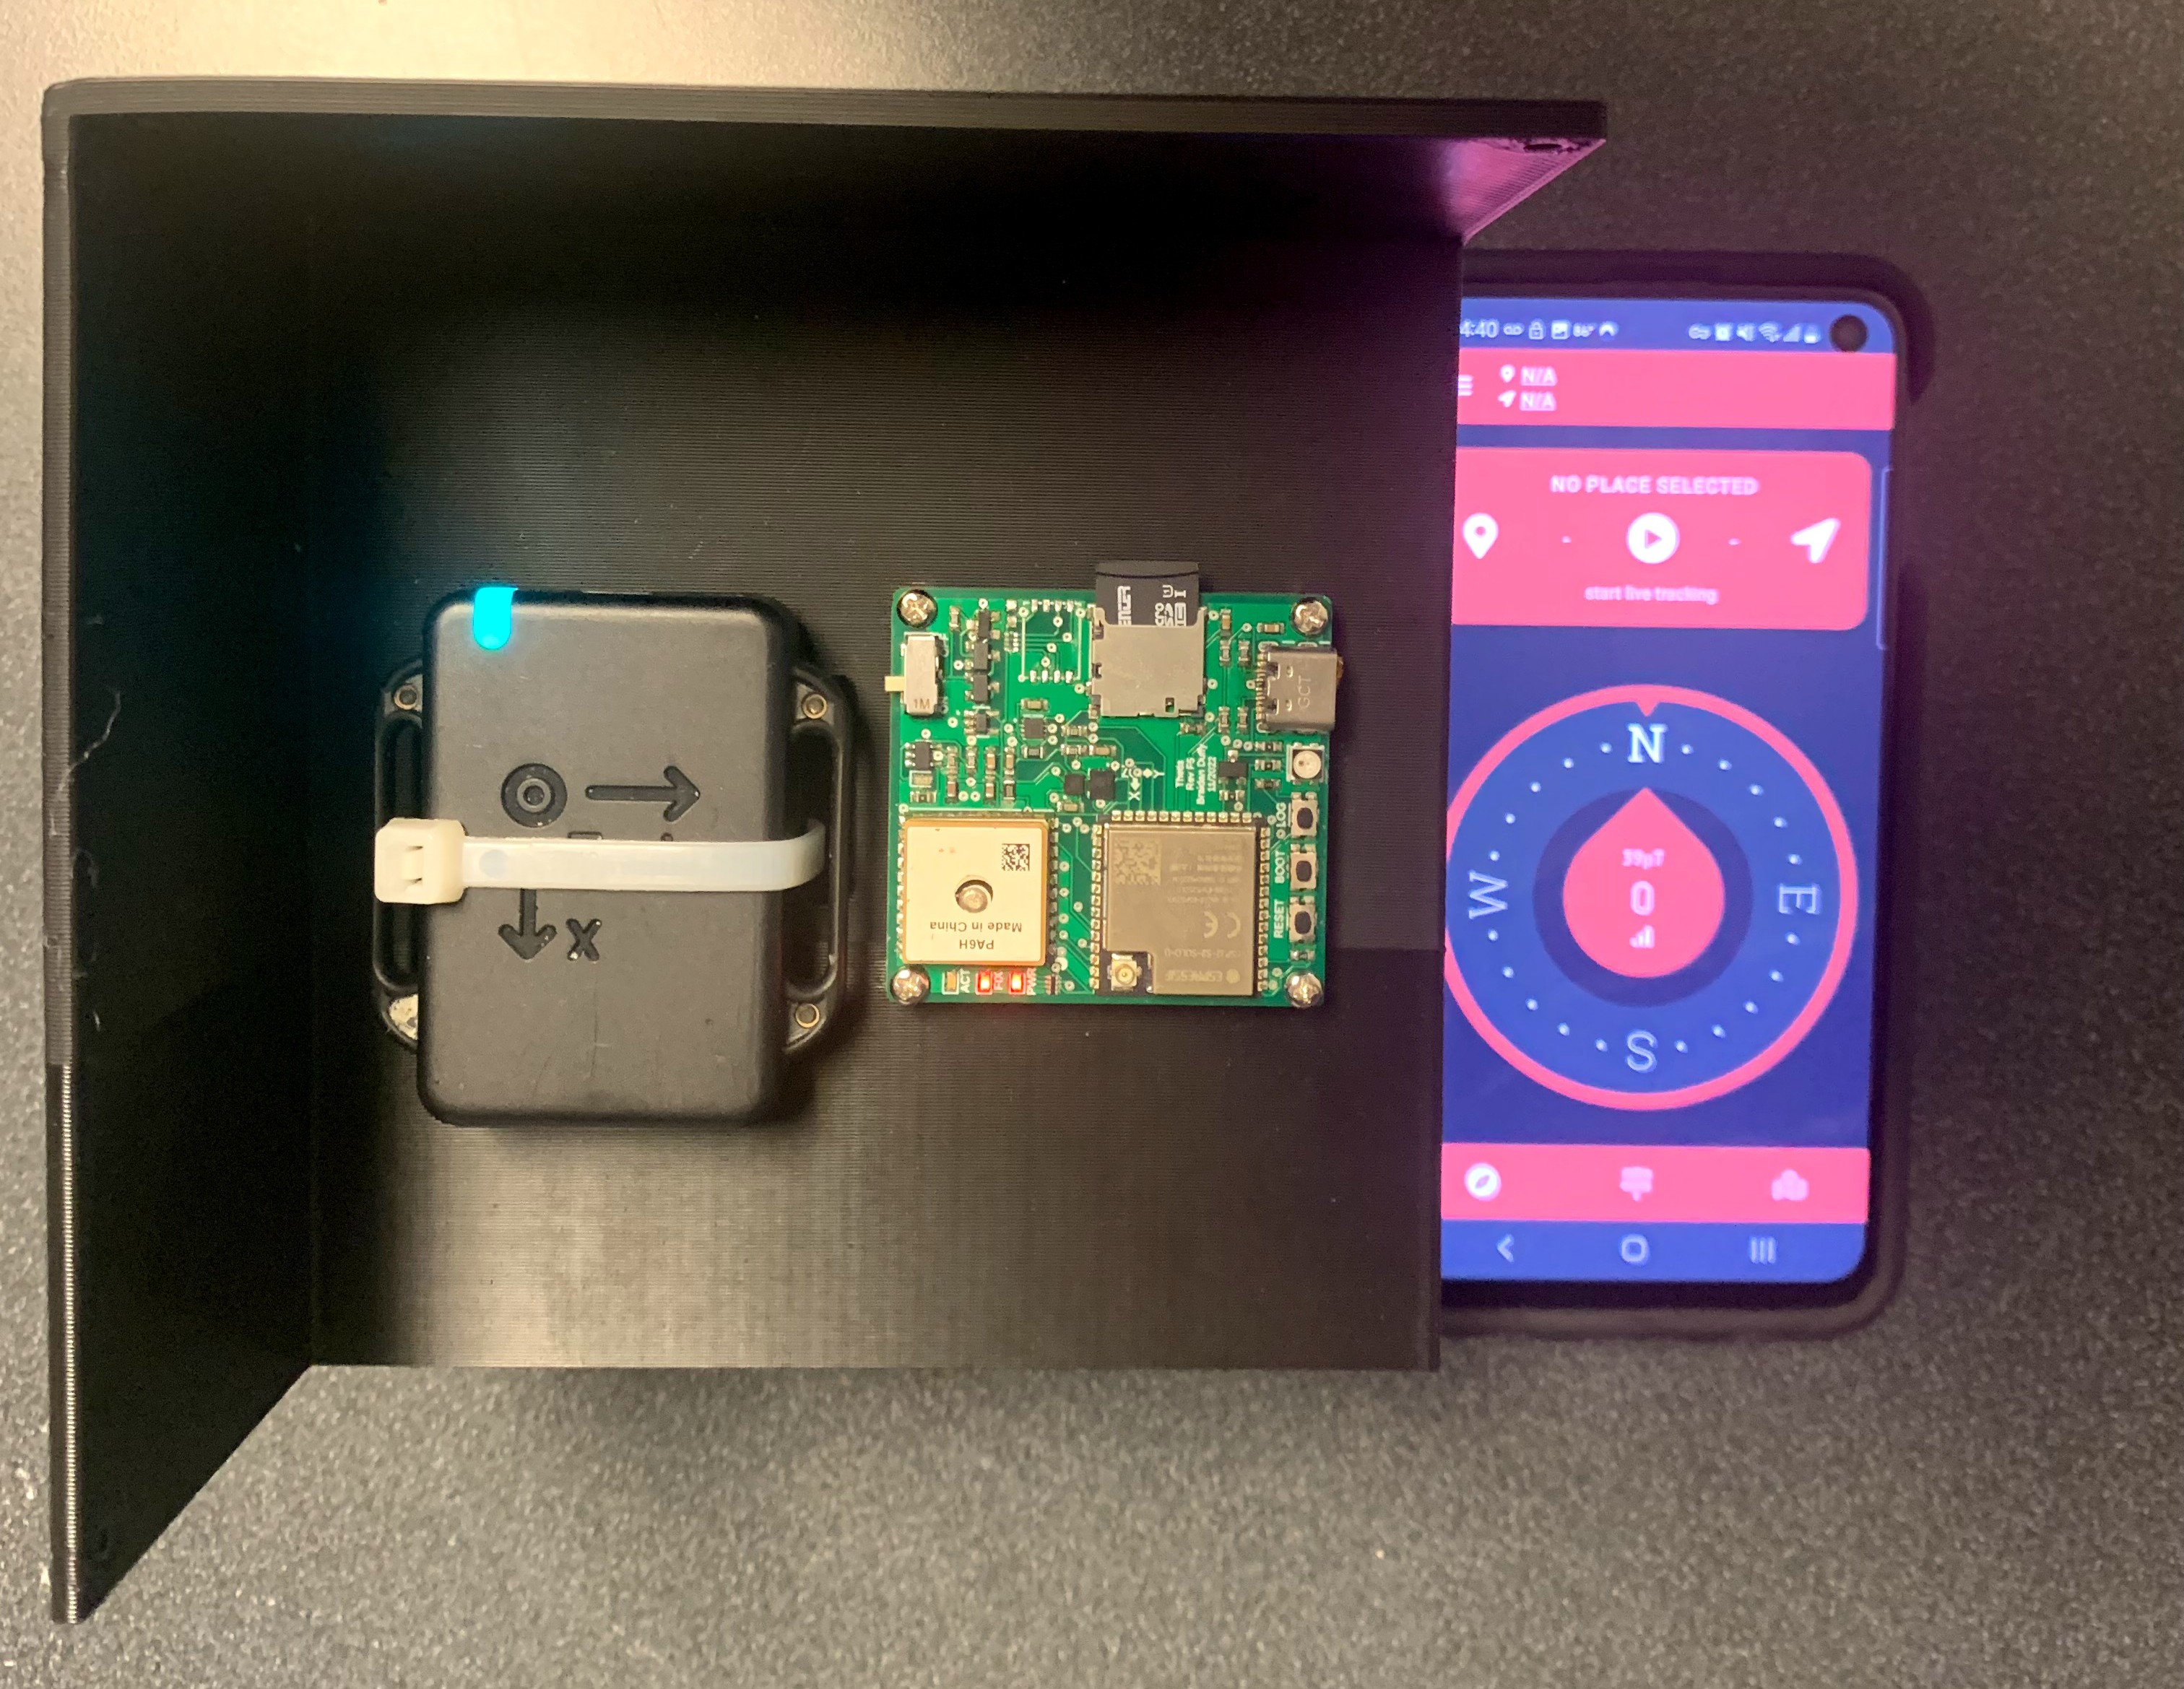
\includegraphics[height=2in]{calibration/calibration_cube_compass.jpg}
    \caption{Calibration cube aligned with an external compass.}
    \labfig{calibration_cube_compass}
\end{figure}

\section{Results} \labsec{calibration_results}
The calibration data was collected and ran through a calibration script in \cite{Thetis-Scripts}.
The raw log files were converted to CSVs using the x-IMU3 software conversion tool\footnote{\url{https://github.com/xioTechnologies/x-IMU3-Software/blob/main/Examples/Python/file_converter.py}}.
The resultant Magnetometer, Inertial, and Quaternion files were imported to the script using the \lstinline[style=customInline]|pandas| library.
Then, they were initially processed into dictionaries the contained the relevant data for each device for each test for each axis.

The raw data from each test dataset was cleaned by removing outliers and then windowed to an approximately 15-second span in the center of the data.
Windowing helped reduce processing time and automatically removed the heads and tails from the Thetis gyroscope plots, making analysis easier.
This cleaned and windowed data were placed back into the dictionary for each dataset and then plotted into the raw data figures shown in Appendix \ref{chap:raw_data_plots}.

After plotting the raw inertial data, the calibration parameters were calculated for the accelerometer and gyroscope.
The process used the mathematical techniques described in Chapter \ref{chap:background} and several external toolboxes.
For determining the misalignment sensitivity matrices, the \lstinline[style=customInline]|scipy.optimize.minimize| toolbox was used with the Sequential Least Squares Programming (SLSQP) method.
For this method, the objective function defined in Equation \ref{eq:misalignment_obj_func} was used as the scalar function.

After producing the inertial calibration parameters, the script calculates the root-mean-square-error between for the devices with respect to ground truth and each other. 
These plots are shown in the following section.
After determining the inertial RMSE, the magnetic parameters are calculated using the previously discussed mathematical methods and several plots are generated.

\subsection{Magnetometer}
This section shows the magnetometer calibration data as it is processed by the calibration script.
Note that the x-IMU3 does not have a hard or soft iron plot as it was already calibrated to remove these distortions.

% \begin{figure}[h!]
%     \centering
%     \begin{subfigure}[b]{0.6\textwidth}
%         \centering
%         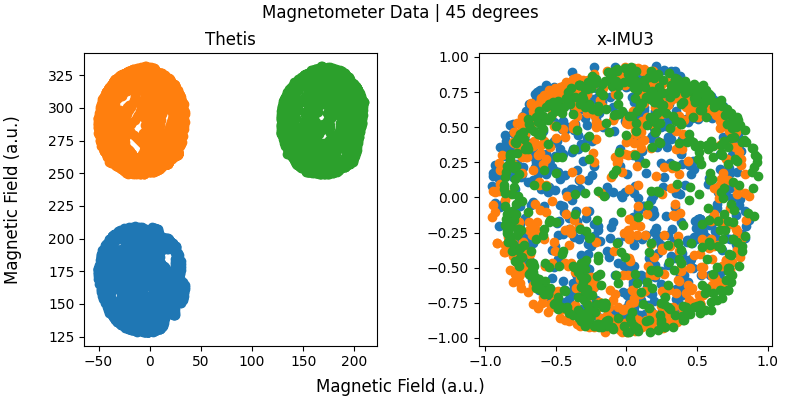
\includegraphics[width=\textwidth]{calibration/raw/raw_mag_all_45.png}
%         \caption[Raw Magnetometer Readings]{Raw magnetometer calibration data from Thetis (left) and the x-IMU3 (right)}
%         \labfig{mag_cal_raw}
%     \end{subfigure}
%     \hfill
%     \begin{subfigure}[b]{0.3\textwidth}
%         \centering
%         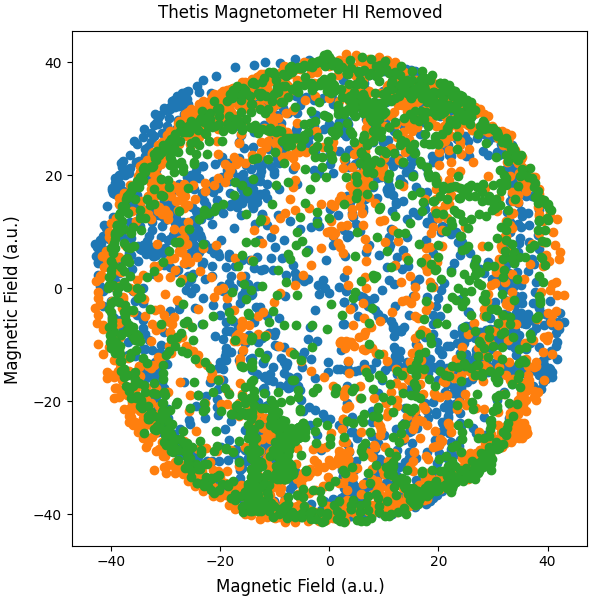
\includegraphics[width=\textwidth]{calibration/prelim/mag_hard_iron_removed.png}
%         \caption[Hard Iron Distortion Removed]{Thetis magnetometer calibration data with hard iron distortion removed.}
%         \labfig{mag_cal_hid_removed}
%     \end{subfigure}
%     \hfill
%     \begin{subfigure}[b]{0.5\textwidth}
%         \centering
%         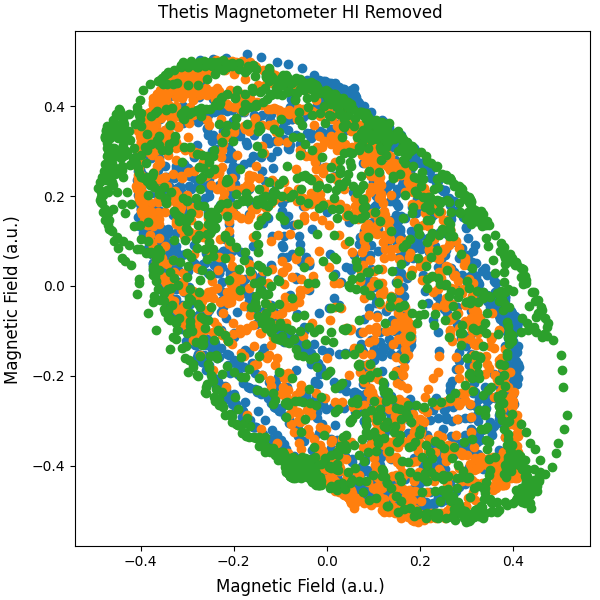
\includegraphics[width=\textwidth]{calibration/prelim/mag_soft_iron_removed.png}
%         \caption[Soft Iron Distortion Removed]{Magnetometer calibration data with soft and hard iron distortion removed.}
%         \labfig{mag_cal_sid_removed}
%     \end{subfigure}
%        \caption{Magnetometer calibration process}
%        \labfig{magnetometer_calibration_process}
% \end{figure}
\begin{figure}[h!]
    \centering
    \subfloat[Raw magnetometer calibration data from Thetis (left) and the x-IMU3 (right)]{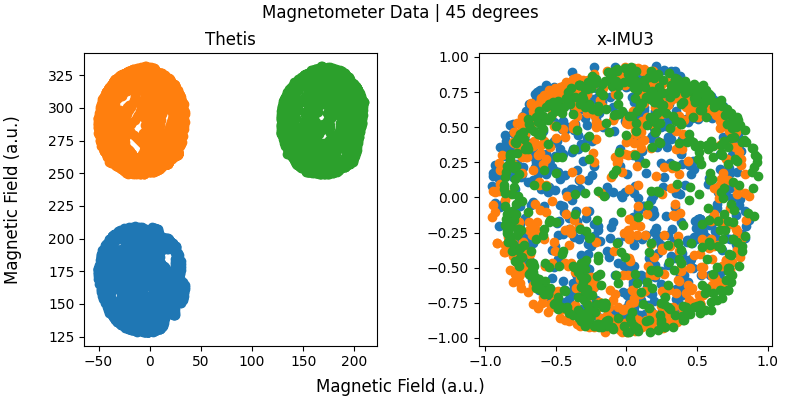
\includegraphics[width=0.6\textwidth]{calibration/raw/raw_mag_all_45.png}\label{subfig:mag_cal_raw}}\hskip3ex
    \subfloat[Thetis magnetometer calibration data with hard iron distortion removed.]{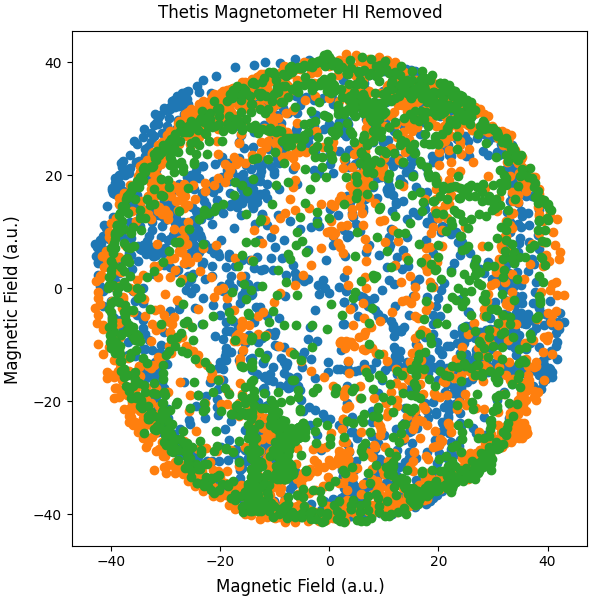
\includegraphics[width=0.4\textwidth]{calibration/prelim/mag_hard_iron_removed.png}\label{subfig:mag_cal_hid_removed}}\hskip3ex
    \subfloat[Magnetometer calibration data with soft and hard iron distortion removed.]{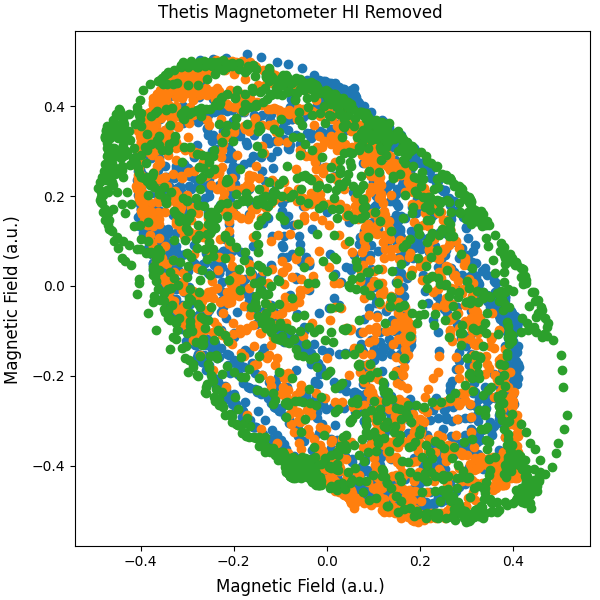
\includegraphics[width=0.4\textwidth]{calibration/prelim/mag_soft_iron_removed.png}\label{subfig:mag_cal_sid_removed}}
	\caption{Magnetometer calibration process}
	\labfig{calibration_tools}
\end{figure}

The calibration data yielded the following parameters:

\begin{align*}
    \pmb{v} &= 
    \begin{bmatrix}
        -8.0752 \\
        168.7446 \\
        290.5438 \\
    \end{bmatrix} \\
    W^{-1} &= 
    \begin{bmatrix}
        0.0072 & -0.0040 & -0.0049 \\
        -0.0040 & 0.0100 & -0.0048 \\
        -0.0049 & -0.0048 & 0.0106 \\
    \end{bmatrix}
\end{align*}

\subsection{Gyroscope}

The calibration data yielded the following parameters:

\begin{align*}
    \pmb{b}_g &= 
    \begin{bmatrix}
        -0.0003 \\
        0.0002 \\
        0.0002 \\
    \end{bmatrix} \\
    S_g &= 
    \begin{bmatrix}
        1.0110 & 0      & 0 \\
        0      & 0.9672 & 0 \\
        0      & 0      & 1.0041 \\
    \end{bmatrix} \\
    M_g &= 
    \begin{bmatrix}
        1       & 0.0037 & 0.0399 \\
        0.0100  & 1      & -0.0075 \\
        -0.0259 & 0.0105 & 1 \\
    \end{bmatrix}
\end{align*}

\begin{figure}[h!]
    \centering
    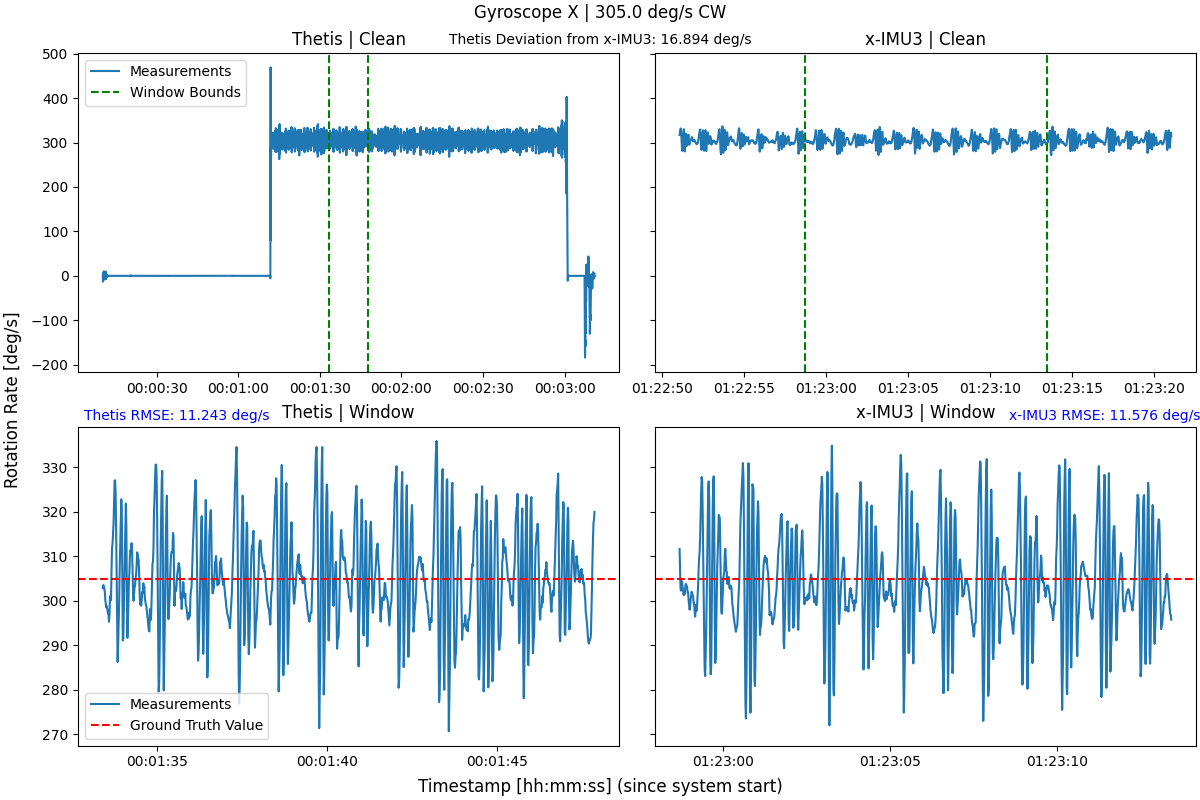
\includegraphics[width=\textwidth]{calibration/raw/raw_gyro_x-axis_305.png}
    \caption[Raw and windowed gyroscope data]{Raw and windowed gyroscope data from Thetis (left) and the x-IMU3 (right).}
    \labfig{raw_gyro_data}
\end{figure}

\begin{figure}[h!]
    \centering
    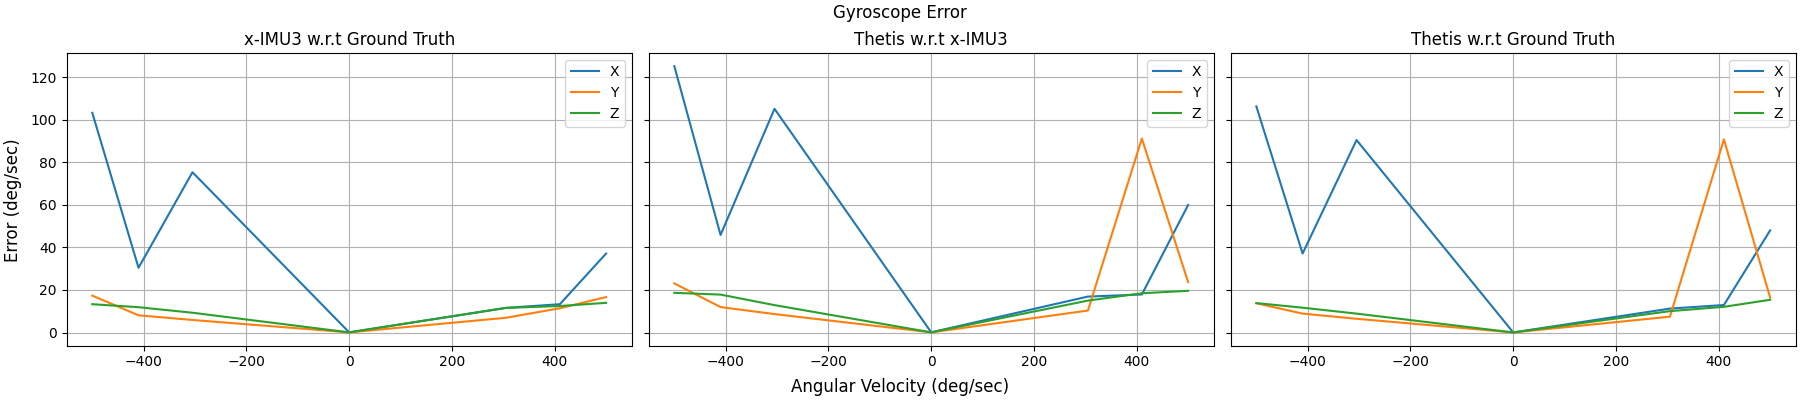
\includegraphics[width=\textwidth]{calibration/prelim/prelim_gyro.png}
    \caption[Cumulative gyroscope error]{Root-Mean-Square-Error during calibration across all axes and test speeds. From left to right, Thetis with respect to the ground truth, Thetis with respect to the x-IMU3, and the x-IMU3 with respect to the ground truth.}
    \labfig{prelim_gyro_data}
\end{figure}

\newpage 
\subsection{Accelerometer}

\begin{figure}
    \centering
    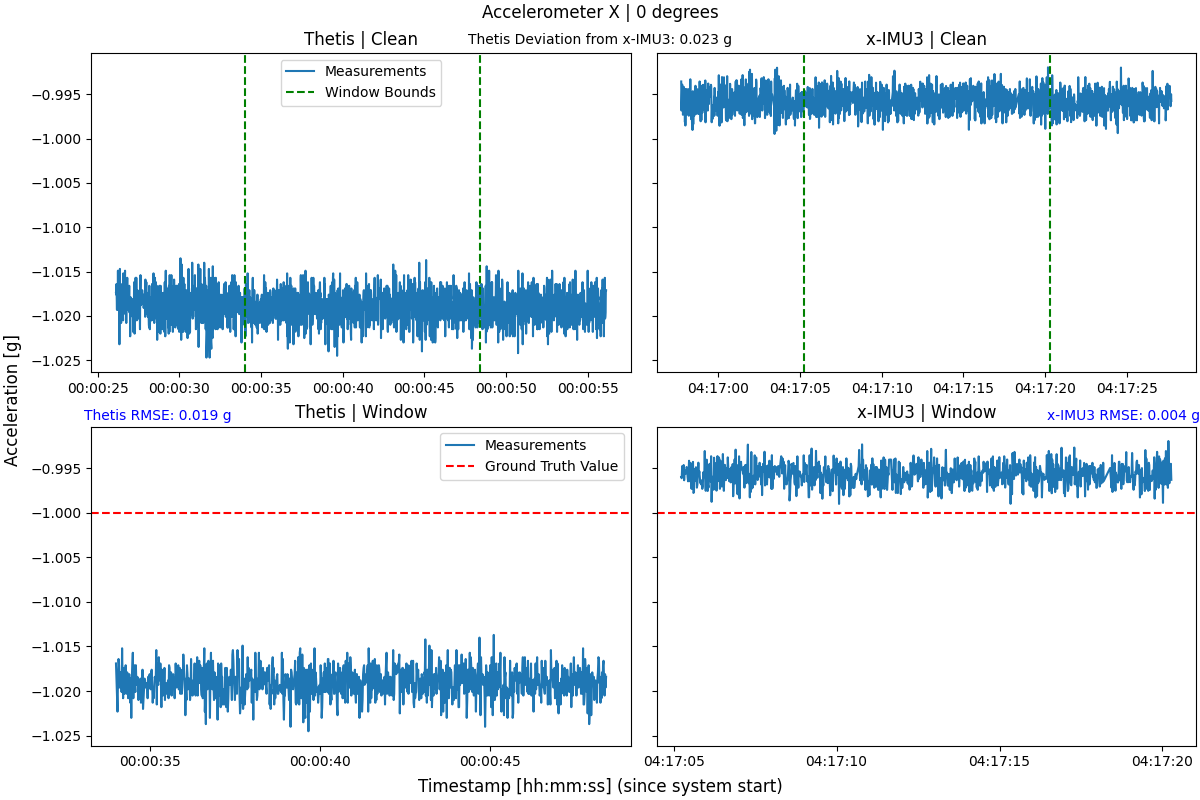
\includegraphics[width=\textwidth]{calibration/raw/raw_accel_x-axis_0.png}
    \caption[Raw and windowed accelerometer data]{Raw and windowed accelerometer data from Thetis (left) and the x-IMU3 (right).}
    \labfig{raw_accel_data}
\end{figure}

\begin{figure}
    \centering
    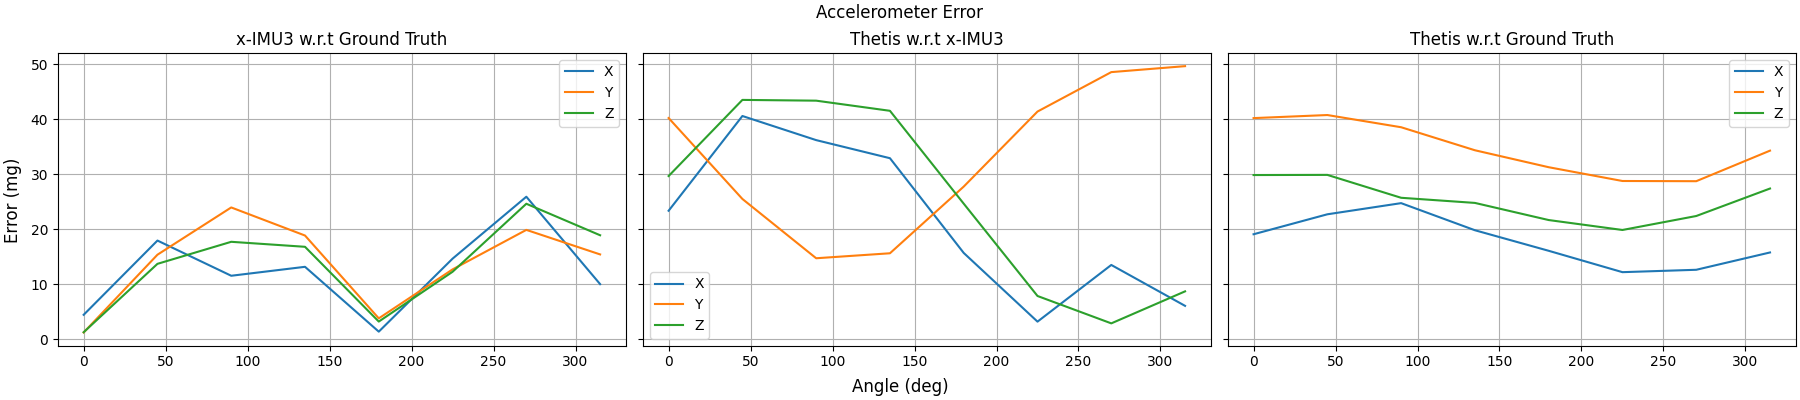
\includegraphics[width=\textwidth]{calibration/prelim/prelim_accel.png}
    \caption[Cumulative accelerometer error]{Root-Mean-Square-Error during calibration across all axes and test orientations. From left to right, Thetis with respect to the ground truth, Thetis with respect to the x-IMU3, and the x-IMU3 with respect to the ground truth.}
    \labfig{prelim_accel_data}
\end{figure}

The calibration data yielded the following data:

\begin{align*}
    \pmb{b}_a &= 
    \begin{bmatrix}
        -0.0243 \\
        0.0342 \\
        0.0112 \\
    \end{bmatrix} \\
    S_a &= 
    \begin{bmatrix}
        0.0171 & 0      & 0 \\
        0      & 0.6617 & 0 \\
        0      & 0      & 1.0022 \\
    \end{bmatrix} \\
    M_a &= 
    \begin{bmatrix}
        1        & 0.0033 & 0.0401 \\
        -0.3294  & 1      & -0.0067 \\
        -58.2018 & 0.0135 & 1 \\
    \end{bmatrix}
\end{align*}

\section{Discussion}
From the calibration results, we can identify several potential errors in the employed analytical methods.

\paragraph*{Magnetometer} First, regarding Figure \ref{subfig:mag_cal_sid_removed}, the shape of the data points changes from spherical to ellipsoidal with a higher eccentricity than expected.
The measurements also decrease in intensity by two orders of magnitude. 
This indicates that 1) the Li ellipsoid fitting algorithm may not be applied using the correct radius for the target ellipsoid, and 2) that the target ellipsoid has too high of eccentricity to be fitted into a sphere.
Identifying and implementing a fix to this issue is currently out of the scope of this thesis.
Therefore, it is recommended that only the hard iron offset, $\pmb{v}$, be used for calibrating magnetic measurements for now.

With the hard iron offset applied to the data, the following RMSE values and per cent errors are reported in Table \ref{tab:magnetometer_errors}.
Here, we can see a larger deviation from Thetis with respect to the ground truth and the x-IMU3, but the couple of percentage points difference between Thetis and the x-IMU3 could be caused by sensor performance and the x-IMU3's application of soft iron distortion compensation.

\begin{table}[h!]
    \renewcommand{\arraystretch}{1.75}
    \centering
    \begin{tabular}{| m{5cm} | c | c |}
        \hline
        \textbf{Comparison} & \textbf{RMSE (uT)} & \textbf{Percent Error} \\
        \hline
        Thetis w.r.t Ground Truth\tablefootnote{As measured curing calibration, the magnitude of the magnetic field was ~45 uT} & 3.49 & 7.33\% \\
        Thetis w.r.t x-IMU3\tablefootnote{From the x-IMU3 data sheet, the x-IMU3 readings were converted from a.u. to uT using 50 uT/a.u. as stated in the calibration certificate} & 4.92 & 9.34\% \\
        x-IMU3 w.r.t Ground Truth\footnotemark[\value{footnote}] & 2.48 & 4.69\% \\
        \hline
    \end{tabular}
    \caption{Comparison errors between the magnetometers onboard Thetis and the x-IMU3}
    \labtab{magnetometer_errors}
\end{table}

\paragraph*{Gyroscope} In the gyroscope calibration data, we can see a lot of error introduced via noise into the measurements.
The calibration machine does not spin at a constant rate and seems to have an induced oscillation and variance as the plate rotates.
Additionally, the calibration cube's moment of inertia is not centered directly on the rotation axes because the object is not weighted symmetrically.
These errors lead to the large RMSE values shown in Figure \ref{fig:prelim_gyro_data} between Thetis and the x-IMU3.
The large noise magnitudes for some of the x- and y-axis tests also introduced exceedingly large errors for the calibration data upwards of 100 deg/sec (approximately 20\%).

The errors are consistent across the Thetis and x-IMU3 datasets suggesting that they are systematic errors with the calibration machine, and not related to any sensor itself.
When the machine works properly (i.e. minimal noise in the data set), the error in Thetis and x-IMU3 with respect to each other and the ground truth varies between 5\% and 10\% which is within reason, given that Thetis is uncalibrated and not accounting for any measurement errors itself.
If the machine was more stable and able to give more useful data, the calibration parameters could be calculated better and applied to reduce Thetis's measurement error.
However, because of the large discrepancies in the calibration data and error, it is not recommended to use the calculated calibration parameters for the gyroscope.

\paragraph*{Accelerometer} The accelerometer calibration data looks good at first glance except for the average error being several tenths of a g.
Even on the x-IMU3, the error remains higher than provided in the calibration certificate, implying that there are errors in the test apparatus.
Most likely, the gear and socket were not perfectly flat and aligned with the gravitational field.
Therefore, the other axes sensed the gravitational field more and caused the readings on the sensing axis to skew.
The error persisted throughout all angles of testing on all axes as shown in Figure \ref{fig:prelim_accel_data}, further reinforcing the theory that it was introduced by the testing apparatus rather than the instruments themselves.

A very concerning problem are the misalignment sensitivity matrices calculated from the calibration data.
The sensitivity matrix, $S_a$, should have values around 1 in the diagonal.
The x-IMU3 calibration certificate shows that the sensitivity values for that device are within 1\% of unity.
The calculated values in $S_{a,11}$ and $S_{a,22}$ are significantly less than 1, meaning that the measurements will not be near their true value.
Additionally, the misalignment matrix should have values that are near zero surrounding the diagonal 1's.
The value of $M_{a,31}$ is $-58.2018$ which strongly indicates this calibration was not successful.

The most likely reason these discrepancies have occurred is because of the method from which the sensitivity and misalignment matrices are calculated.
They are calculated using a non-linear optimization algorithm that tries to minimize the error found in an objective function (Equation \ref{eq:misalignment_obj_func}).
As the minimization occurs, it can fall into local minima that fulfill the boundary conditions laid out for this methodology, but will result in invalid calibration parameters.
Further research needs to be performed on the best optimization techniques to find these calibration parameters.
This research is out of the scope of this thesis due to the technical involvement.
Based on these errors, it is not recommended to use the accelerometer calibration parameters calculated here.

\paragraph*{Conclusion} Due to errors in the inertial data collection and analytical methods, Thetis cannot have its accelerometer or gyroscope calibrated at this time.
However, the magnetometer can be calibrated using only the hard iron offset.
The calibration data taken between Thetis and the x-IMU3 suggests that the devices perform closely with one another and that given more time and expertise with calibration, Thetis can become reasonably equivalent to the x-IMU3 in terms of sensor performance under the methodologies described above.
The data collection process also demonstrated that Thetis can collect measurements reliably via its on board micro SD card storage and that can be offloaded and processed.
The data was collected at 64 Hz sample rate which also validated some system requirements - this will be further explained in the next chapter.
%%-----------------Chapter 5---------------------------
\chapter{Verification and Validation} \labchap{verification_validation}
Now that we have an instrument designed, how can we determine if it meets requirements or not?
The system can be verified and then validated using a variety of techniques.
First, to verify that a requirement is present, the component or subsystem can be examined independently.
If it passes examination, we can update the traceability matrix to reflect that the requirement is now verified.
Once the feature is integrated with the entire system, then we can determine if it is validated or not.
Instead of examining the feature independently, it will be done so with the entire system to ensure that it functions properly.
These examinations can fall under four main types:

{
\renewcommand{\descriptionlabel}[1]{\hspace{\labelsep}\textbf{#1}}
\begin{description}
    \item[Inspection:] The nondestructive examination of a product or system using one or more of the five senses (visual, auditory, olfactory, tactile, taste). 
    It may also include simple physical manipulation and measurements.
    
    \item[Demonstration:] The manipulation of the product or system as it is intended to be used to verify that the results are as planned or expected.								
    
    \item[Test:] The verification of a product or system using a controlled and predefined series of inputs, data, or stimuli to ensure that the product or system will produce a very specific and predefined output as specified by the requirements.								
    
    \item[Analysis:] The verification of a product or system using models, calculations and testing equipment.
    Analysis allows someone to make predictive statements about the typical performance of a product or system based on the confirmed test results of a sample set or by combining the outcome of individual tests to conclude something new about the product or system.
    It is often used to predict the breaking point or failure of a product or system by using nondestructive tests to extrapolate the failure point.
\end{description}
}

For the following chapter, we shall examine each of Thetis' design capabilities from Tables \ref{tab:threshold_capabilities} through \ref{tab:stretch_capabilities} and verify their presence on the latest design.
Then, we shall do the same for the stakeholder requirements.

\section{Threshold Capabilities} \labsec{threshold_capabilities}

\newcommand{\yes}{\cellcolor[HTML]{63BE7B}Y}
\newcommand{\no}{\cellcolor[HTML]{F8696B}N}  %{0.9}

{\fontsize{8pt}{8pt}\selectfont
\begin{table}[ht!]
    \centering
	\renewcommand{\arraystretch}{1.5} % Set row height
	\begin{tabular}{| c | m{0.55\textwidth} | c | c | c |}
		\hline
		\multicolumn{5}{| c |}{\textbf{Threshold}} \\
		\hline
		\textbf{ID} & \multicolumn{1}{c|}{\textbf{Description}} & \textbf{Verified?} & \textbf{Validated?} & \textbf{Status} \\
		\hline
		101 & The system must be housed in an IP67-rated enclosure & \yes & \yes & D \\
		102 & The system enclosure must fit within the volume of 8" x 5" x 1.25" & \yes & \yes & D \\
		103 & The system software and firmware will be fully open-source & \yes & \yes & D \\
		104 & The system shall record inertial measurements at a minimum frequency of 64 Hz & \yes & \yes & D \\
		105 & The system shall be able to store data locally for up to 4 hours continuously & \yes & \no & TIP \\
		106 & The system shall be able to be operate for up to 4 hours continuously & \yes & \no & A \\
		107 & The system shall have simple human interface mechanism for status and logging & \yes & \yes & D \\
		108 & The system firmware shall be an open-architecture & \yes & \yes & A \\
		109 & The system will be fully documented & \no & \no & A \\
		110 & The system shall use version control software to track changes & \yes & \yes & D \\
		111 & The operator shall be able to offload data from the system & \yes & \yes & D \\
		112 & The system shall be capable of being assembled by hand using basic soldering tools & \yes & \yes & D \\
		\hline
	\end{tabular}
	\caption{Verification and validation of threshold capabilities}
	\labtab{vv_threshold_capabilities}
\end{table}
}

\paragraph*{101 - The system must be housed in an IP67-rated enclosure} This capability was initially verified by locating a suitable enclosure for Thetis and confirming with the manufacturer through the product data sheet that the system was properly rated.
Then, it was validated by placing the enclosure onto a Remotely Operated Vehicle (ROV) and descending down to 20-feet of depth while the ROV performed a mission.
Paper towels were placed within the enclosure so that if any water breached the seals, it would be immediately apparent.
This represented a worst-case scenario and the enclosure held its seal meaning that it exceeded the capability requirement.

\begin{figure}[h!]
    \caption[ROV Setup]{Thetis (bottom) attached to a Blue ROV2 frame for enclosure testing.}
    \labfig{thetis_rov}
    \centering
    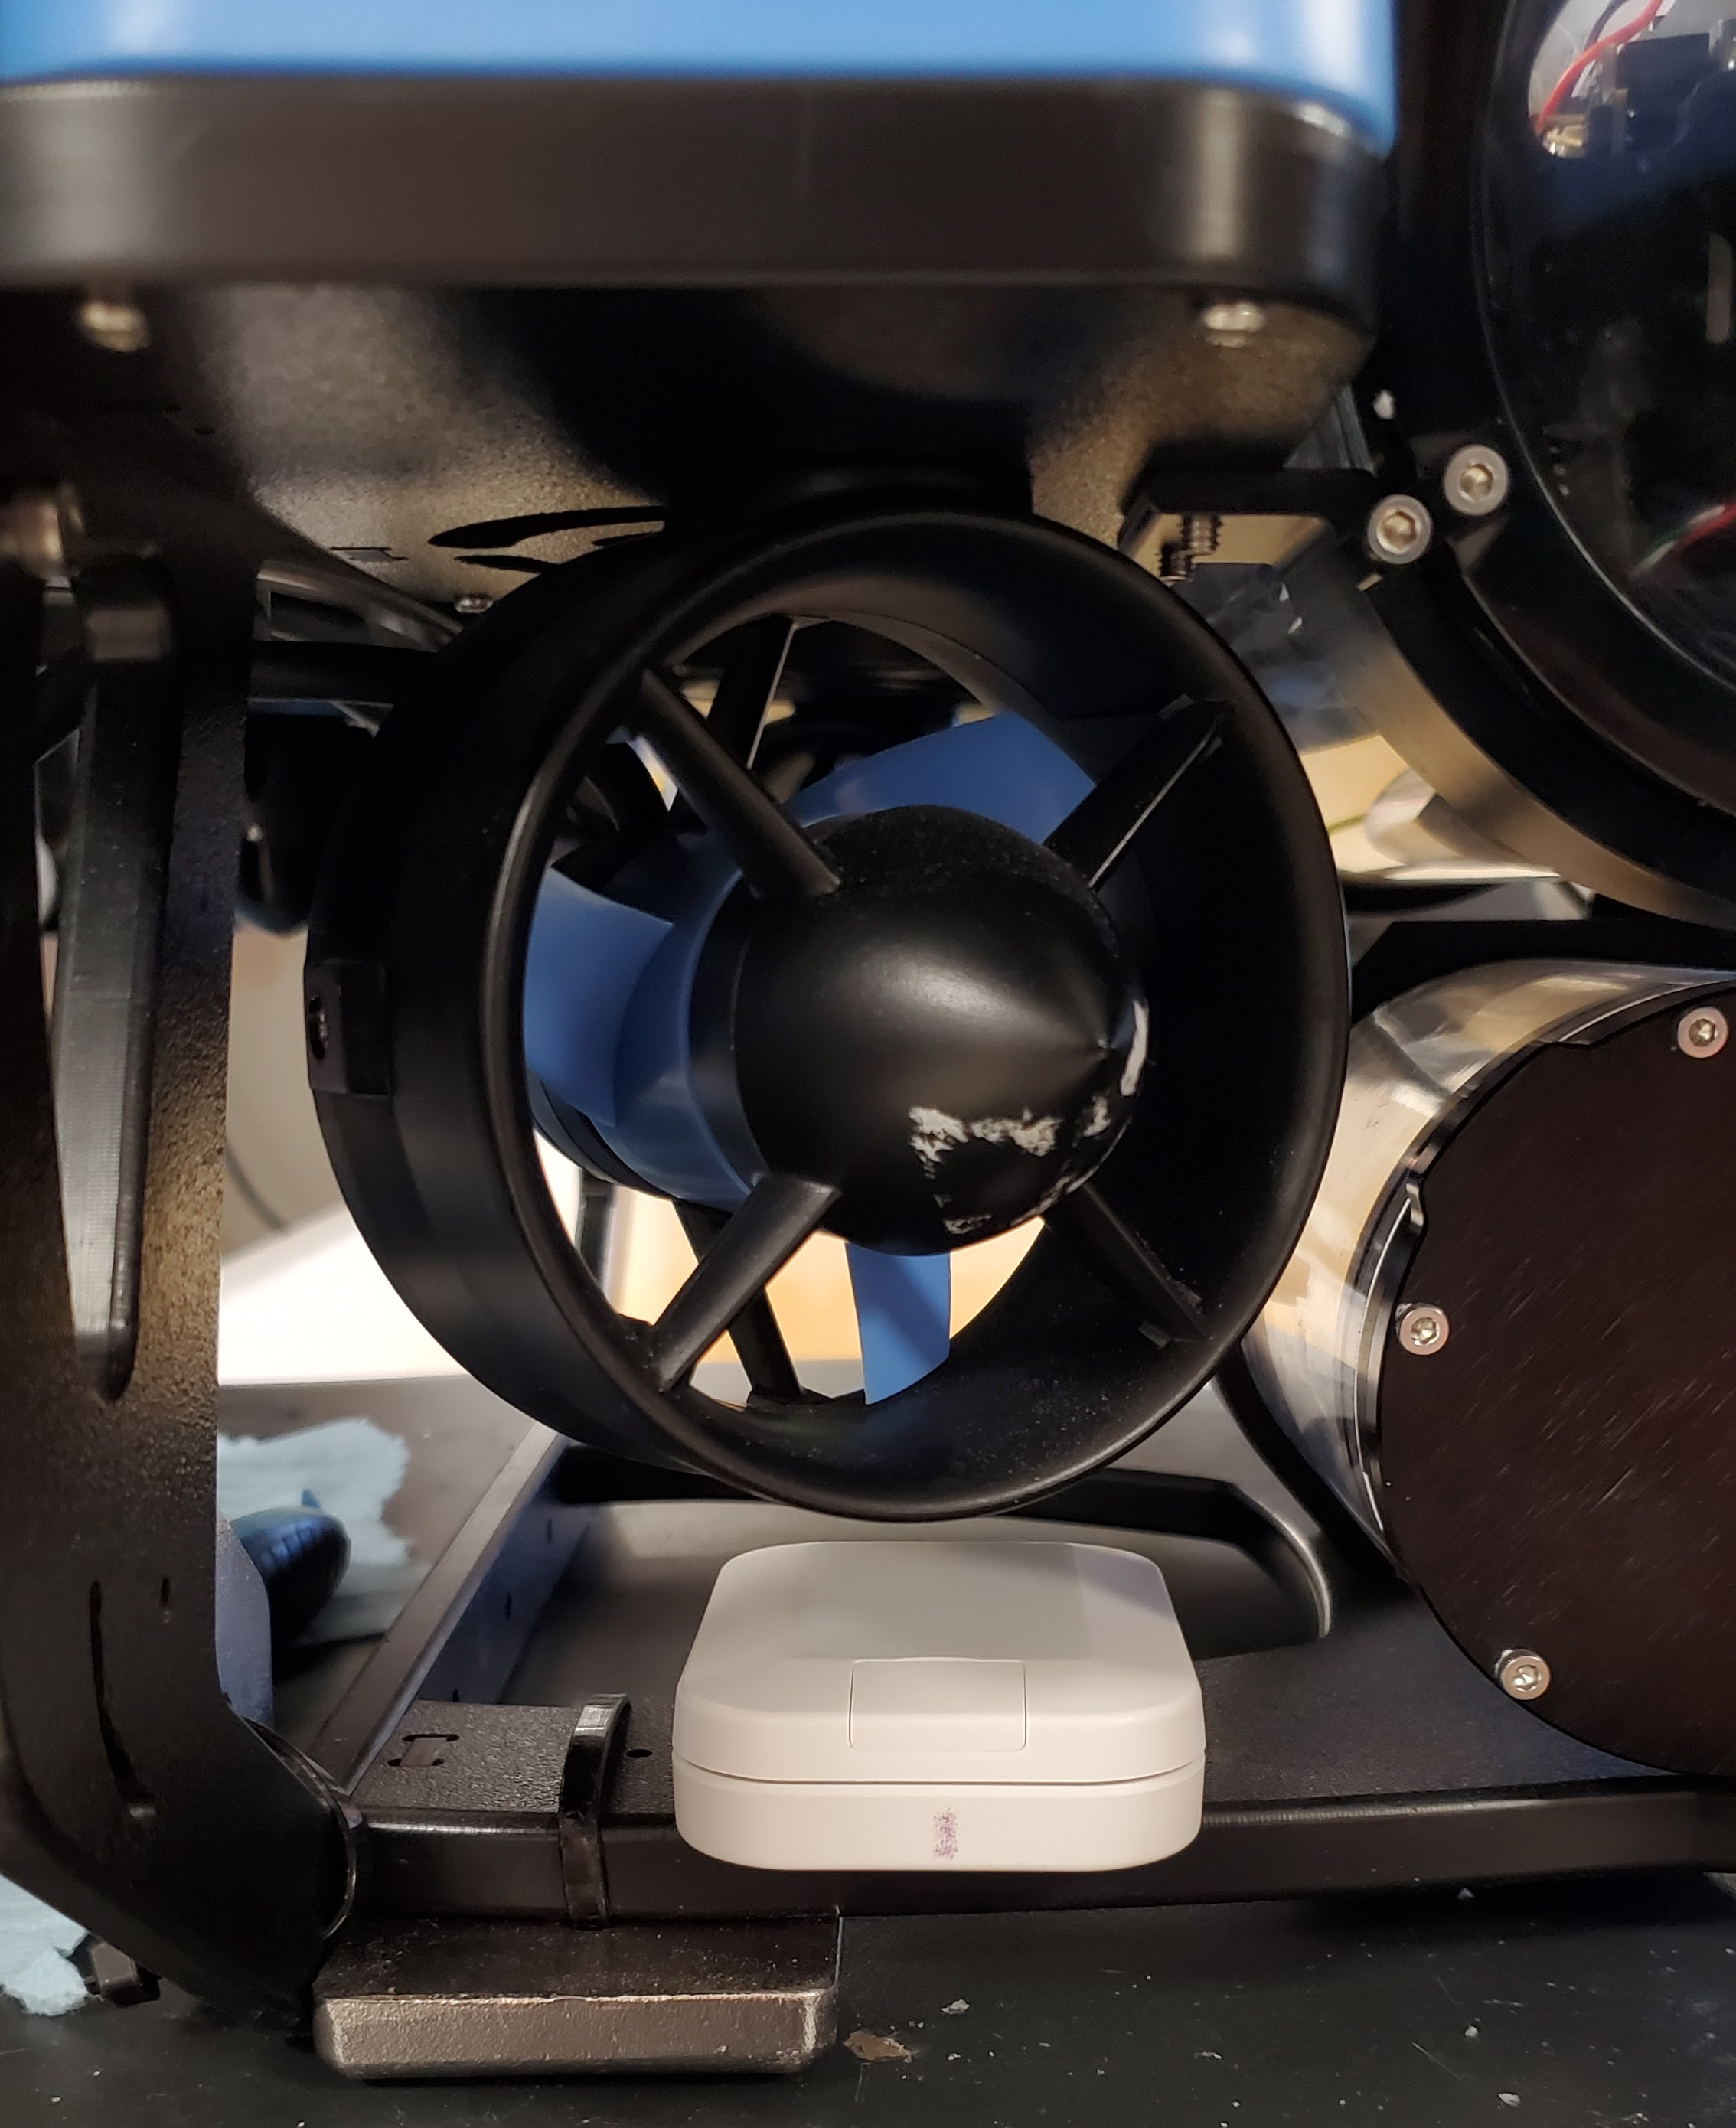
\includegraphics[height=2.5in]{verify_validate/thetis_rov.jpg}
\end{figure}

To represent a more realistic use case, Thetis was placed into a cutout on a surfboard and deployed into the ocean to catch some waves.
Out nine separate deployments, the case seal failed three different times:

\begin{enumerate}
    \item A screw was not present in one corner, thereby not clamping that section of the sealing material, 
    \item a screw was over-torqued and caused the area around the screw to crack, bypassing the seal, and 
    \item the same case as before was used accidentally.
\end{enumerate}

All three failures were due to operator error proving that careful procedures need to be implemented for actual deployments.
However, when the case was properly sealed by operators, the seals held and the electronics within were not damaged, even when completely submerged and subjected to dynamic forces as the surfboard rolled and slammed into waves.

\begin{figure}[h!]
    \caption[Surfboard Setup]{Thetis (right) and the x-IMU3 (left) secured in a cutout on a modified surfboard during a deployment.}
    \labfig{thetis_surfboard}
    \centering
    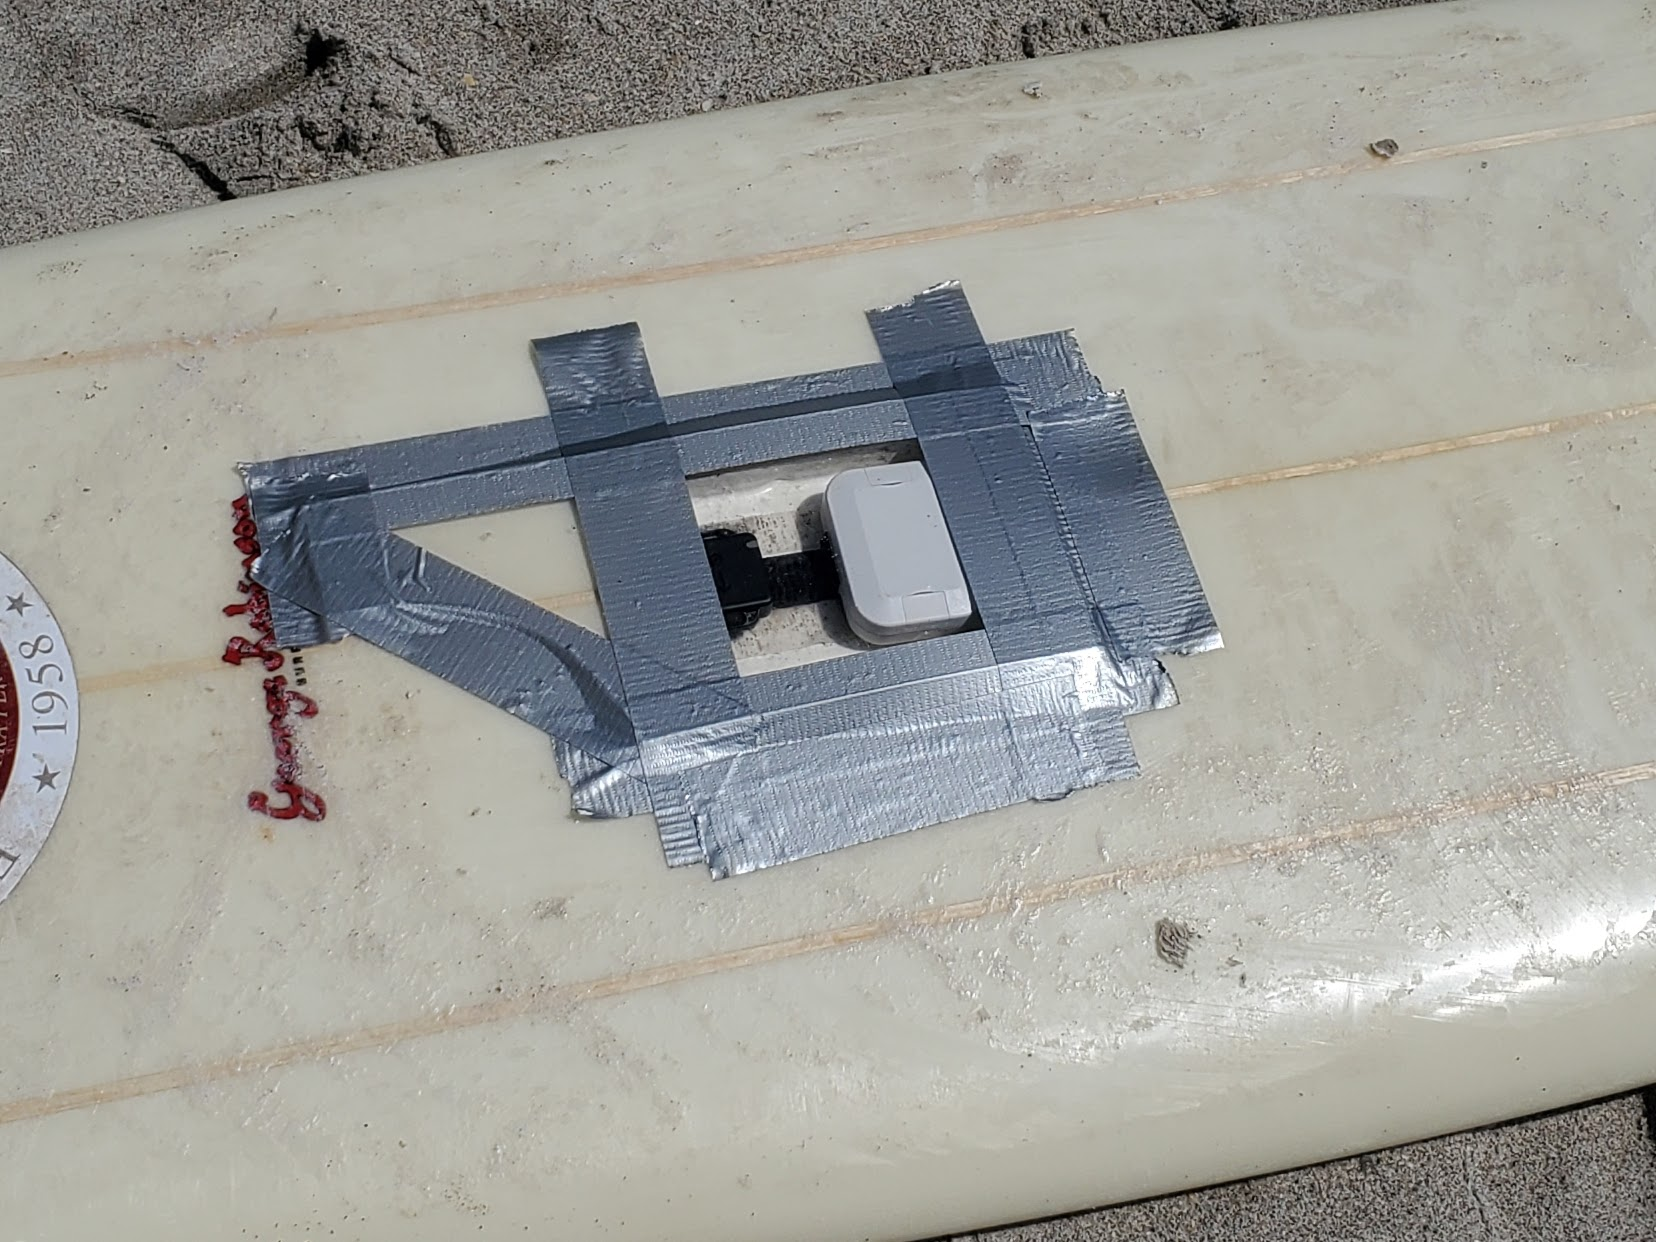
\includegraphics[height=2.5in]{verify_validate/thetis_surfboard.jpg}
\end{figure}

\paragraph*{102 - The system enclosure must fit within a volume of 8" x 5" x 1.25"} Like Capability 101, this was initially verified by inspection during the search for this enclosure and confirming the enclosure dimensions with the manufacturer.
Then, it was validated by placing it securely into the cutouts in the surfboard made for the iPhone 6S - the device Thetis is intended to replace, as shown in Figure \ref{fig:thetis_surfboard}.

\paragraph*{103 - The system software and firmware will be fully open-source} This capability is both verified and validated by inspection as the code is readily accessible on GitHub.
The firmware is broken into several sub repositories: \href{https://github.com/Legohead259/Thetis-Firmware}{Thetis-Firmware}, \href{https://github.com/Legohead259/ThetisLib}{ThetisLib}, \href{https://github.com/Legohead259/xioAPI-Arduino}{xioAPI-Arduino}, \href{https://github.com/Legohead259/Timer-Events-Arduino}{Timer-Events-Arduino}, and \href{https://github.com/Legohead259/Fusion-Arduino}{Fusion-Arduino} all of which are under the MIT license and available.
Thetis has several tangential software packages that are also open source such as the \href{https://github.com/Legohead259/Thetis-Scripts}{scripts repository} used for data processing and analysis, the \href{https://github.com/xioTechnologies/x-IMU3-Software}{x-IMU3 GUI} used to visualize data and log from a host computer, and the \href{https://github.com/Legohead259/Thetis-Calibration}{code for the calibration machine}.

\paragraph*{104 - The system shall record inertial measurements at a minimum frequency of 64 Hz} This capability requires a demonstration in order to be verified and validated.
We can initially inspect the firmware to ensure that the inertial measurements are taken every 15.6 milliseconds, but it is not guaranteed that the system can consistently take measurements at that speed.
Therefore, the best way to demonstrate this capability was during the calibration procedure detailed in Section \ref{sec:calibration_methodologies}.
Thetis was set to record at 64 Hz and when the data was offloaded, it was confirmed to be taken at the appropriate interval.
Therefore, this capability has been verified and validated within the system.

\paragraph*{105 - The system shall be able to data locally for up to 4 hours continuously} We can analyze the size of logging messages and SD card to determine if this capability is verified.
In the latest version of the firmware, five messages are published to the data storage device: position, inertial, magnetic, quaternion, and euler angle.
Combined, these messages take 198 bytes of space and occur, on average, 64 times per second for 12,672 bytes per second.
There are 14,400 seconds in 4 hours, so multiplying these values together, we get 182.5 megabytes of storage required for 4 hours of use.
The microSD cards used throughout testing are at least 4 gigabytes which gives an estimated 88 hours of continuous logging.
This requirement was validated by running Thetis for four hours continuously and verifying that the log file was successfully created and maintained for that period.

\begin{equation} \labeq{storage_time}
    t_{\text{samples}} = \frac{N_{\text{storage}} [\text{Bytes}]}{198 [\text{Bytes}] \times 64 [\text{s}^{-1}] \times 3600 \left[\frac{\text{s}}{\text{h}}\right]} = \frac{4 [\text{GB}]}{198 [\text{Bytes}] \times 64 [\text{s}^{-1}] \times 3600 \left[\frac{\text{s}}{\text{h}}\right]} = ~88 [\text{h}]
\end{equation}

\paragraph*{106 - The system shall be able to operate for up to 4 hours continuously} For this capability, we can verify it by analysis like the previous one.
We need to start with a couple of assumptions:

\begin{enumerate}
    \item Battery capacity is 420 mAh with 3.7V nominal voltage,
    \item Current consumption without WiFi enabled is ~50 mA, and
    \item Current consumption with WiFi enabled is ~120 mA while transmitting
\end{enumerate}

The latter two assumptions are based on a zeroth-order estimate by summing together the estimated current consumption of the various components as listed in their data sheets.
We can then make a zeroth-order estimate using Equation \ref{eq:battery_life}.
This yields an estimated continuous battery life of 9.4 hours without WiFi and 3.9 hours with WiFi.
An important note about the WiFi estimate is the assumption that it is constantly transmitting.
In reality, this may not be accurate so the battery life may be longer.
If it is below the four-hour threshold, then certain mitigations can be implemented like a burst-mode transmission of data every couple of second or minutes.

\begin{equation} \labeq{battery_life}
    t_{\text{battery}} = \frac{3.7 [\text{v}] \times 420 [\text{mAh}]}{3.3 [\text{V}] \times I_{\text{mode}} [\text{mA}]}
\end{equation}

This capability was validated by running Thetis for four hours continuously from full battery power and ensuring that the battery voltage at the end of the test was within the safe operating limits.
Specific power consumption tests were not performed due to the technical complexity of precisely measuring current draw.

\paragraph*{107 - The system shall have a simple human interface mechanism for status and logging} This is another capability that is straight forward to verify and validate using inspection techniques.
First, to enable logging, an operator only needs to hold the ``log'' button for a half second and the same to stop logging.
To convey status, the RGB LED on-board changes color and pattern.
By referencing the current RGB LED color and pattern with the diagnostic LED table, then the operator can know what the system is doing.
These features were used extensively throughout testing with great success.

\paragraph*{108 - The firmware shall be open architecture} This capability is challenging to fully define and implement, hence its relatively low priority in the threshold category.
To verify this capability has been met, we should consider the difficulty of adding a new feature or component to the firmware.
The firmware uses an object-oriented approach with a star topology.
This means that a new feature can be added by putting it into the appropriate class and tying it to other classes/functions through the main \lstinline[style=customInline]|Thetis| object.
Similarly, we can add a new component by creating a new class in the library and then implementing it in the main class.

Validating this capability will require more research out the scope of this thesis to ensure a proper software architecture is implemented and followed.

\paragraph*{109 - The system will be fully documented} This is another capability that is easy to validate and verify through testing.
Multiple groups of students and stakeholders will be asked to perform simple tasks using Thetis such as replacing a component, assembling the board, adding a firmware feature, or performing calibration.
If the participants are able to perform the task using the available documentation, then this capability has been verified and validated.
Otherwise, the documentation needs to created or modified accordingly.

\paragraph*{110 - The system shall use version control software to track changes} As discussed in Section \ref{ssec:version_control}, GitHub is a centralized VCS solution that enables version history and tracking.
Since all of the software and firmware for Thetis is on GitHub, this capability has been thoroughly verified and validated.
Similarly, all of the hardware was designed in Fusion 360 which implements its own VCS solution and then backed up to GitHub.

\paragraph*{111 - The operator shall be able to offload data from the system} Since the operator needs to be able to pull data off the system after an experiment, this capability is easily verified and validated via demonstration.
During the calibration procedure, data was routinely written to the onboard microSD card and then the operator could pull the card out, load it into a host computer, then transfer the data into an analysis script.
Additionally, data was able to be recorded in real-time through the x-IMU3 GUI application on a host computer through a USB connection to Thetis.
Both of these methods and verified that the capability was implemented and the fact that it could be reliably used throughout multiple tests validated it.

\paragraph*{112 - The system shall be capable of being assembled using basic soldering tools} This capability was clearly demonstrated in Section \ref{ssec:assembly_techniques} where the board is shown to be assembled using solder paste, tweezers, a soldering iron, and hot air.
We can also verify this capability by inspecting the various component used throughout the design.
The smallest component is an `0603' which is 60 thousandths of an inch long by 30 thousandths wide.
While certainly small, they can be manipulated by a steady hand and placed on the board with reasonable accuracy.
For these reasons, this capability has been verified and validated.

\section{Reach Capabilities}

{\fontsize{8pt}{8pt}\selectfont
\begin{table}[ht!]
    \centering
	\renewcommand{\arraystretch}{1.5} % Set row height
	\begin{tabular}{| c | m{0.55\textwidth} | c | c | c |}
		\hline
		\multicolumn{5}{| c |}{\textbf{Reach}} \\
		\hline
		\textbf{ID} & \multicolumn{1}{c|}{\textbf{Description}} & \textbf{Verified?} & \textbf{Validated?} & \textbf{Status} \\
		\hline
		201 & The system shall use a GPS with a minimum 1 Hz update rate for position tracking & \yes & \no & TIP \\
		202 & The system will have a simple logging and status interface accessible via web terminal & \no & \no & A \\
		203 & The system shall be able to monitor and report battery state of charge & \yes & \no & A \\
		204 & The system will have configurable settings that can be changed by the operator & \yes & \yes & D \\
		205 & The system can operate in a Wi-Fi access point or client mode	& \yes & \no & A \\
		206 & The sensor measurements shall incorporate a calibration model & \yes & \no & TIP \\
		\hline
	\end{tabular}
	\caption{Verification and validation of reach capabilities}
	\labtab{vv_reach_capabilities}
\end{table}
}

\paragraph*{201 - The system shall use a GPS with a minimum 1 Hz update rate for position tracking} This capability can be verified by inspecting the GPS used on Thetis.
The GPS receiver uses the MTK3339 chipset\footnote{\url{https://www.adafruit.com/product/746}} which is capable of update messages every 1 to 10 Hz, according to its manufacturer data sheet. 
This feature was validated by placing Thetis at a monument \footnote{\url{https://ngs.noaa.gov/cgi-bin/ds_mark.prl?PidBox=AK4011}} with a known GPS coordinate for one hour.
Readings were taken at 1 Hz and recorded to the data log file.
Figure \ref{fig:gps_error} shows the distribution of measurement errors over the test in Northings and Eastings and the calibration script and data can be found in \cite{Thetis-Scripts}.

The measurement plot shows that 95\% of the GPS measurements fall within 5-meters of the known GPS position.
This is slightly worse performance than typically expected (about 3-meters \cite{Hofmann:2001}) but can be attributed to the small chip antenna on top of the module and the unoptimized PCB layout.
On Revision F5, the GPS module has a broken ground plane beneath it.
This results in RF noise and attenuation within the module that will decrease its accuracy.
This issue is addressed in Revision F6 (\ref{ssec:future_hardware}).
The drifting readings to the south east are aslo interesting and should be further investigated.

\begin{figure}[h!]
    \caption{GPS measurement deviations as measured from Thetis Revision F5 in middle of the day, clear conditions.
	Expected error should be less than 3-meters}
    \labfig{gps_error}
    \centering
    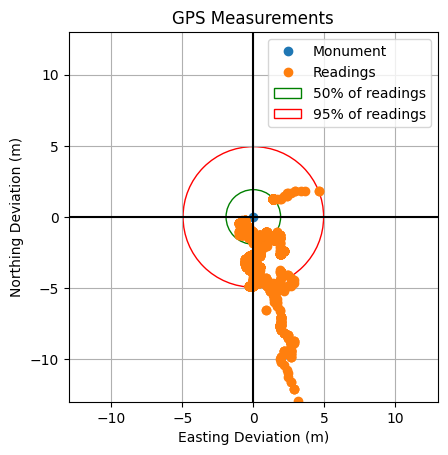
\includegraphics[height=2.5in]{verify_validate/gps_test_errors.png}
\end{figure}

\paragraph*{202 - The system will have a simple human interface accessible via web browser} In earlier versions of the firmware, there was a basic webpage that allowed operators to start/stop logging and check the device status.
However, in the latest firmware version, this capability was removed to simplify testing.
The hardware is still capable of providing this interface but it remains to be implemented.
For more information, see Section \ref{ssec:future_wireless}.

\paragraph*{203 - The system shall be able to monitor and report battery state of charge} This capability has been verified through inspection by integrating the MAX17048 \footnote{\url{https://www.digikey.com/en/products/detail/analog-devices-inc-maxim-integrated/MAX17048G-T10/3758921}} onto the board design.
This chip calculates state of charge and reports it to the microcontroller.
Then the battery state is reported as a battery message through the device API.
However, this capability has not been validated as the battery monitor chip has not been calibrated for the selected batteries nor analyzed for its accuracy.
Further testing is required as detailed in Section \ref{ssec:future_settings} and \ref{ssec:future_vv_power}.

\paragraph*{204 - The system will have configurable settings that can be changed by the operator} This capability was another one that was verified and validated throughout the calibration process by testing.
The firmware implements and extends the xioAPI which provides an extensive list of settings that can be changed via JSON commands \cite{ThetisUserManual}.
The calibration process required tweaks to some settings which were routinely done through the USB connection to a host computer.
Additionally, during development of this feature, every setting was tested and validated to work.

\paragraph*{205 - The system can operate in a Wi-Fi access point or client mode} This capability can be verified by inspecting the manufacturer data sheet for the microcontroller used on Thetis.
The ESP32 series of chips used on the board are Wi-Fi enabled microcontrollers that can broadcast their own networks (access point mode) or connect to a local one (client mode).
On Thetis, switching between these modes and Wi-Fi disabled is done through configuration commands.
Performance of the Wi-Fi connection and other features have not been validated in the latest firmware and should be integrated following the discussion in Section \ref{ssec:future_wireless} and \ref{ssec:future_vv_wireless}.

\paragraph*{206 - The sensor measurements shall incorporate a calibration model} The capability is implemented by using the Madgwick sensor fusion algorithm described in Chapter \ref{chap:background} and the \lstinline[style=customInline]|Fusion| library made for that algorithm.
The \lstinline[style=customInline]|Fusion| library incorporates the calibration model described in Equations \ref{eq:inertial_model} and \ref{eq:magnetic_model} by default and the specific calibration parameters are loaded as configuration settings.
Due to the failure of the calibration process, this capability was not validated.

\section{Stretch Capabilities}

{\fontsize{8pt}{8pt}\selectfont
\begin{table}[ht!]
    \centering
	\renewcommand{\arraystretch}{1.5} % Set row height
	\begin{tabular}{| c | m{0.55\textwidth} | c | c | c |}
		\hline
		\multicolumn{5}{| c |}{\textbf{Stretch}} \\
		\hline
		\textbf{ID} & \multicolumn{1}{c|}{\textbf{Description}} & \textbf{Verified?} & \textbf{Validated?} & \textbf{Status} \\
		\hline
		301 & The system file storage shall be accessible via web or USB interface	& \no & \no & A \\
		302 & The system shall have a backup storage option in case primary storage fails & \no & \no & R \\
		303 & The system will use a microcontroller capable of machine learning using TinyML & \no & \no & UR \\
		304 & The system shall be able to log in a burst mode for up to 24 hours & \no & \no & UR \\
		\hline
	\end{tabular}
	\caption{Verification and validation of stretch capabilities}
	\labtab{vv_stretch_capabilities}
\end{table}
}

\paragraph*{301 - The system file storage shall be accessible via web or USB interface} From previous experiments with the ESP32-S2 and -S3 microcontrollers, it is possible to host a File Transfer Protocol (FTP) server \footnote{\url{https://www.mischianti.org/2020/02/08/ftp-server-on-esp8266-and-esp32}} or have the device appear as a USB flash drive \footnote{\url{https://github.com/Legohead259/ThetisLib/blob/ba94c8f8eba002fef2d88b5f21aa544ef2b5b2b1/Examples/usbmsc/test.ino}} when connected to a host computer.
However, in the latest firmware version, these features are not implemented so this capability is feasible, but not verified or validated in the current system.

\paragraph*{302 - The system shall have a backup storage option in case primary storage fails} This capability was initially envisioned as a mitigation for any microSD card failure mode.
Especially in cases where the microSD card could become physically damaged during a test, the secondary option would still allow some data to be recovered.
However, as explained in \ref{sec:prototype_problems}, this capability introduced system-breaking errors and the anticipated failure mode was never encountered throughout initial testing.
Therefore, this capability was rejected in favor of a simplified and more reliable software and hardware design.

\paragraph*{303 - The system will use a microcontroller capable of machine learning using TinyML} This capability was added to address some of the future efforts proposed in the next chapter.
An experiment was run \footnote{\url{https://github.com/Legohead259/Project-Thetis-TinyML-Example}} that proved the feasibility, but due to the technical effort and time constraints, this capability was not seriously considered for implementation.

\paragraph*{304 - The system shall be able to log in a burst mode for up to 24 hours} This is another capability that was envision for a future use, but never seriously considered for implementation.
The idea with this is to extend the battery life to capture inertial signals over a longer time span such as required for the WEAVE experiment proposed in Section \ref{chap:weave}.
However, this capability could be better implemented by a new hardware revision that could accept external battery power, instead of relying on its smaller internal battery.
Theoretically, this is possible to integrate using the component's sleep functionalities and other techniques.

\section{Stakeholder Requirements}

{\fontsize{8pt}{8pt}\selectfont
\begin{table}
	\centering
	\renewcommand{\arraystretch}{1.75}
	\begin{tabular}{|c | m{0.5\textwidth} | c | c | c |}
		\hline
		\textbf{ID} & \multicolumn{1}{c |}{\textbf{Description}} & \textbf{Verified?} & \textbf{Validated?} & \textbf{Status} \\
		\hline
		SR 01 & The system shall be able to record acceleration, rotation rate, orientation, and position & \yes & \yes & TIP \\
		SR 02 & The system shall be able to fit into a small IP67-rated, or better, enclosure & \yes & \yes & D \\
		SR 03 & The system shall be able to be powered by battery for more than 4 hours continuously & \yes & \yes & D \\
		SR 04 & The system shall be cheaper than \$200 per unit & \yes & \no & A \\
		SR 05 & The system shall use components that are readily available COTS & \yes & \yes & D \\
		SR 06 & The system designs shall be open source for modification by students & \yes & \yes & D \\
		SR 07 & The system shall allow users to change settings via interface and/or configuration file & \yes & \yes & D \\
		SR 08 & The system shall communicate extra-device using WiFi and USB & \yes & \yes & A \\
		SR 09 & They system shall have enough on-board storage for 4 hours of continuously logging at 64 Hz & \yes & \yes & D \\
		\hline
	\end{tabular}
	\caption{Verification and validation of stakeholder requirements}
	\labtab{vv_stakeholder_reqs}
\end{table}
}

\paragraph*{SR 01 - The system shall be able to record acceleration, rotation rate, orientation, and position} The requirement was verified and validated throughout the calibration procedure described in the previous chapter.
Thetis recorded and output the inertial measurements (rotation rate and acceleration), magnetometer readings, position measurements from the GPS, and orientation as both a quaternion and euler angles.
This was recorded through the on-board microSD card logger and through the x-IMU3 GUI application running on a host computer and connected via USB.

\paragraph*{SR 02 - The system shall be able to fit into a small IP67-rated, or better, enclosure} As explained with Capabilities 101 and 102 in Section \ref{sec:threshold_capabilities}, this requirement was verified and validated by testing the enclosure at depth on an ROV and in a more realistic deployment.
The enclosure held a water-tight seal when properly engaged and undamaged.

\paragraph*{SR 03 - The system shall be able to be powered by battery for more than 4 hours continuously} This requirement was verified using the analysis discussed in Section \ref{sec:threshold_capabilities} with Capability 106. 
It was further validated by running the system for more than 4 hours and checking that the end battery voltage was at an acceptable level.

\paragraph*{SR 04 - The system shall be cheaper than \$200 per unit} This requirement was verified by inspecting the Bill of Materials for Thetis and checking that the summation was less than \$200.
This requirement is difficult to validate however, because additional hardware revisions may be necessary to improve performance or add additional features.
This estimate also does not include the development time or overall expense, which would definitely increase the unit price.

\paragraph*{SR 05 - The system shall use components that are readily available COTS} This requirement was verified and validated by sourcing components from online distributors like DigiKey.
All of the components used on Thetis can be purchased online and then assembled on the custom PCB. 
This requirement was tricky to implement during the chip shortage of 2020, but now that more components are more readily available, further hardware revisions should not have any problems continuing to use COTS parts.

\paragraph*{SR 06 - The system shall be open source for modification by students} This requirement is verified by the extensive use of GitHub repositories that are public-facing and accessible by anyone with an internet connection.
Students can access the repositories, download the source code and files, make modifications as needed.
To validate the requirement, multiple groups of students and stakeholders were gathered to attempt various tasks such as repair a chip, calibrate the board, add a new software feature, etc.
As they were performing these tasks, they were given documentation and in turn provided feedback on the quality of the documentation and any clarifications they needed.

\paragraph*{SR 07 - The system shall allow users to change settings via interface and/or configuration files} The requirement was verified by implementing and extending the xioAPI in the Thetis firmware.
This API provides a suite of settings to control how the board performs and its capabilities.
The configurations can be changed via a web or USB interface to a host computer or by uploading a custom configuration file to the onboard flash storage.
To validate the requirement, each setting was thoroughly tested to ensure it could be changed and the interface was used during the calibration process to tweak a couple of settings.

\paragraph*{SR 08 - The system shall communicate extra-device using Wi-Fi and USB} Since Thetis uses a microcontroller that is capable of USB host and Wi-Fi, this requirement is easily verified by inspecting the manufacturer data sheet.
However, the requirement remains unvalidated because the performance when using the wireless interface is severely limited.
More testing is required as detailed in Section \ref{ssec:future_wireless} and \ref{ssec:future_vv_wireless}

\paragraph*{SR 09 - The system shall have enough on board storage for 4 hours of continuous logging at 64 Hz} This requirement was verified and validated throughout the calibration process.
Firstly, the calibration data was captured at 64 Hz proving the second part of the requirement.
Then, as described in Section \ref{sec:threshold_capabilities}, the microSD card storage size was analyzed to ensure that it was large enough and Thetis was run for 4 hours, logging the entire time.
%%-----------------Chapter 6---------------------------
\chapter{Future Efforts and Potential Applications} \labchap{future_efforts}
As you may have noticed, this thesis was an intensive, multi-disciplinary effort that required in-depth knowledge of electronics, board design, software engineering, and systems engineering.
Because of the breadth and depth required by this thesis, some areas were not covered due to technical or temporal constraints.
A large portion of the software was only finalized in the months leading up to finishing this thesis and a hardware fault cost another couple of months of development work.
Therefore, there is a lot left unfinished that is intended for future students to pick up as their own research projects.
Some of these efforts are detailed in this chapter.

\section{Calibration} \labsec{future_calibration}
As discussed at the end of Chapter \ref{chap:calibration}, the calibration procedure failed for the inertial sensors.
The specific reasons could not be determined before the thesis needed to be completed and were out of the technical scope anyways.
Therefore, it will be required in the future to examine these procedures and determine the source of the flaws.

In order to accomplish this, the objective function and constraints should be examined first.
It is likely that the objective function was not used properly with the optimization procedure, producing results that fell into a local minima that satisfied the problem, but did not satisfy the calibration application.
Therefore, the optimization function should be modified to include additional constraints or boundaries to limit the range of ``acceptable'' results from the objective function.
This may improve the accuracy of the calculated misalignment matrices and sensitivity vectors.

Additionally, these procedures should be more thoroughly tested and evaluated across a range of boards and types of sensors.
The calibration script created for this thesis is not sufficient for this task, so the concepts employed by it should be expanded as required.
The measurements can be compared between the boards before and after calibration to determine the efficacy of the proposed procedures.

\section{Hardware Revision F6} \labsubsec{future_hardware}
Based on testing and interviews with Dr. Madgwick \cite{Duffy:2023}, another hardware revision, Revision F6, was created to address some of the concerns with Revision F5.
First, the secondary flash storage chip, the XTSD, was removed entirely since it was redundant and caused the hardware issues that crippled development on Revision F5 for months.

The space created by removing this chip allowed the MARG array to moved to a section of the board that could be mechanically isolated from the rest of the board.
This was necessary because MEMS sensors are affected by strain and in the configuration on Revision F5, the sensors were located at a point of max strain when the board was screwed into the enclosure.
This would affect precision and could cause measurements to slightly vary depending on the torque of the screws used in the assembly.

Additionally, the \lstinline[style=customInline]|data ready| interrupts from the sensors were attached to the microcontroller which should improve performance by switching the measurement method to an interrupt-based one versus polling.
By switching to an interrupt-based measurement method the readings can be taken at a much higher sample rate and be more accurate to the recorded timestamp.
This method is also less computationally intensive on the microcontroller.

Then the microcontroller was changed to one that had an antenna attached directly to its PCB, removing the need for an external antenna.
On the ESP32-S2 microcontroller, the chip would refuse to boot when an external antenna was attached.
This issue was never fully investigated, but the onboard antenna should negate this problem and simplify the overall assembly.

Another change affects the GPS module.
On Revision F5, the ground plane beneath the module was not contiguous and small relative to the antenna size.
This introduced RF noise and attenuation, reducing overall accuracy.
On the new revision, the ground plane is stitched together with vias linking the top and bottom planes.
This should improve performance slightly over Revision F5.

Finally, the power supply was substituted for a more efficient DC-DC converter which should improve efficiency and extend battery life.

This revision has been designed in ECAD, but was not ordered or built due to time constraints.
Therefore, in the future, a student or group of students can build and verify and validate this design using the procedures laid out for Revision F5.

\revisionfigure{f6}

\section{Software Improvements} \labsec{future_software}
There are several things that are feasible with the hardware available that were not able to be implemented before the thesis needed to be completed.
Most of these features are not explicitly required by the system requirements, but they could improve the quality and usability of Thetis.
These improvements are being tracked in the Thetis project on GitHub\footnote{\url{https://github.com/users/Legohead259/projects/1}}.

\subsection{Wireless} \labsubsec{future_wireless}
Thetis currently struggles with sending data wirelessly to a host computer.
The only protocol supported is the Universal Datagram Protocol (UDP) which is the simplest internet protocol (IP) to implement.
Packets of data are blasted out with a header denoting the target IP address and port with no regard to signal strength or if the target receives the packet.
This is the most efficient method as there is no handshaking or acknowledgement protocol to saturate the limited bandwidth and compute cycles.

However, as currently implemented, the process takes far to long to format a packet and send it to the target, resulting in a 90\% drop in overall sensor sample rate.
I believe the implementation of the \lstinline[style=customInline]|UDPServer| class is to blame, but more thorough research needs to be performed.
For Thetis to be more effective for the operator, the UDP service should be fixed so that it performs adequately when wirelessly streaming data to a host computer.

Additionally, Thetis cannot handle with the x-IMU3 GUI first connects to it over UDP.
The GUI application broadcasts over 70 requests for settings data simultaneously when first connecting or reading/writing settings which overloads the UDP client buffer on Thetis.
This means that GUI cannot establish proper communication with the device and cannot change settings wirelessly.
Again, to improve its effectiveness and ease of use, this should be fixed.

For deployments, it would also be preferred if the logging and status could be monitored remotely.
This can be done by incorporating a basic web server into Thetis that shows an HTML page with a button for starting/stopping logging and a status box that mimics the on board LED.
Some system information such as time and sensor health could also be presented to the operator for easier diagnostics.
An example can be found in older versions of the firmware.\footnote{\url{https://github.com/Legohead259/ThetisLib/blob/d5982b721212952777a11934ff837b62f7591226/src/radios/wifi.cpp}}.

\subsection{Settings/API} \labsubsec{future_settings}
The settings used on Thetis follow the xioAPI specification which is a set of key/value pairs.
Some of these settings need to be accessible on the device, but should not be overwritten (i.e. factory-settable only).
Currently, Thetis' firmware does not protect these settings and does not support a factory program mode.
This means that at any time, crucial settings like the calibration parameters, serial number, etc. can be overwritten by the user or a host application.
This commonly occurs with the x-IMU3 GUI application which writes blank strings and zero arrays and zero matrices for some factory settings.
When Thetis is connected to the GUI and settings are written to it, a lot of features are temporarily broken until the default values can be restored.
This needs to be fixed to improve the interaction with the operators.

Some settings are also not fully implemented when they should be or they are only implemented at start up.
For example, settings related to sensors such as sensitivity and sample rate are configured when the system first boots.
If these settings are changed during operation, the system must be reset for them to take effect.
This can be streamlined by having callback functions for updating system settings when a new configuration is received.

Several message also need to be implemented, like the battery message.
This will allow the log file to record the battery state over time and may aid with power verification and validation.

\subsection{Data Storage} \labsubsec{future_data}
Currently, the data log recorded to the microSD card is a generic ``logXXX.bin'' where $XXX$ is a three-digit number that is one larger than the previous log file.
While simplistic to implement, this method makes tracking down specific log files difficult as the operator must track the number of times the system is restarted or reset, or the projected length of the log file.
The settings already support custom log file names and prefixes and suffixes, so these should be implemented fully to make logging easier.
Also, the file name extension should be changed to ``.log'' or something similar.

The firmware should also be updated so that the microSD is accessible via different methods.
First, Thetis should show up as a USB flash drive when connected to a host computer.
Files can be transferred over the USB connection without removing the microSD card.
Second, the filesystem should be accessible over a FTP service where operators can wirelessly log in and copy/remove files.
This will be very useful for deployed applications where Thetis cannot be easily opened or physically accessed.

\subsection{Sensors} \labsubsec{future_sensors}
Many of the sensors implemented in the firmware are based upon the Adafruit libraries for those components.
While this simplifies the integration, it bloats the memory and storage requirements.
This also creates a dependency on third-party software which could be problematic in some situations.
Therefore, it would be nicer to have all of the sensors packaged individually in libraries that are self-contained and conform to the I2CDevLib\footnote{\url{https://www.i2cdevlib.com/}} standards.
This would improve the code performance and reduce memory requirements.

Additionally, the \lstinline[style=customInline]|Fusion| library has implemented some new features for accelerometer and magnetometer rejection and status flags that would be useful for the entire sensor fusion process.
Therefore, the firmware should be migrated to this new version and have these features implemented.

If the hardware is migrated to Revision F6, the sensor polling method should also be swapped out for an interrupt-based approach.
Instead of asking the sensors every period what their data is, the method must change to asking as soon as a pulse is received on the ``data ready'' input pins.
This will make computation more efficient and allow for high sampling speeds.
Also, the divisor settings can be implemented here to automatically average $N$ number of samples before reporting it.

\section{More Verification and Validation} \labsec{future_vv}
Identifying and fixing a major design flaw with Thetis Revision F5 occupied a large amount of time that could have been used to further verify and validate some features.
Unfortunately, that means there are still some things to be analyzed before the design can be considered ``100%'' completed.

\subsection{Wireless} \labsubsec{future_vv_wireless}
The wireless features of Thetis need to verified by proving that data and settings can be streamed from the device to the host computer over a UDP connection.
This should be done in both access point and client modes to cover the breadth of use cases.
Of course, before these tests can be done, the problem with the UDP server and client should be addressed.

It is also important to characterize the strength, speed, and bandwidth to understand the limits of the wireless features.
To test the signal strength, Thetis should be enclosed in its container and then set to wireless access point mode.
A smartphone with the appropriate application can then detect the Thetis access point and will report its strength.
Move the phone several distances away from the access point and plot to get a rough characteristic.

Similarly, Thetis can be placed into the wireless client mode and connected to a local access point.
Assuming the message is implemented in the firmware, Thetis can report the wireless signal strength and log it.
Again, move Thetis given distances away from the access point and plot to roughly characterize it.
The connection speed and bandwidth can be tested by running files of a known size through the FTP service and recording the amount of time to transfer the data.
Ideally, there will be decent strength out to about 10-meters and the file transfers will occur within a minute or two.

\subsection{Power} \labsubsec{future_vv_power}
The verification and validation for power described in this thesis was just ``does it last four hours or not''.
It is important to fully characterize the power draw so that the operator can know the limits of the device.
Additionally, measuring the power draw during certain operation modes can identify points for improvement and the hardware or software can be modified to increase battery life.
The devices can also be put into a sleep mode (assuming that is supported in the firmware) and power consumption characterized.
With the normal operating mode and sleep mode consumptions known, it will be possible to set up a burst measurement mode to increase deployment life, if desired.

\section{Calibration Machine} \labsec{future_calibration_machine}
Calibrating Thetis is currently a manual process that is prone to errors from the procedure and the testing apparatus.
For example, in the gear apparatus for calibrating the accelerometer and orientation, the calibration cube could accidentally be misplaced by a single tooth, causing a deviation of 5-degrees.
This may not be immediately caught, introducing errors.
To automate the process and reduce potential errors, an expansion upon the current calibration machine is proposed which incorporates more features to improve usability.

\subsection{Requirements} \labsubsec{future_cm_requirements}
In order to effectively automate the process and reduce the chances of human error, the machine should be able to rotate the IMU about all three-axis on its own and in a controlled manner.
Additionally, each of these rotations should be tracked with an absolute position sensor to understand the IMU's position and rotational velocity to a high degree of accuracy.
The most compact way to accomplish this may be to borrow the design from a three-axis camera gimbal using high torque brushless DC motors, as shown in Figure \ref{fig:three_axis_gimbal}.

\begin{figure}
    \centering
    \caption[Three Axis Gimbal]{The rear of a three-axis gimbal used on UAVs for action cameras. 
    Courtesy of RC Product India. \url{https://www.rcproduct.in/product/feiyutech-oem-sftuav-mini-3d-3-axis-gimbal/}}
    \labfig{three_axis_gimbal}
    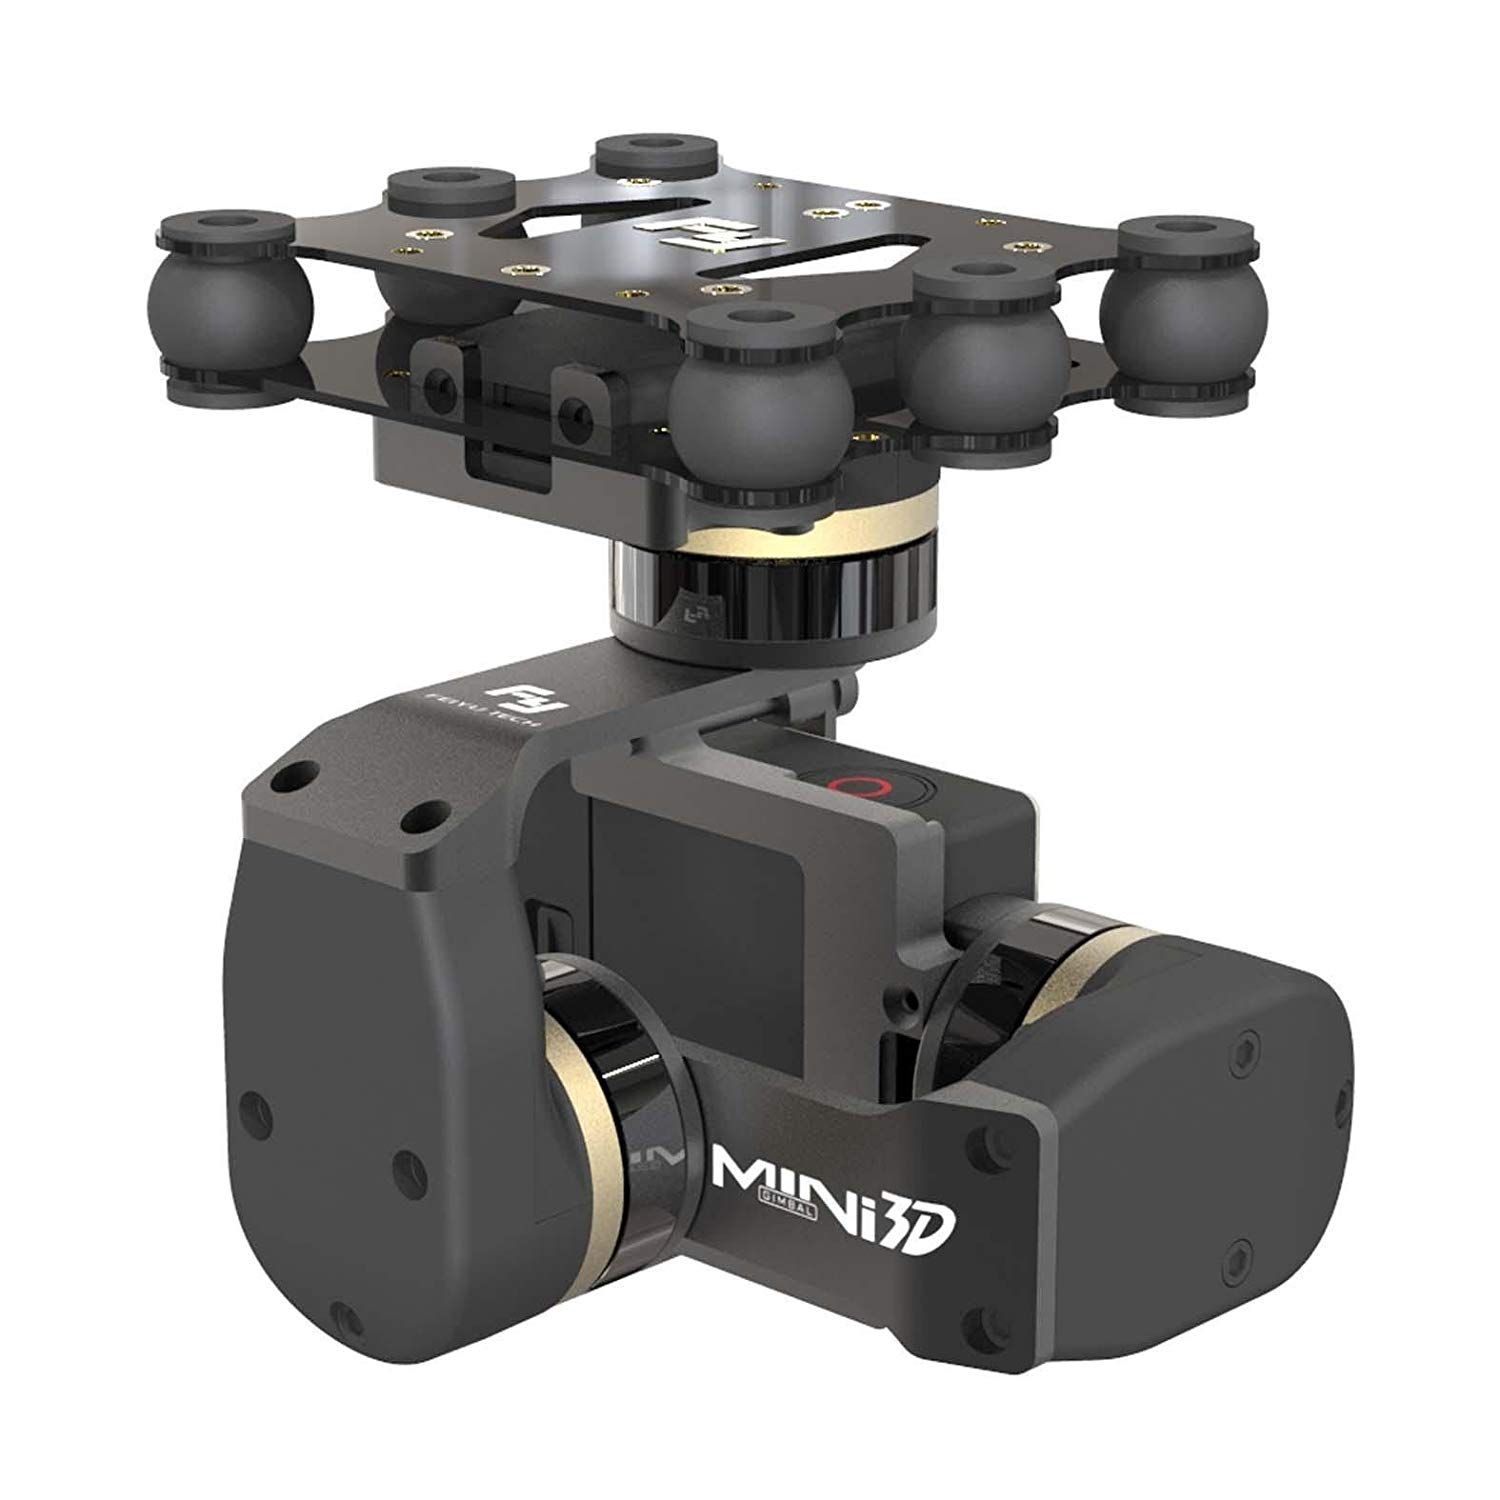
\includegraphics[height=2in]{future_efforts/three-axis-gimbal.png}
\end{figure}

Controls for the motor need to happen in near real-time and the main computer should also be able to send commands and data around the system quickly and efficiently.
This can be accomplished with a Data Distribution Service (DDS) topology that incorporates publish/subscribe and client/server interactions.
The most popular framework for this type of network is ROS2, which is used on the current calibration machine and should be able to modified to a new platform.
The new calibration machine should also be open architecture such that new IMUs with different communication methods or new calibration sensors can be quickly integrated.

Finally, the main controller for the new machine should be powerful enough and have enough storage access to build a database with the calibration and validation results.
Ideally, this controller would also have access to the Internet so that the information could be published to a cloud database for more accessibility.
It would also be prudent to have the controller in a headed configuration with a simple touchscreen user interface to start/stop the procedure and monitor the system status.

\subsection{Block Diagram} \labsubsec{future_cm_block_diagram}
To meet the proposed requirements, the hardware block diagram in Figure \ref{fig:calibration_machine_v2} is introduced.
The core of the machine is a Raspberry Pi microcomputer that would be running Ubuntu with ROS2 loaded onto it.
A Hardware Attached on Top (HAT) daughter board would be attached and responsible for handling the sensor inputs, motor driving, etc.
The Pi would be connected to an official 7-inch touchscreen as a human-machine interface (HMI) and then connected to a local area network (LAN) for connectivity features.

The motors for the gimbal would have a diametrically magnetized magnet on the shaft with a magnetic compass placed beneath it.
As the magnet moves, the compass can detect the rotation direction and speed.
By determining a ``home'' position, the compass can also detect the degrees rotated from an arbitrary zero point.
This allows ground truth measurements to be taken for the gyroscope, accelerometer, and orientation datasets for all three rotation axes.
A microcontroller can be placed on the Raspberry Pi HAT and handle the real-time control of the motors and sensors, while interfacing with the Pi over a serial port such as UART, SPI, or I2C.

[TODO: Insert block diagram for calibration machine]

The data can be run through the ROS2 packages and a master script can analyze the data at the end of the calibration process and produce the results.
Then, the same can occur after the validation process and a calibration certificate can be made that shows the IMU error over all the testing regimes.
This architecture is represented in the block diagram in Figure \ref{fig:calibration_machine_ros}.

[TODO: Insert block diagram for the ROS2 architecture]

\subsection{Concept of Operations} \labsubsec{future_cm_conops}
For the new calibration machine, the idea is a one-touch solution that is fully automated, requiring minimal human intervention.
At the start of the test, the operator can press the ``Start'' button and the machine will home each axis to a zero point and begin calibrating the accelerometer and gyroscope.
Each axis will be individually rotated in 45-degree increments for a complete revolution.
Then, they will be rotated at a few target speeds.
Simultaneously, the IMU will be streaming data to the Raspberry Pi for collection and processing.
After the accelerometer and gyroscope datasets are collected, the IMU will be simultaneously rotated about all three axes to collect the magnetometer calibration dataset.

When these steps are completed, the master script will compute the calibration parameters and upload them to the IMU's sensor fusion algorithm.
Then, restart the testing procedure with finer increments to increase the number of validation data points collected.
After the sensor validation datasets are collected, the machine will rotate the IMU into various poses as part of the orientation validation dataset.
Finally, the master script will process the validation datasets into a single calibration certificate product that the operator can view.

While the entire process is occurring, crucial data will be shown on the screen to the operator along with an ``ESTOP'' button.
If the machine detects an error, or the human operator wants to stop the test, there will be a set of commands to safely shutdown the system.
Additionally, the machine will have several settings that can be tweaked by the operator prior to a calibration run - like the gimbal zero positions.

\section{Floating Body Testing} \labsec{future_testing}
The original intent of Thetis was to supplement class resources in the Ocean Engineering department.
Naturally, this means that Thetis should be used in Ocean Engineering applications by students.
Instructors may also find Thetis useful for their research as it is a small and cheap platform, perfect for a proof of concept experiment that could lead to larger revelations.

\subsection{Surfboard} \labsubsec{future_testing_surf}
The first application is in the Surf Engineering Analysis or Ocean Engineering Data Analysis course.
Here, students will put Thetis into a surfboard and paddle out into the ocean surf to catch some waves.
Thetis' sensor suite will provide students data on the board's orientation, acceleration, velocity, and position in the local and global coordinate frames which they can use as part of their class project.
Thetis improves upon the sensors used for that course by having a larger sensor suite and a better sensor fusion algorithm to process the data.
It would also be interesting to put the x-IMU3 into the same board and environment and see how they compare.

\subsection{Model Barge} \labsubsec{future_testing_barge}
Another application is with the fluids laboratory or a naval architecture laboratory section.
Currently, one lab experiment performed by students is the analysis of a vessel's movement based on weight placement and metacentric height.
The model barge is equipped with inclinometers for the pitch and roll that students must analyze time step by time step to create a plot of the roll/pitch.
Typically, this is done after the experiment doing frame-by-frame video analysis.
If the video is blurry, or the vessel yaws during the test, this analysis can be difficult and time-consuming.

To simplify the process, Thetis can be placed on the barge and set to record the vessel's orientation at a much high frequency than a frame-by-frame analysis and more accurately.
The data can also be stream wireless in real-time to a host computer that would allow the instructor to more dynamically and visually demonstrate the effect of metacentric height on vessel stability.
This can also be done to larger scale vessels in a larger tank or in a class room.

\subsection{WEAVE} \labsubsec{future_testing_weave}
The last major application considered is the proposed Wave Estimating Algorithm for Vessels Experiment, or WEAVE.
Based on the floating model barge experiments and previous work done in \cite{Gait-Tracking}, WEAVE is an exciting study into an alternative method for wave characteristic measurement.
Thetis can be placed on top or within a wave buoy and deployed on the ocean.
While there, it can record the inertial characteristics of the buoy which can be used to determine the wave parameters over time.
The parameters can be calculated in both the time and frequency domains which would be compared to the ground truth from the wave buoy.
For more information, a more in-depth whitepaper manuscript is presented in Appendix \ref{chap:weave}.
\chapter{Conclusion} \label{chap:conclusion}
A low-cost, low-profile inertial data logger was designed, tested, and validated throughout this thesis.
I set out to design the board as a solution that students could use in their projects in and out of the classroom and as a replacement for some of the current equipment.
In putting the board together, I did my best to learn and follow system engineering best practices for a small embedded device like this and thoroughly validate the design before delivering it.
There were some problems, a couple of hiccups, and one or two or three major disasters along the way, but ultimately Thetis works.
It is an all-in-one datalogging solution, that is beneath \$200 in cost, is open source and publicly available, and is capable of recording inertial characteristics in 9 degrees of freedom with a GPS radio providing positional fix.

By reading through this thesis we have considered the two research questions posed in the introduction.
We have learned how inertial measurement units work, and we have learned how we can design our own instrumentation board to capture and report those readings.
With the capabilities found in Thetis, we can now move on to larger experiments incorporating it and continue to innovate in the research field.
All the while remembering to teach the next generation everything we know and providing them a platform to exceed us.

%% -----------Back Matter---------------------------
%% -----------Bibliography--------------------------
\nocite{*}
% Do not split a reference between two pages, this should be taken care of in the style
% \bibliographystyle{plain}
% \bibliography{mybibliography}
\printbibliography

%% -----------Appendices----------------------------
\appendix
\chapter{Voltage Divider} \labchap{voltage_divider}
The most basic way to measure resistance is with a voltage divider.
A voltage divider consists of two resistors in series that go between an input voltage and ground, as shown in the schematic below.
The resistive sensor is placed at the $R_2$ position and we want to read the potential between the top of $R_2$ and ground, $V_{out}$ to determine the sensor's resistance.
This voltage can be determined by the equation:

\begin{equation} \labeq{voltage_divider}
    V_{out} = V_{in} \frac{R_2}{R_1 + R_2}
\end{equation}

\begin{figure}[h!]
    \caption{A typical voltage divider circuit}
    \labfig{voltage_divider}
    \centering
    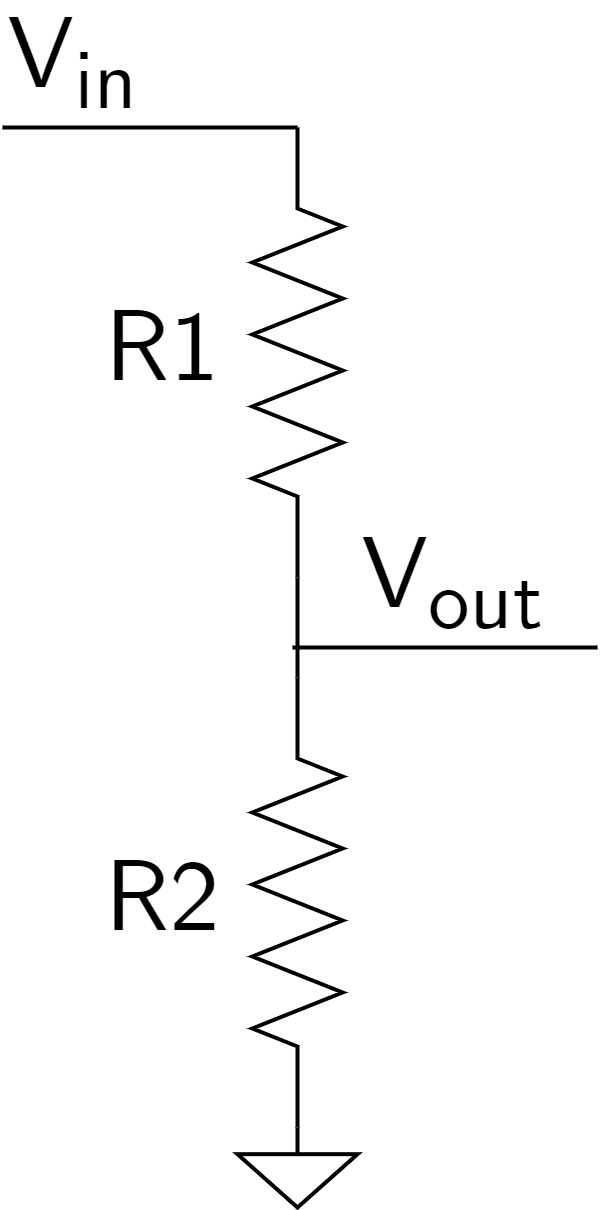
\includegraphics[height=2.5in]{appendices/voltage_divider/voltage_divider.png}
\end{figure}

\section{Example: Battery Monitor}
Let's say a device uses a 3.3V-logic microcontroller.
It can only accept signals up to 3.3V before risking damage to its circuits.
If you want your device to be portable, you can use a lithium polymer (LiPo) battery, but these must be carefully monitored to prevent over discharge.
A single-cell LiPo battery has a peak voltage of 4.2V which is higher than what the microcontroller can handle.
So, we must step down the voltage such that the peak battery voltage matches the peak input voltage of the microcontroller. \\

This is a perfect application for a voltage divider, but we must first determine what two resistors will be used.
To linearize (simplify) the problem, we will arbitrarily set $R_2 = 10\text{k} \Omega$.
Then, we can rearrange the problem to solve for $R_1$

\begin{align*}
    V_{out}                 &= V_{in} \frac{R_2}{R_1 + R_2} \\
    \frac{R_2}{R_1 + R_2}   &= \frac{V_{out}}{V_{in}} \\
    R_1 + R_2               &= \frac{V_{in} \cdot R_2}{V_{out}}\\
    R_1                     &= \frac{V_{in} \cdot R_2}{V_{out}} - R_2 \\
                            &= \frac{4.2 \cdot 10\times10^3}{3.3} - 10\times10^3 \\
    R_1                     &= 2727 \Omega
\end{align*}

To get a resistor that is exactly 2727 $\Omega$ is very difficult, but we can approximate this value using the much more common 2.7 k$\Omega$ resistor without introducing much error into our measurements.

\begin{figure}[h!]
    \caption{A simple battery monitor circuit for 3.3V logic level microcontrollers.}
    \labfig{battery_monitor}
    \centering
    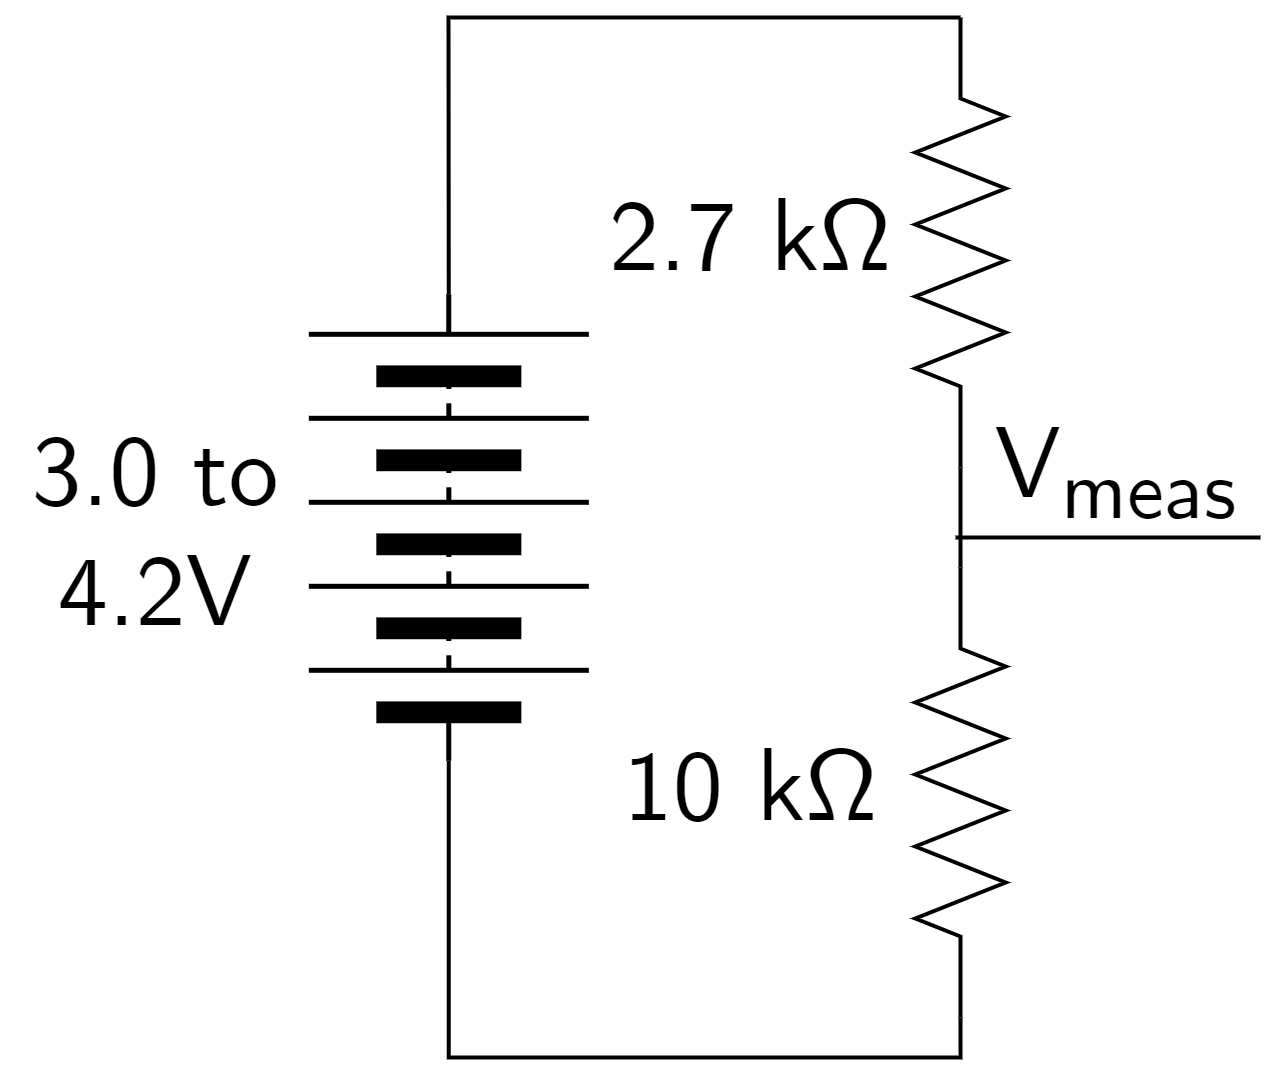
\includegraphics[height=2.5in]{appendices/voltage_divider/battery_monitor.png}
\end{figure}
\chapter{Wheatstone Bridge} \labchap{wheatstone_bridge}
The Wheatstone Bridge is a configuration of four resistors in two voltage dividers, as shown in Figure \ref{fig:wheatstone_bridge}, that is sensitive to minute changes in resistance.
Resistors $R_1$ and $R_2$ form the first divider and $R_3$ and $R_4$ form the second divider.
The bridge has at least three different solutions, depending on the configuration and desired application.
For applications where $R_1$, $R_2$, and $R_3$ are known to a high precision, then $R_4$ can be determined to an equally high precision by adjusting $R_3$ until the voltage potential between points $B$ and $D$ is near 0, i.e. the bridge is ``balanced''.
However, for most embedded applications, $R_4$ cannot be determined by balancing the bridge, so either the general solution or linearization must be used.
For simplicity, only the linearization solution will be examined here.

\begin{figure}[h!]
    \caption{A generalized wheatstone bridge}
    \labfig{wheatstone_bridge}
    \centering
    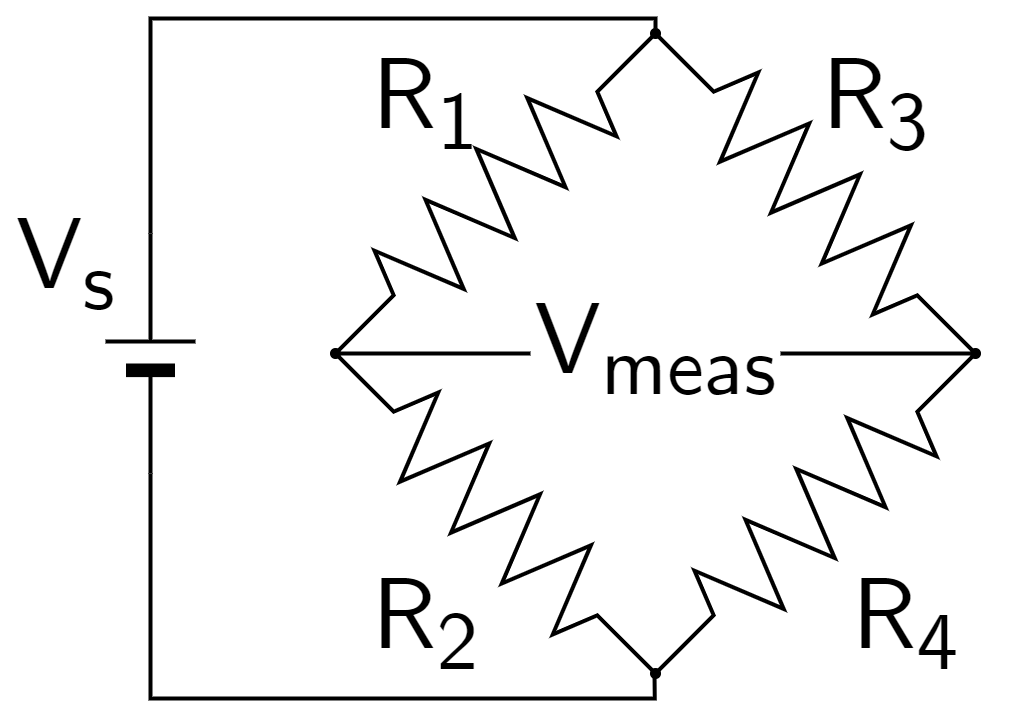
\includegraphics[height=1.5in]{appendices/wheatstone_bridge/wheatstone_bridge.png}
\end{figure}

For the linear solution, the circuit adds an operational amplifier between points $D$ and $B$ and assumes that $R_1=R_2=R_3=R_0$ and $R_4 = R_0 + \Delta R$ and the op-amp is an ideal component ($R_{\text{amp}}$ = 0).
Because of this, the voltage potential at Point $B$ will have a constant value of:

\begin{equation*}
    V_B = \frac{R_0 V_s}{R_0 + R_0} = \frac{V_s}{2}
\end{equation*}

\begin{figure}[h!]
    \caption{A linearized wheatstone bridge}
    \labfig{wheatstone_bridge_linearized}
    \centering
    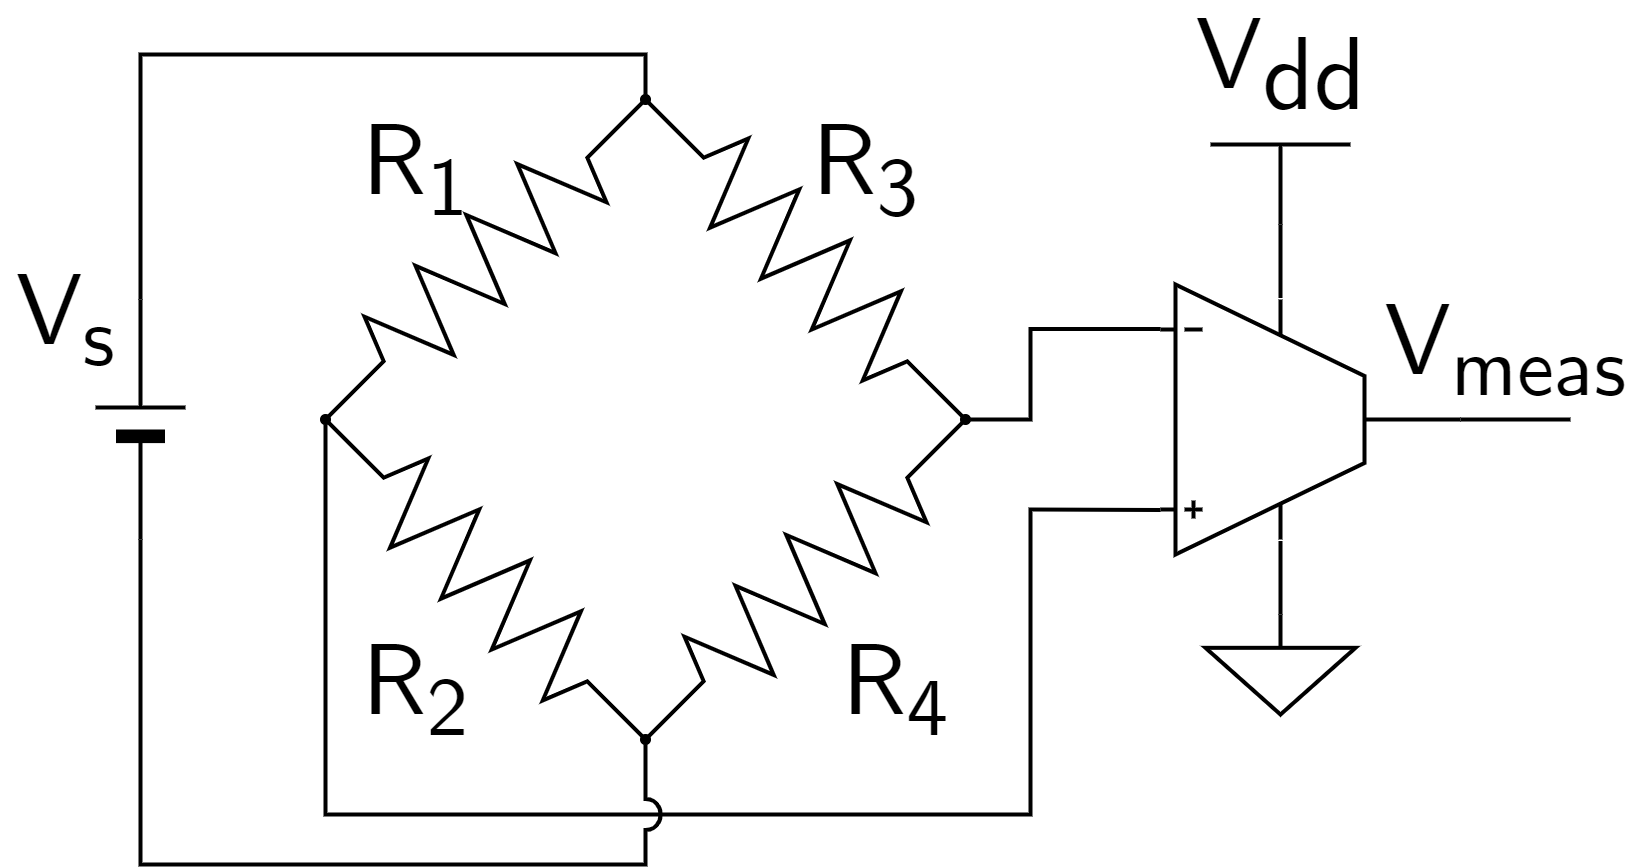
\includegraphics[height=1.5in]{appendices/wheatstone_bridge/wheatstone_bridge_linearized.png}
\end{figure}

Likewise, the op-amp will force the voltage at Point $D$ to have the same voltage as $B$ such that, $V_D = V_B = \frac{V_s}{2} $.
This forces a constant current of $\frac{V_s}{2R_0} $ through $R_3$ and into the sensor.
By Ohm's law, the voltage across the sensor will therefore be:

\begin{align*}
    V_4 &= \frac{V_s}{2R_0} \cdot R_0(1+\Delta R) \\
        &= \frac{V_s}{2} + \frac{V_s}{2} \Delta R
\end{align*}

By applying Kirchoff's voltage law, the potential between the amplifier output and ground, $V_{out} $, is:

\begin{align*}
    V_{\text{meas}} &= -V_4 + V_D \\
            &= -\left( \frac{V_s}{2} + \frac{V_s}{2} \Delta R\right) + V_D \\
    V_{\text{meas}} &= -\frac{V_s}{2} \Delta R
\end{align*}

The measured output voltage now linearly changes with the resistive sensor irregardless of if the sensor changes linearly itself.
If the manufacturer of the sensor provides a table or equation that relates the sensor resistance to a real-world value, we can find the sensor resistance via:

\begin{align*}
    R_4 &= R_0 + \Delta R \\
        &= R_0 - \frac{2V_{out}}{V_s}
\end{align*}
\chapter{Analog Measurement} \labchap{analog_measurement}
In electronics, there are two different types of signals: digital and analog.
Digital signals are either a ``high'' voltage, or a ``low'' voltage, representing either a logical 0 or logical 1.
These signals are great for threshold measurements such as ``is there a cart present at the start of the ride, yes or no?'', but cannot express a range of values.
Conversely, analog signals are better suited to expressing real-world values that naturally vary from a minimum to a maximum and can be any value in between.
Thus, analog signals are prevalent for devices that measure ``real'' things such as speed, acceleration, rotation rates, barometric pressures, etc.

\begin{figure}[h!]
    \caption[Analog versus digital waveforms]{A digital square wave (top) versus an analog sinusoidal wave (bottom).
    Courtesy of SparkFun \cite{SparkFun:AnalogDigital}}
    \labfig{analog_vs_digital}
    \centering
    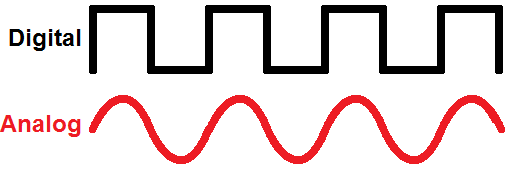
\includegraphics[width=0.5\textwidth]{appendices/analog_measurement/analog_vs_digital.png}
\end{figure}

Most analog sensors are resistive types where their electrical resistance changes to scale with a real-world measurement range.
Ohm's Law defines the relation between voltage, ($V$) resistance ($R$), and current ($I$) as $V=IR$.
Therefore, if we can measure the voltage drop across a resistive sensor and correlate it with a manufacturer-provided equation or table, we can quantify a real-world phenomenon.
The resistance is best measured using a Wheatstone Bridge and an amplifier which can generate a voltage that is directly proportional to the change in resistance, $\Delta R$

\section{Analog to Digital Conversion} \labsec{analog_to_digital_conversion}
Now that we can get a sensor reading as an analog (changing) voltage, we need to find a way to translate it into a useful form.
Decades ago, the analog voltage from a sensor was plotted onto a chart with respect to time and an analyst could run the conversion point by point.
In a real-world experiment, it would be very difficult to deploy a large plotter to capture field data.
We also want to work smarter and not harder, so we want a computer to perform the analysis for us. 
What can we do?
Since we live in the digital age, we can convert the analog signal to a digital one and then we can store it on a digital media device such as an SD card then load it directly into a computer program like Excel to analyze it.

This process is done with an analog to digital converter circuit or ADC. 
The ADC samples an analog waveform at a given frequency and places the voltage level into bins for each measurement.
There are $2^N$ bins in an ADC depending on its resolution, $N$.
For each measurement, the ADC will also encode the voltage reading as a binary number and save it to a register.

This encoded binary number is expressed as ``counts'' which can be read by a microcontroller or other digital system.
The number of counts recorded can be converted back to a voltage value at any time using the equation below.
However, this conversion will lose some of the original precision of the analog signal, depending on the resolution of the ADC.
A higher resolution will mean a more precise reading.

\begin{equation*}
    V = V_{\text{s}} \frac{\text{counts}}{2^N}
\end{equation*}

\begin{figure}[h!]
    \caption[Analog to digital converter waveform]{A 3-bit ADC waveform converting an analog sinusoidal voltage wave (red) of period, $T$, to a digital representation (black).
    Each ADC bin is shown by a blue dashed line.}
    \labfig{adc_wave}
    \centering
    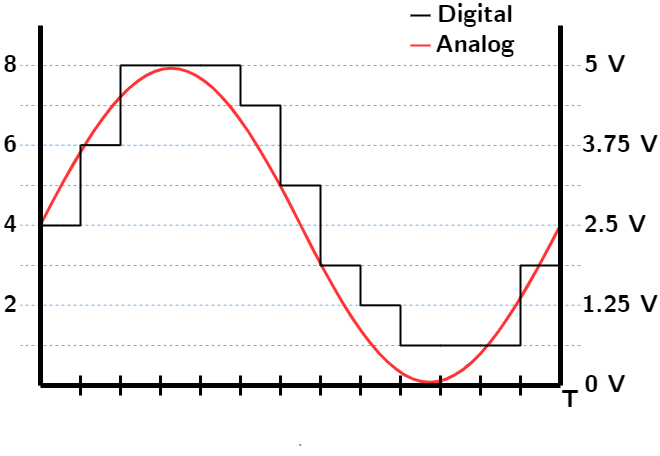
\includegraphics[height=2.5in]{appendices/analog_measurement/adc_wave.png}
\end{figure}

\begin{figure}
    \centering
    \begin{fitbox}[frametitle=Aside: Registers]
        Digital values are stored in memory as 1's and 0's.
        Each bit of memory can be stored in a contiguous piece called a ``register''.
        A digital system can access registers of memory to grab values and perform calculations on them.
        For example, an 8-bit ADC will store the encoding of an input signal in an 8-bit register.
        A microcontroller can then read this value from the ADC and convert it to a real-world value, or save it to non-volatile memory for logging.

        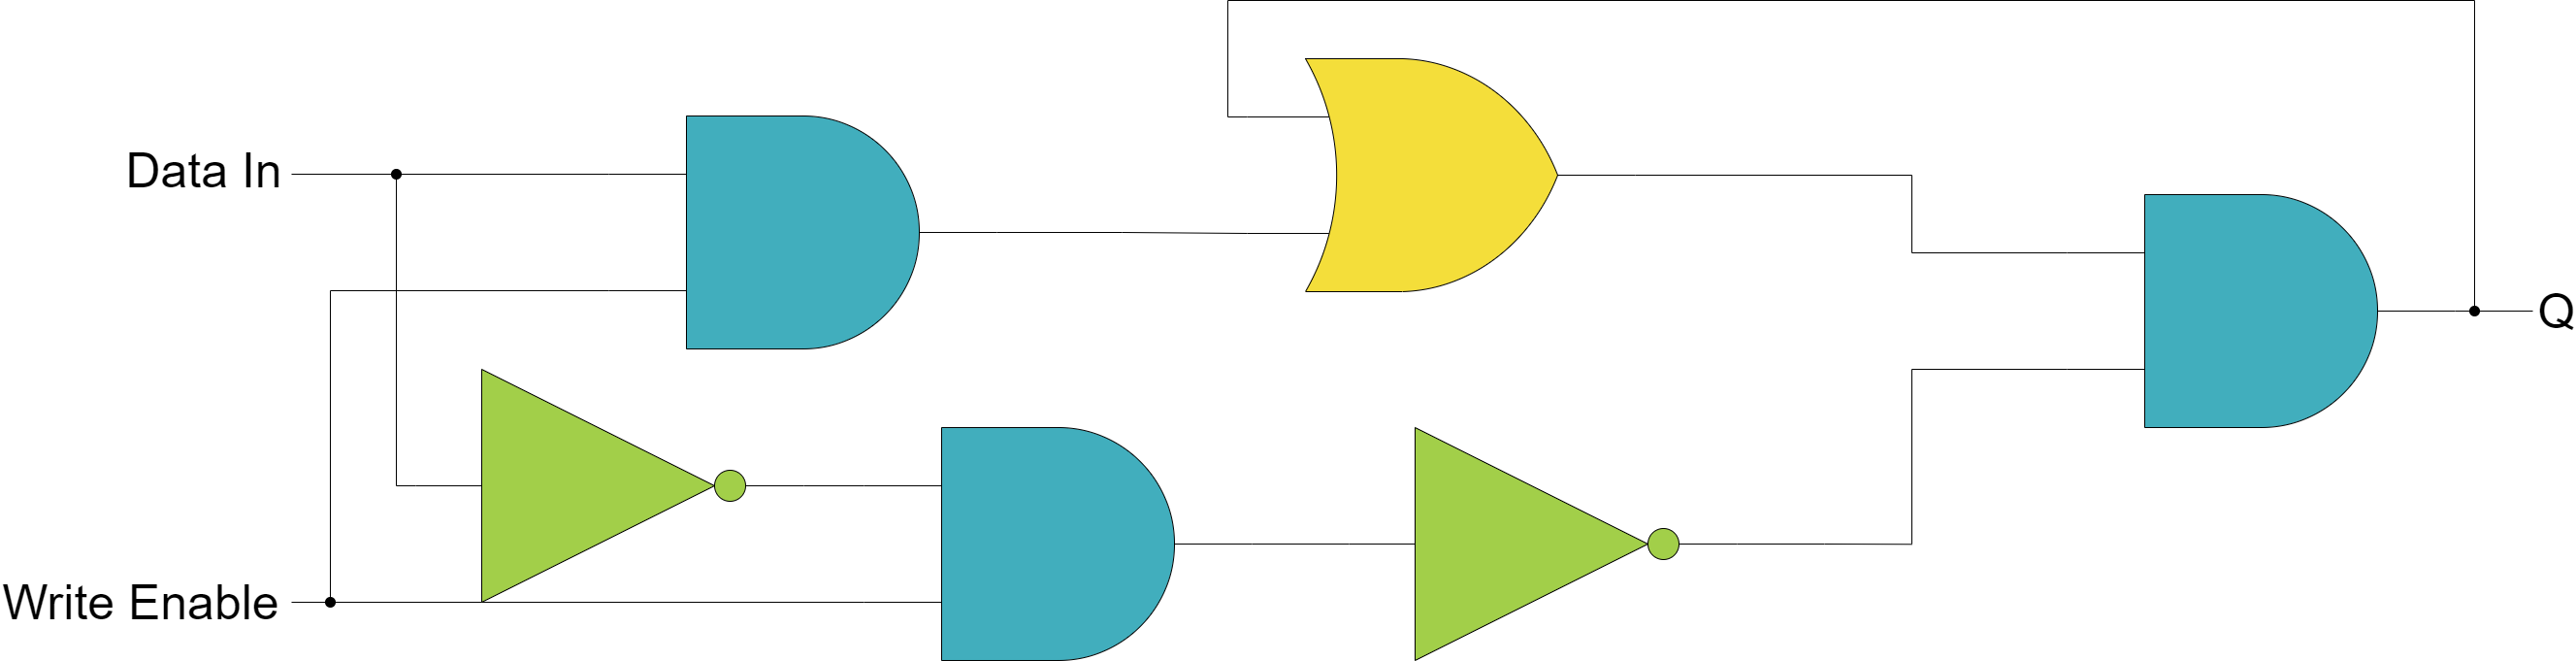
\includegraphics[width=\textwidth]{appendices/analog_measurement/gated_latch.png}
        \caption{A gated latch circuit used to store 1 bit of memory.}
    \end{fitbox}
\end{figure}
\chapter{Digital Communication Methods} \labchap{digital_communications}
Now that we have converted the analog sensor reading into the digital realm, we have to move the data around to use it.
There are many communication methods that utilize a variety of protocols, but for simplicity we will be discussing three of the most common in small digital circuits.
Each of these methods utilize ``Transistor-Transistor-Logic'' or TTL voltages, meaning the signals use 0V for a logical 0, and any other voltage above a threshold is considered a logical 1.
Each method is also known as a serial communication method as each bit in the message is communicated in series.

\section[UART Explained]{Universal Asynchronous Receive and Transmit} \labsec{uart}
The Universal Asynchronous Receive and Transmit (UART) bus is a full-duplex digital communication method where the receiver and transmitter of information can transmit asynchronously. 
This is one of the simplest communication interfaces as a controller only needs to pull the data bus to the ``low'' state at certain intervals while transmitting.
There is no addressing or synchronization required, so the transmitter can just ``shout'' the bits down the line and does not care if the receiver gets them or not.
Since its asynchronous, both the receiver and transmitter must agree on the baudrate, or bits-per-second, beforehand and will set their own internal clocks to the appropriate speed.
By timing the arrival of ``low'' or ``high'' signals, the controllers can interpret data in the transmission packet.
If the baudrates are not synchronized properly, the interval between the bits will be different and data will become corrupted at either end.
Further reading can be done at Analog Dialogue \cite{AnalogDialogue:UART}.

\begin{figure}[h!]
    \caption[UART protocol diagram]{The UART protocol diagram with a small waveform example. 
    Courtesy of Eric Pena and Mary Grace Legaspi \cite{AnalogDialogue:UART}.}
    \labfig{uart_protocol}
    \centering
    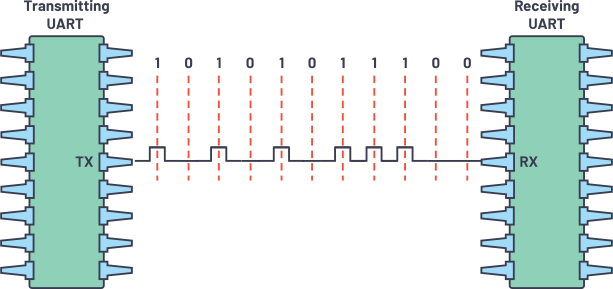
\includegraphics[height=2.5in]{appendices/digital_communication/uart_protocol.png}
\end{figure}

\section[I2C Explained]{Inter-Integrated Circuit} \labsec{i2c}
The I2C, or Inter-Integrated Circuit, communication bus is most commonly used for slower speed transmissions between integrated circuits on a circuit board.
It is a synchronous, multi-nodal, half-duplex topology which means that multiple controllers and responders can exist on the same bus and communicate, but not simultaneously.
I2C uses two pins for communication, one for data (SDA) and one for clock (SCK).
Unlike UART, I2C devices do not need to agree on a clock speed before communication begins, the clock line speed is adjusted by the controller and all devices automatically synchronize to it.
Additionally, I2C devices have a one-byte address that distinguish them and allow for a controller to request data from a specific responder.
This limits the number of unique devices on an I2C bus to 255 and can create some problems if multiple I2C devices of the same address are present.
For the latter problem, I2C multiplexing solutions exist to mitigate the issue \footnote[3]{https://www.adafruit.com/product/2717}.

To begin a message, the controller will initialize a start condition on the line then broadcast the desired device address.
This lets all devices on the bus know that the controller wants to talk with a specific device.
The controller will then follow-up with a one-byte data frame.
Depending on the responder's programming, it will respond with another data frame that the controller will receive.
a typical example of this is a controller querying a device for the value of a register in its memory.
Further reading can be done at Analog Devices \cite{AnalogDevices:I2C}.

\begin{figure}[h!]
    \caption[I2C protocol diagram]{The I2C protocol diagram with a successful write byte transmission. 
    Courtesy of Sal Afzal \cite{AnalogDevices:I2C}.}
    \labfig{i2c_protocol}
    \centering
    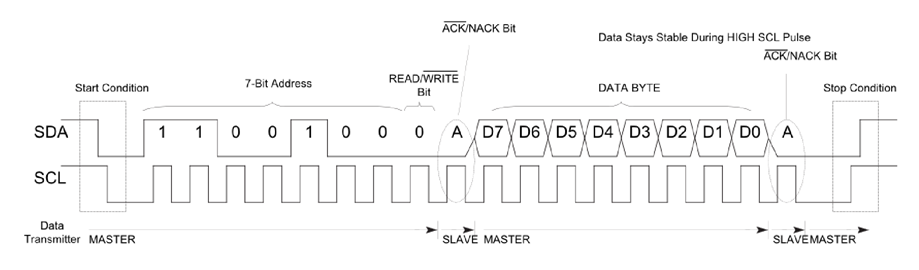
\includegraphics[width=\textwidth]{appendices/digital_communication/i2c_protocol.png}
\end{figure}

\section[SPI Explained]{Serial Peripheral Interface} \labsec{spi}
The Serial Peripheral Bus (SPI) is the slightly modified version of the UART protocol.
SPI introduces clock synchronization so that a main and subnode do not have to agree on a communication rate beforehand and also allows multiple subnodes to be present on the same bus.
By toggling an enable pin, the main node can tell a subnode to ignore or respond to a request on the data line.
SPI uses four lines to communicate: Main Out Sub In (MOSI), Main In, Sub Out (MISO), Clock (SCK), and Chip Select (CS).
A typical multi-subnode topology is shown in the figure below.

To begin a message, the main node will pull the CS pin for the desired subnode low and send out a message on the MOSI line.
When the subnode receives the message, it can respond depending on its programming.
In the case of a data storage unit like RAM or an SD card, the subnode will just write data to a specified register from the main node's message.
If the subnode is a sensor, it may respond with the value from one or more registers in its memory.
More reading can be done at Analog Dialogue \cite{AnalogDialogue:SPI}.

\begin{figure}[h!]
    \caption[SPI protocol diagram]{The SPI protocol diagram with a successful write byte correspondence. 
    Courtesy of Piyu Dhaker \cite{AnalogDialogue:SPI}.}
    \labfig{spi_protocol}
    \centering
    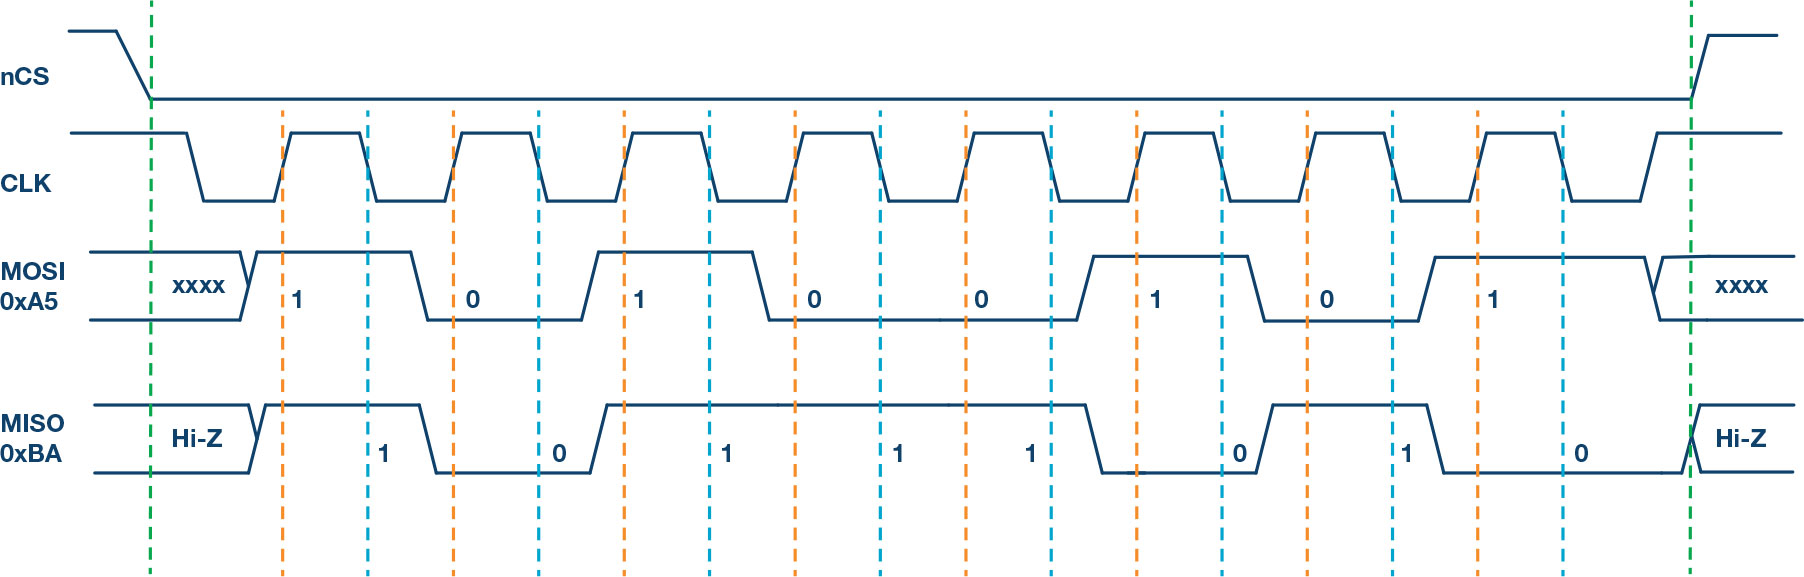
\includegraphics[width=\textwidth]{appendices/digital_communication/spi_protocol.jpg}
\end{figure}

\chapter{Gyroscope Coriolis Effect Proof} \labchap{gyroscope_proof}

The position of the center of mass in the gyroscope body  frame is given by:

\begin{equation}
    B_c = 
    \begin{bmatrix}
        x \\
        y 
    \end{bmatrix}
\end{equation}

The inertial velocity of the mass is given by the positional derivative and the tangential velocity due to rotation:

\begin{equation}
    \dot{B_c} = 
    \begin{bmatrix}
        \dot{x} \\ 
        \dot{y}
    \end{bmatrix}
    + B_\omega \times B_r =
    \begin{bmatrix}
        \dot{x} - \omega y \\
        \dot{y} + \omega x
    \end{bmatrix}
\end{equation}

The inertial acceleration is the next derivative given by:

\begin{equation}
    \ddot{B_c} = 
    \begin{bmatrix}
        \ddot{x} \\
        \ddot{y}
    \end{bmatrix} = 
    \begin{bmatrix}
        \dot{x}-\omega y \\
        \dot{y} + \omega x
    \end{bmatrix}
    + B_\omega \times B_{\dot{r}} = 
    \begin{bmatrix}
        \ddot{x} - 2\omega\dot{y} - \omega^2 x \\
        \ddot{y} + 2\omega\dot{x} - \omega^2 y
    \end{bmatrix}
\end{equation}

The first element in $(3)$ represents the acceleration experienced by the x-axis (driven axis). This axis is actively controlled by the gyroscope driving circuit. The second element is that of the sensing axis (y-axis). Recall Newton’s Second Law of Motion, $F=ma$:

\begin{equation}
    F_y=mB_{\ddot{c}, y} = m(\ddot{y}+2\omega\dot{x}-\omega^2y)
\end{equation}

If the mass starts at the resting position, $y=\dot{y}=\ddot{y}=0$. Therefore, we get:

\begin{equation}
    F_y=2m\omega\dot{x}
\end{equation}

Since the mass is displaced along the x-axis at a high frequency and short distance, $\dot{x}$ is significant and the Coriolis effect generates a high amplitude, proportional displacement in the y-axis. The tuning fork configuration essentially doubles the displacement and makes capacitive detection easier. Additionally, when undergoing linear acceleration, the masses move equally, minimizing sensitivity to shock, vibration, and tilt.
\chapter{Rotation Matrices} \labchap{rotation_matrix}
A rotation matrix is a mathematic model for translating one body's inertial reference frame to another, e.g. local frame to a global frame.
These are used for Eulerian transformations of vectors (i.e. using roll, pitch, and yaw).
To begin deriving these matrices, let's start with a two dimensional rotation matrix:

\begin{equation*}
    R(\theta) = \left[
        \begin{matrix}
            \cos\theta & -\sin\theta \\
            \sin\theta & cos\theta
        \end{matrix}\right]
\end{equation*}

If we rotate a vector, $\vec{v} = \langle x, y \rangle$ with a magnitude, $r$ by $\theta$ degrees about the Z-axis (as shown in Figure \ref{fig:2d_rot}), it will arrive at a new coordinate $\langle x^{\prime}, y^{\prime}\rangle$. 
We can express $\vec{v}$ in polar form as:

\begin{align}
    x &= r\cos\phi \\
    y &= r\sin\phi
\end{align}

Similarly, the rotated vector, $\vec{v}^{\prime}$ in polar form is expressed as:

\begin{align*}
    x^{\prime} &= r\cos(\phi+\theta) \\
    y^{\prime} &= r\sin(\phi+\theta)
\end{align*}

\begin{figure}[h!]
    \caption{2 dimensional rotation of a vector, $A$, to a new set of coordinates, $A'$.}
    \labfig{2d_rot}
    \centering
    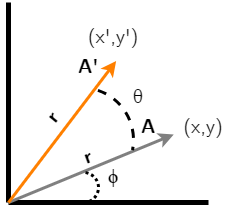
\includegraphics[height=2.5in]{appendices/rotation_matrix/2d_rotation_plot.png}
\end{figure}

Expanding and using trigonometric identities:

\begin{align*}
    x^{\prime} &= r(\cos\phi\cos\theta + \sin\phi\sin\theta) \\
               &= r\cos\phi\cos\theta + r\sin\phi\sin\theta \\
               &= x\cos\theta + y\sin\theta \\
    y^{\prime} &= r(\sin\phi\sin\theta + \cos\phi\sin\theta) \\
               &= r\sin\phi\cos\theta + r\cos\phi\sin\theta \\
               &= y\cos\theta + x\sin\theta
\end{align*}

We can then express the resultant equations in the form of a $2 \times 2$ rotation matrix, $R$, yielding:

\begin{equation*}
    \left[
        \begin{matrix}
            x^{\prime} \\ 
            y^{\prime}
        \end{matrix}
    \right]
    =
    \left[
        \begin{matrix}
            \cos\theta & -\sin\theta \\
            \sin\theta & \cos\theta
        \end{matrix}
    \right]
    \left[
        \begin{matrix}
            x \\
            y
        \end{matrix}
    \right]
    = R(\theta)
    \left[
        \begin{matrix}
            x \\
            y
        \end{matrix}
    \right]
\end{equation*}

\paragraph*{Example} If we have a vessel moving in the a direction at some velocity and it encounters a current, $\vec{v}$ coming in from the starboard quarter, what is the current's influence on the vessel?

\begin{figure}[h!]
    \caption{A vessel encounters a current (orange), $\pmb{v}$, from the forward starboard quarter.}
    \labfig{boat_current}
    \centering
    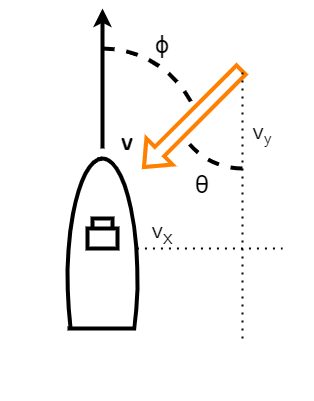
\includegraphics[height=2.5in]{appendices/rotation_matrix/boat_current.png}
\end{figure}

First, we can use the parallel axis theorem to determine that the current is impinging on the vessel at an angle, $\theta$, relative to its longitudinal (y) axis.
We can consider the current vector to be in the global frame and to find its influence on the vessel, we must rotate it to the vessel's local frame and get the resultant vector, $[v_x, v_y]$.
Using a rotation matrix, we can determine that:

\begin{equation*}
    \left[
        \begin{matrix}
            v_x^{\prime} \\
            v_y^{\prime}
        \end{matrix}
    \right] = 
    R(\theta) \left[
        \begin{matrix}
            v_E \\
            v_N
        \end{matrix}
    \right]
\end{equation*}

\section{Three Dimensional Rotation Matrix} \labsec{3d_rot_mat}
In three dimensional space, rotation can be performed about the X-, Y-, or Z-axis. A basic rotation that occurs around a single axis is defined as an "elementary rotation" and given by the following rotation matrices:

\begin{align*}
    R_x(\phi) &= \left[
        \begin{matrix}
            1 & 0 & 0 \\
            0 & \cos\phi & -\sin\phi \\
            0 & \sin\phi & \cos\phi
        \end{matrix}
    \right] \\
    R_y(\theta) &= \left[
        \begin{matrix}
            \cos\theta & 0 & \sin\theta \\
            0 & 1 & 0 \\
            -\sin\theta & 0 & \cos\theta
        \end{matrix}
    \right] \\
    R_z(\psi) &= \left[
        \begin{matrix}
            \cos\psi & -\sin\psi & 0 \\
            \sin\psi & \cos\psi & 0 \\
            0 & 0 & 1
        \end{matrix}
    \right]
\end{align*}

To rotate a three dimensional vector from one frame to another, we must select the order of the axes to be rotated about, then multiply the rotation matrices and vector together.
\paragraph*{Example} What are the components of gravitational acceleration, $a_G$ that affect an airplane in flight at some arbitrary roll ($\phi$), pitch ($\theta$), and yaw ($\psi$)?

\begin{figure}[h!]
    \caption{A plane rotated at some arbitrary roll (red), $\phi$, pitch (blue), $\theta$, and yaw (green), $\psi$, experiences gravitational acceleration in all three axes.}
    \labfig{airplane_rotation}
    \centering
    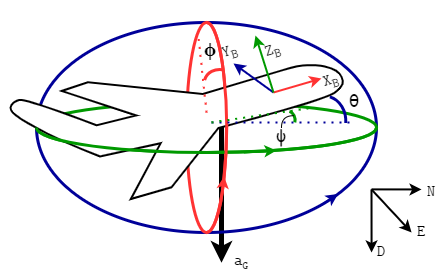
\includegraphics[height=2.5in]{appendices/rotation_matrix/airplane_rotation.png}
\end{figure}

First, we define the gravitational acceleration vector as existing in the global North-East-Down (NED) reference frame, $a_G = \langle a_N, a_E, a_D \rangle = \langle 0, 0, 1 \rangle$.
We will also assume that all of the rotations of the plane are relative to the same NED frame.
We can then perform a yaw-pitch-roll rotation of $a_G$ to get the gravitational acceleration in terms of the plane's coordinate frame, ${}^G_B a$:

\begin{align*}
    {}^G_B a &= R_z(\psi) R_y(\theta) R_x(\phi) a_G \\
    &= 
    \left[
        \begin{matrix}
            \cos\psi & -\sin\psi & 0 \\
            \sin\psi & \cos\psi & 0 \\
            0 & 0 & 1
        \end{matrix}
    \right]
    \left[
        \begin{matrix}
            \cos\theta & 0 & \sin\theta \\
            0 & 1 & 0 \\
            -\sin\theta & 0 & \cos\theta
        \end{matrix}
    \right]
    \left[
        \begin{matrix}
            1 & 0 & 0 \\
            0 & \cos\phi & -\sin\phi \\
            0 & \sin\phi & \cos\phi 
        \end{matrix}
    \right] 
    \left[
        \begin{matrix}
            0 \\
            0 \\
            1
        \end{matrix}
    \right]\\
    {}^G_B a &= 
    \left[
        \begin{matrix}
            \cos\psi\cos\theta & \cos\psi\sin\theta\sin\phi-\sin\psi\cos\theta & \cos\psi\sin\theta\cos\phi+\sin\psi\sin\phi \\
            \sin\psi\cos\theta & \sin\psi\sin\theta\sin\phi+\cos\psi\cos\phi & \sin\psi\sin\theta\cos\phi-\cos\psi\sin\phi \\
            -\sin\theta & \cos\theta\sin\phi & \cos\theta\cos\phi
        \end{matrix}
    \right]
    \left[
        \begin{matrix}
            0 \\
            0 \\
            1
        \end{matrix}
    \right]
\end{align*}
\chapter{Kalman Filter} \labchap{kalman_filter}

\section{Introduction} 
The Kalman Filter is a recursive algorithm introduced in the 1960's as a method to track, estimate, and predict the state of a system and corresponding uncertainties \cite{Kalman:1960}.
This filter integrates a dynamic (linear) model of the system, control inputs, measurements, and biases/uncertainties into a single algorithm.
This effectively fuses together system inputs and responses and extrapolates what the system is currently doing and expected to do.
One key advantage of this algorithm is that it only requires the guess of the previous state to estimate the current state. 
This massively decreases the memory and processing costs as the history of inputs, measurements, and uncertainties does not need to be remembered or analyzed.
However, it does have some limitations when the sensor data is noisy or the control inputs cannot be linearly mapped to the system state.
Random errors in the sensor data may cause the filter to behave unpredictably and non-linearity prevents proper fusion entirely.
This problem can be solved using an Extended Kalman Filter, but that is out of scope for now.

\section{Kalman Filter in One Dimension}
The uni-dimensional Kalman filter is a special, idealized case for the Kalman filter.
It is more convenient as a teaching tool as it does not include the complex matrix and vector operations the general multi-dimensional Kalman filter requires.
However, this only makes this type useful for tracking and estimating a single variable.

Multiple uni-dimensional Kalman filters can be run in parallel or chained together to mimic a multi-dimensional filter, however, this will unnecessarily increase the computational resources required for the calculations and will reduce the quality of the filtering overall.

\subsection{The Kalman Gain} 
In a Kalman filter, the Kalman Gain, denoted as $K_n$, is calculated at each iteration of the filter.
The Kalman gain is bounded by: $0 <= Kn <= 1$ and prioritizes predictions of the system state from the estimation or the measurement, based on related uncertainties\footnote{\textbf{Important note:} When measurement uncertainty is very large, and the estimate uncertainty is small, $K_n << 1$, hence big weight to the estimate and small weight to the measurement. When the opposite is true, $K_n -> 1$, meaning a large weight to the measurement and a small weight to the estimate. This is how the Kalman filter can regulate and smooth out noisy data by knowing the uncertainties.}.

\begin{equation} \labeq{kalman_gain}
    \begin{aligned}
        K_n &= \frac{\text{Estimate Uncertainty}}{\text{Estimate Uncertainty + Measurement Uncertainty}} \\
            &= \frac{p_{n,n-1}}{p_{n,n-1} + r_n}
    \end{aligned}
\end{equation}

We can then define the State Update Equation for a system where $\hat{x}$ is the predicted state and $z$ is the measured state:

\begin{equation} \labeq{kalman_state_update}
    \begin{aligned}
        \hat{x}_{n,n} &= \hat{x}_{n,n-1} + K_n(z_n - \hat{x}_{n,n-1}) \\
                        &= (1-K_n)\hat{x}_{n,n-1} + K_n z_n \\
    \end{aligned}
\end{equation}

\subsection{The Estimate Uncertainty Update Equation} 
The estimate uncertainty or covariance update equation predicts the uncertainty associated with the current estimate.
The estimate uncertainty should approach (converge) to 0 with each filter iteration as the filter improves its guessing accuracy.
However, if the measurement uncertainty is large ($K_n << 1$), the estimate uncertainty will converge more slowly.
The opposite is true if the measurement uncertainty is small.
Basically, the more precise your measurements are, the faster the Kalman filter will converge on the best estimate.

\begin{gather}
    p_{n,n} = (1-K_n)p_{n,n-1} \\
    \begin{aligned}
        \text{where } &p_{n,n} \text{ is the estimate uncertainty at the current state} \\
                        &K_n \text{ is the Kalman gain at the current state} \\
                        &p_{n,n-1} \text{ is the estimate uncertainty of the previous state}
    \end{aligned} \notag
\end{gather}

\subsection{The Estimate Uncertainty Extrapolation Equation} 
Another Kalman equation is how the filter predicts future uncertainties and is called the Estimate Uncertainty Extrapolation Equation or the Estimate Covariance Extrapolation Equation.
Like with the State Extrapolation Equations, this is done with dynamic models and will be unique to every example.
FOr a moving vehicle, one example might be:

\begin{gather} \labeq{covariance_extrapolation}
    p_{n+1,n}^x = p_{n,n}^x + \Delta t p_{n,n}^{\dot{x}} \\
    p_{n+1,n}^{\dot{x}} = p_{n,n}^{\dot{x}} \\
    \begin{aligned}
    \text{where } &x \text{ is the vehicle displacement, and} \\
                  &\dot{x} \text{ is the vehicle velocity}
    \end{aligned}
\end{gather}

\subsection{Putting it all Together}
First, the filter is initialized with a first guess ($\hat{x}_{0,0}$) and an associated uncertainty ($p_{0,0}$).
These values are passed into the dynamic model equations and Equation \ref{eq:covariance_extrapolation} to predict the state at the first measurement ($x_{1,0}$) and the associated uncertainty ($p_{1,0}$).
This is shown as Step 0 in Figure \ref{fig:kalman_filter_process}.
Then, we can take a measurement ($z_n$) and record its uncertainty ($r_n$), using the latter to determine the Kalman gain with Equation \ref{eq:kalman_gain}.
We can then estimate the current state value using Equation \ref{eq:kalman_state_update} using the recorded measurement and the Kalman gain ($K_n$).
The current state estimate and its uncertainty can then be outputted from the filter and used in applications; this process is shown as Steps 1, 2a, and 2b in the figure below.
These values are then fed into the dynamic model to predict the next state and estimate the associated uncertainty (Step 3 in the below diagram).
Optionally, these predicted values can be outputted from the model as well, as the application requires.
This process repeats for every measurement with $n$ incrementing every time.

\begin{figure}[h!]
    \includegraphics[width=\textwidth]{appendices/kalman-filter/KalmanFilter.png}
    \caption[Kalman Filter Diagram]{Process diagram for a Kalman filter.}
    \labfig{kalman_filter_process}
\end{figure}

\begin{fitbox}[frametitle=Example]
    In this example, we will be estimating the depth of an ROV using a 1D Kalman filter.
    We will be assuming the ROV depth remains constant and its location in space does not matter or change.
    For example's sake, we shall know for an absolute fact that the ROV is at a depth of 50-meters ($x=50 \text{ m}$).
    We will also assume that our depth sensor has a standard deviation of 5-meters ($\sigma=5 \text{ m}$), therefore we will have a measurement variance or uncertainty of 25-meters ($r=25 \text{ m}^2$)

    \paragraph*{Iteration 0}
    \begin{equation*}
        \begin{aligned}
            0 &: \text{Estimate depth: } \hat{x}_{0,0} = \textbf{60 m} \\
                &: \text{Estimate uncertainty: } p_{0,0} = \textbf{225 m}^2 \\
            3 &: \text{Predicted depth: } \hat{x}_{1,0} = \hat{x}_{0,0} = \textbf{60 m} \\
                &: \text{Prediction uncertainty: } p_{1,0} = p_{0,0} = \textbf{225 m}^2 \\
        \end{aligned}
    \end{equation*}

    \paragraph*{Iteration 1}
    \begin{equation*}
        \begin{aligned}
            1 &: \text{Measure depth: } z_1 = \textbf{48.54 m} \\
                &: \text{Measurement uncertainty: } r_1 = \textbf{25 m}^2 \\
            2 &: \text{Kalman gain } K_1 = \frac{p_{1,0}}{p_{1,0}+r_1} = \frac{255}{255 + 25} = \textbf{0.9} \\
                &: \text{Estimated depth: } \hat{x}_{1,1} = \hat{x}_{1,0} + K_1(z_1 - \hat{x}_{1,0}) = 60 + 0.9(48.54-60) = \textbf{49.69 m} \\
                &: \text{Estimate uncertainty: } p_{1,1} = (1-K_1)p_{1,0} = (1-0.9)225 = \textbf{22.5 m}^2 \\
            3 &: \text{Predicted depth: } \hat{x}_{2,1} = \hat{x}_{1,1} = \textbf{49.69 m} \\
                &: \text{Prediction uncertainty: } p_{1,0} = p_{1,1} = \textbf{22.5 m}^2 \\
        \end{aligned}
    \end{equation*}

    \paragraph*{Iteration 2}
    \begin{equation*}
        \begin{aligned}
            1 &: \text{Measure depth: } z_2 = \textbf{47.11 m} \\
                &: \text{Measurement uncertainty: } r_2 = \textbf{25 m}^2 \\
            2 &: \text{Kalman gain } K_2 = \frac{p_{2,1}}{p_{2,1}+r_2} = \frac{22.5}{22.5 + 25} = \textbf{0.47} \\
                &: \text{Estimated depth: } \hat{x}_{2,2} = \hat{x}_{2,1} + K_2(z_2 - \hat{x}_{2,1}) = 49.69 + 0.47(47.11-49.69) = \textbf{48.47 m} \\
                &: \text{Estimate uncertainty: } p_{2,2} = (1-K_2)p_{2,1} = (1-0.47)22.5 = \textbf{11.84 m}^2 \\
            3 &: \text{Predicted depth: } \hat{x}_{3,2} = \hat{x}_{2,2} = \textbf{48.47 m} \\
                &: \text{Prediction uncertainty: } p_{3,2} = p_{2,2} = \textbf{11.84 m}^2 \\
        \end{aligned}
    \end{equation*}

    \begin{center}
        \begin{tabular}{c | c | c | c | c | c | c | c}
        \toprule
        & \multicolumn{2}{c}{Measurements} & \multicolumn{3}{c}{Current Estimates} & \multicolumn{2}{c}{Predictions} \\
        \midrule
        n & $z_n$ & $r_n$ & $K_n$ & $\hat{x}_{n,n}$ & $ p_{n,n} $ & $ \hat{x}_{n+1,n}$ & $ p_{n+1,n} $ \\
        \midrule

        0  & ---  & -- & ---  & 60.0 & 225  & 60.0 & 225  \\
        1  & 48.5 & 25 & 0.90 & 49.7 & 22.5 & 49.7 & 22.5 \\
        2  & 47.1 & 25 & 0.47 & 48.4 & 11.8 & 48.4 & 11.8 \\
        3  & 55.0 & 25 & 0.32 & 50.6 & 8.03 & 50.6 & 8.03 \\
        4  & 55.2 & 25 & 0.24 & 51.7 & 6.08 & 51.7 & 6.08 \\
        5  & 49.9 & 25 & 0.20 & 51.3 & 4.89 & 51.3 & 4.89 \\
        6  & 40.6 & 25 & 0.16 & 49.6 & 4.09 & 49.6 & 4.09 \\
        7  & 46.7 & 25 & 0.14 & 49.2 & 3.52 & 49.2 & 3.52 \\
        8  & 50.1 & 25 & 0.12 & 49.3 & 3.08 & 49.3 & 3.08 \\
        9  & 51.3 & 25 & 0.11 & 49.5 & 2.74 & 49.5 & 2.74 \\
        10 & 50.0 & 25 & 0.10 & 49.6 & 2.47 & 49.6 & 2.47 \\

        \bottomrule
        \end{tabular}
    \end{center}

    \begin{center}
        \includegraphics[height=3in]{appendices/kalman-filter/1D_kalman_filter_results.png}
    \end{center}

    We can see from the figure that the Kalman filter eventually converges on the true value and considerably smoothes out the noisy measurements.
    The error bars on the estimate plot (blue) also show that the Kalman filter increases its confidence with every iteration as it converges to the true value.
    The oscillation shown in the estimates are a result of the gains being slightly off from their ideal value.
    Tuning the process noise variable (q) can cause the filter to converge quickly and confidently to the true value in fewer iterations.

\end{fitbox}

\subsection{Process Noise} In the real world, there are uncertainties in the system's dynamic model.
Uncertainty is caused by unanticipated changes in the system due to external factors.
This can be drift caused by ocean current, wind blowing a rocket to the side, drag, friction, even time dilation in extreme cases.
Generally, these uncertainties can be combined into the Process Noise gain denoted by $q$.
To account for process noise, it must be included in the Covariance Extrapolation Equation (Equation \ref{eq:covariance_extrapolation}).

If the model is not known to be good or is very noisy, we can increase the process noise gain to reduce the lag error.

\begin{equation}
    p_{n+1,n} = p_{n,n} + q
\end{equation}

\subsection*{Further Reading}
The book \textit{Kalman Filter: From the Ground Up} \cite{Becker:2023} provides an excellent resource on the intuitive understanding of the Kalman Filter and some of its more advanced applications like multi-variate Kalman Filters, Extended Kalman Filters, and applying Kalman Filters in sensor fusion applications.
\chapter{Traceability Matrix} \label{chap:traceability_matrix}
A traceability matrix is an artifact within Systems Engineering that tracks the stakeholder requirements, capabilities, system requirements, and testing methodologies.
The primary purpose is to give a Lead Systems Engineer other other team member quick access to all of the driving information for the product and trace the requirement lifecycle.
Each matrix has eight columns that contain information about the requirement:

\paragraph*{ID} This is the identification number for the requirement.
Stakeholder requirements will start with the prefix: "SR".
Capabilities will be triple-digit numbers with 100-level being "threshold", 200-level being "reach", and 300-level being "stretch" capabilities.
Component-level requirements will be divided into sections and subsections in the format "X.X.X.X" depending on the section and depth of the requirement.
For example, the first requirement in the first section, first subsection of the component-level matrix will have the ID "1.1.1".

\paragraph*{Description} Each requirement and capability needs to have a brief, single sentence description that details the feature.
The description should follow the guidelines laid out by NASA\footnote{\url{https://www.nasa.gov/seh/appendix-c-how-to-write-a-good-requirement}}.
They should be unambiguous, testable, verifiable, and consistent in both terminology and can either be functional or non-functional.
Functional requirements directly drive a feature of the product, whereas a non-functional requirement drives an aesthetic or interface choice.

\paragraph*{Weight} The requirements and capabilities should all have a weight associated with them.
These can be based on stakeholder preferences, developer capabilities, technology limitations, etc.
The weight is a number greater than 0, but less than 1 and typically only expressed as a single decimal.

\paragraph*{Priority} Derived from the weight, the priority is the relative importance of a particular requirement or capability to others.
It is calculated using Equation \ref{eq:priority}. 
A higher priority means a requirement is more important to implement on the product.
For capabilities, the priority is calculated slightly differently.
The weight of a capability is compared to all of the other weights in the same category and the one(s) beneath it.
For instance, a threshold capability's priority will only factor in the weights of other threshold capabilities.
But, a stretch capability's priority will factor in the weights of all capabilities in the design.

\begin{equation} \label{eq:priority}
    P = \frac{w_c}{\sum w} \times 100
\end{equation}

\paragraph*{Owner} The person who is responsible for a requirement or capability is called the owner.
This individual is in charge of developing, implementing, verifying, testing, and validating the product feature.
They do not have to be the only person working on that feature, but they are responsible for it.
This individual should also be the one tracking and updating the requirement or capability status throughout the traceability matrix. 

\paragraph*{Verified?} The verification of a requirement or capability requires an inspection to ensure that it is present.
Component-level requirements will have a test number that should also be tracked in the traceability artifact to describe what test was performed that verified the requirement.
Until a requirement or capability is successfully inspected, the answer to the column header is, "No", but can be changed to "Yes" once verified.
A requirement can be subject to a variety of methods to verify it is implemented:

{
\renewcommand{\descriptionlabel}[1]{\hspace{\labelsep}\textbf{#1}}
\begin{description}
    \item[Inspection:] The nondestructive examination of a product or system using one or more of the five senses (visual, auditory, olfactory, tactile, taste). 
    It may also include simple physical manipulation and measurements.
    
    \item[Demonstration:] The manipulation of the product or system as it is intended to be used to verify that the results are as planned or expected.								
    
    \item[Test:] The verification of a product or system using a controlled and predefined series of inputs, data, or stimuli to ensure that the product or system will produce a very specific and predefined output as specified by the requirements.								
    
    \item[Analysis:] The verification of a product or system using models, calculations and testing equipment.
    Analysis allows someone to make predictive statements about the typical performance of a product or system based on the confirmed test results of a sample set or by combining the outcome of individual tests to conclude something new about the product or system.
    It is often used to predict the breaking point or failure of a product or system by using nondestructive tests to extrapolate the failure point.
\end{description}
}

\paragraph*{Validated?} Validation of a capability or requirement occurs when the feature is fully integrated to the system and tested.
It is not enough that it is present, rather it must also contribute to the system as designed without impinging on another feature.
This is another "Yes"/"No" column depending on if the feature has been fully integrated to the system.

\paragraph*{Status} The last major column to consider in the matrix is the status column.
This lets the reader know if the capability or requirement has been reviewed or rejected, is undergoing testing, delivered, etc.
The value of this column is pulled from Table \ref{tab:req_status} based on the requirement's stage in the lifecycle (see Figure \ref{fig:requirement_lifecycle}).

\begin{table}
    % \setlength{\arrayrulewidth}{0.5mm}
    % \setlength{\tabcolsep}{18pt}
    \renewcommand{\arraystretch}{1.5}
    \centering
    \caption{Description of requirement statuses}
    \begin{tabular}{|c | p{0.225\textwidth} || p{0.7\textwidth}|}
        \hline
        UR  & Under Review          & Requirement has been submitted and is under review \\
        A   & Accepted              & Requirement has been reviewed and accepted into the artifact \\
        R   & Rejected              & Requirement has been reviewed and rejected from the artifact \\
        TIP & Testing in Progress   & Requirement is currently being tested \\
        TS  & Test Successful       & Requirement has been successfully tested, but not yet delivered \\
        TF  & Test Failure          & Requirement failed testing and needs further development \\
        D   & Delivered             & Requirement has been fully realized and delivered \\
        \hline
    \end{tabular}
    \label{tab:req_status}
\end{table}

\section{Requirement Lifecylce}
Requirements are initially created at the start of the project and are expected to be monitored and have their status updated as the project continues.
Once a requirement is written, it is up the Lead Systems Engineer, or other team members, to review the requirement and determine if it is suitible for the project.
The major considerations are 1) "is the requirement relevant?", 2) "is the requirement unambiguous?", 3) "is the requirement testable?", and 4) "is the requirement complete?"
If the requirement does not meet any of these criteria, it can be rejected for re-writing by its owner.
Once the requirement is accepted, development for it can begin.
It is up to the owner to ensure that the feature detailed by the requirement is properly designed and integrated into the larger system.
When the owner verifies the feature and is ready to validate it with the system, they can begin the testing process ad update the status to "TIP" in the traceability matrix.
If the test was successful, the requirement status should reflect this; same for a test failure.
If the validation fails, the requirement may need to be re-written or re-tested in a different system configuration.
Finally, when the feature is fully integrated with the product and released, the status can be set to "delivered" and the feature can be considered fully completed.

\begin{figure}
    \centering
    \caption{Lifecycle of a requirement}
    \includegraphics[height=6in]{appendices/traceability-matrix/requirement_lifecycle.png}
    \label{fig:requirement_lifecycle}
\end{figure}

\chapter{Wave Estimating Algorithm for Vessels Experiment (WEAVE)} \label{chap:weave}

\section{Introduction} \label{sec:weave_intro}

As a buoy is floats on top of waves, it experiences an acceleration proportional to the hydrodynamic forces exerted on it by $\pmb{F} = m\pmb{a}$. 
As a result, the buoy is displaced by a measurable amount as a wave passes through it. 
A wave buoy uses an accelerometer to measure the vertical acceleration component of this motion. 
By double integrating the signal with respect to time via the following equation, we can get the vertical displacement $z(t)$.

\begin{equation}
    z(t) = \frac{1}{2} a_z(t) \Delta t^2 + e
\end{equation}

Where $a_z(t)$ is the vertical acceleration time series, $\Delta t$ is the time since the last value update, and $e$ is the measurement error introduced by the sensor errors and integration errors (more on this later).

The equation shows that the error is multiplied over time, causing the reading to drift. 
Industry standard buoys like the [DataWell WaveRider 4](https://datawell.nl/products/directional-waverider-4/) use high precision, regularly-calibrated sensors to minimize and account for the measurement error.

These types of uni-axial measurement buoys also rely on the measurement axis always being parallel to the Earth vertical axis. 
While the WaveRider 4 buoy accomplishes this by suspending the accelerometer on a platform in a fluid specifically tuned to act as a massive dampener, this comes at an increase to size and cost. 
Additionally, should this platform become misaligned to the global vertical axis, the measurements will always be of a component of the vertical acceleration and therefore introduce a bias in the calculations.

In this document, a procedure to use body frame coordinate rotation will be introduced that will eliminate the error and bias of a misaligned vertical axis measurement. 
The procedure will be implemented in two different ways: 1) a spectral analysis using the procedure laid out in Longuet-Higgins, 1963 and used by the WaveRider 4 buoy, 2) a novel oscillatory motion analysis based upon the work of Madgwick, 2013 that provides an instantaneous estimate of the wave height and direction.

\section{Background}
Inertial Measurement Units (IMUs) consist of an array of sensors that measure inertial forces acting on a body. 
Each measurement axis of the IMU is referred to as a degree of freedom (DOF). 
Advanced IMUs utilize 9 DOFs of measurements and also called Magnetic, Angular Rate, and Gravity (MARG) arrays. 
These sensors use a tri-axial magnetometer, gyroscope, and accelerometer, respectively to determine a body’s pose or orientation in 3D space, relative to a magnetic and gravitational field.

Using sensor fusion algorithms, it is possible to fuse the MARG array data into a unified representation of the body pose called the Attitude and Heading Reference System (AHRS). 
There are several such algorithms, most notably the complementary filter, the Kalman Filter, the Mahony filter, and the Madgwick filter. 
Madgwick’s filter is ideal for embedded applications because of its high accuracy, low performance cost, and ability to incorporate gyroscopic and magnetic drift compensation during runtime. 
This makes the attitude estimate over accurate over time and across a larger range of body motions. 
Therefore, this algorithm will be used exclusively during this study for sensor fusion.

\subsection{Quaternion Representation}

The crux of Madgwick’s filter is a gradient descent estimation of the body quaternion. 
The quaternion is a 4-dimensional representation of orientation that is free from infinite discontinuities found in 3-dimensional counterpart, Euler angles. 
The quaternion represents a 3D coordinate frame’s rotation about a unit vector in the base coordinate frame. 
his is represented graphically in the Figure \ref{fig:weave_frame_rot} where the mutually orthogonal axes, $A_x$, $A_y$, $A_z$, $B_x$, $B_y$, $B_z$ represent the 3D frames $A$ and $B$, respectively.
When frame $B$ is rotated by some angle, $\theta$, about the unit vector, ${}^A \pmb{r}$, it now has an orientation relative to frame $A$ that can be expressed as the quaternion:

\begin{equation}
    {}^A_B\textbf{q} = \begin{bmatrix} q_1 & q_2 & q_3 & q_4 \end{bmatrix} = \begin{bmatrix} \cos\frac{\theta}{2} & -r_x\sin\frac{\theta}{2} & -r_y\sin\frac{\theta}{2} & -r_z\sin\frac{\theta}{2} \end{bmatrix}
\end{equation}

Note that we adopt the notation introduced by Craig, 2005. 
The preceding superscript denotes the ``base'' or ``from'' coordinate frame and the preceding subscript denotes the ``derived'' or ``to'' coordinate frame. 
In the previous example, ${}_B^Aq$ is the quaternion representing the rotation \textit{from} frame $A$ \textit{to} frame $B$.

\subsection{Quaternion Application to Rotations}

If, by convention, we assume all bodies that are not Earth have some rotation relative to Earth’s central coordinate frame, then we can represent any body’s orientation as ${}^B_G\pmb{q}$ where $G$ is the global frame and $B$ is the body frame. 
If we also assume that the body is within Earth’s gravitational and magnetic field, then we can use a MARG array to determine ${}^B_G\pmb{q}$ via Madgwick’s filter.

Since quaternions represent coordinate frame rotations, we can use them to rotate 3D vectors from one frame to another. 
For example, in any given orientation in Earth’s gravitational field, there will always be components of gravitational acceleration within a body frame’s acceleration. 
Therefore, an accelerometer in the body frame will always be measuring the gravitational acceleration vector, ${}^G\pmb{a}$, and the body acceleration vector, ${}^B\pmb{a}$. 
If we want to eliminate the gravitational signal, we can rotation the gravitational acceleration vector from the global coordinate frame to the body frame and subtract it from our readings. 
This will yield the body linear accelerations, ${}^B\pmb{a}_l$, defined as:

\begin{gather}
    {}^G_B\pmb{a} = {}^G_B\pmb{q} \cdot {}^G\pmb{a} \cdot {}^G_B\pmb{q}^{-1} \\
    {}^B\pmb{a}_l = {}^B\pmb{a} - {}^G_B\pmb{a}
\end{gather}

Again, using the notation from Craig, 2005 to denote the ``from'' and ``to'' frames, respectively. Also note that ${}^G_B\pmb{q}^{-1}$ is the inverse quaternion as defined by:

\begin{equation*}
    {}^G_B\pmb{q}^{-1} = \begin{bmatrix} -q_1 & -q_2 & -q_3 & -q_4 \end{bmatrix}
\end{equation*}

Alternatively, we can rotate the body accelerations to the global frame and get global linear accelerations, ${}^B_G\pmb{a}_l$, via a similar operation:

\begin{gather}
    {}^B_G\pmb{a} = {}^B_G\pmb{q} \cdot {}^B\pmb{a} \cdot {}^B_G\pmb{q}^{-1} \\
    {}^B_G\pmb{a}_l = {}^B_G\pmb{a} - {}^G\pmb{a}
\end{gather}

By convention, the global coordinate frame is typically referred to as North-East-Down (NED) and therefore, ${}^G\pmb{a} = \begin{bmatrix} 0 & 0 & 1 \end{bmatrix}$

\section{Spectral Analysis Theory}

For the spectral analysis, the work by Longuet-Higgins, 1963 will be heavily utilized. 
The displacement vector should be subsampled to 2.56 Hz. 
Over a 200-second interval, a total of $N=512$ samples are collected. 
We can then obtain a frequency spectrum via the Fast Fourier Transform (FFT). 
The spectrum will have a range of $0$ to $\frac{f_s}{2}=1.28 \text{Hz}$ and a resolution of $\frac{f_s}{N}=0.005 \text{Hz}$.
The FFT yields Fourier coefficients via:

\begin{equation}
    \sum_{k=0}^{N-1} w_k h_k e^{\frac{2\pi kl}{N}}
\end{equation}

Where $f_l=\frac{1}{N\Delta t}$ and $= 0 \ldots N-1$ and the $w_k$ element is a windowing function. 
Datawell uses a Hann windowing function which attenuates signals in the higher frequency domains:

\begin{equation}
    w_k = \frac{1}{2} [1-\cos{\frac{2\pi k}{N}}] \text{ where } k=0 \ldots N-1
\end{equation}

We can normalize these coefficients via:

\begin{equation}
    w_{norm} = \sqrt{f_s \sum_{k=0}^{N-1}w_k^2}
\end{equation}

Since we have time series data for all three axes, we can take the spectra for each series. Each series contains a vector of coefficients and can be expressed in vector notation as:

\begin{align}
    a_N &= \alpha_N + i\beta_N \\
    a_E &= \alpha_E + i\beta_E \\
    a_D &= \alpha_D + i\beta_D
\end{align}

We can then define the co-spectra ($C$) and the quad-spectra ($Q$) as follows:

\begin{gather}
    C_{xy} = a_x \cdot a_y = \alpha_x \alpha_y + \beta_x \beta_y \\
    C_{xy} = a_x \times a_y = \alpha_x \beta_y - \beta_x \alpha_y
\end{gather}

Then, we can arrange them into 3 by 3 matrices to obtain the final definition of the acceleration spectra:

\begin{gather}
    \begin{bmatrix}
        C_{NN} & C_{NE} & C_{ND} \\
        C_{EN} & C_{EE} & C_{ED} \\
        C_{DN} & C_{DE} & C_{DD}
    \end{bmatrix} \\
    \begin{bmatrix}
        0 & 0 & Q_{ED} \\
        0 & 0 & Q_{ND} \\
        Q_{DE} & Q_{DN} & 0
    \end{bmatrix}
\end{gather}

Note that by definition, $Q_{NN}=Q{EE}=Q_{DD}=0$ and $Q_EN$ and $Q_NE$ represent eddy currents and are not considered.

These spectra can represent different wave parameters such as wave direction, direction spread, wave ellipticity, and power spectral density (PSD). 
The wave direction, $\theta_0$, is defined as the angle from which the waves are approaching relative to geographic north.

\begin{equation}
    \theta_0 = \arctan{\frac{-Q_{ED}}{Q_{ND}}}
\end{equation}

The direction spread can be more difficultly determined via:

\begin{gather}
    S = \sqrt{2-2m_1} \\
    \begin{aligned}
        \text{where }   &m_1 = \sqrt{a_1^2 + b_1^2} \\
                        &a_1 = \frac{Q_{ND}}{\sqrt{(C_{NN}+C_{EE})C_{DD}}} \\
                        &b_1 = \frac{-Q_{ED}}{\sqrt{(C_{NN}+C_{EE})C_{DD}}}
    \end{aligned}
\end{gather}

The wave ellipticity describes the shape of the wave. 
Specifically, the particle trajectories. 
For wavelengths much smaller than the water depth, the particles will follow a circular trajectory, thus the ellipticity is near 1. 
However, as the wavelength approaches the water depth, the vertical displacements reduce and the ellipticity becomes less than 1, trending towards 0. 
We can determine this parameter via:

\begin{equation}
    \epsilon = \frac{1}{k} = \sqrt{\frac{C_{DD}}{C_{NN}+C_{EE}}}
\end{equation}

Finally, the PSD describes the amount of energy present in the signal across the entire frequency spectrum. 
The PSD for the vertical axis is considered the wave spectrum and is calculated by:

\begin{equation}
    E(f) = C_{DD} = \alpha^2_D + \beta^2_D
\end{equation}

By taking the integral of the PSD we can find the n-th spectral moment of the signal. 
The zeroth spectral moment, $m_0$, can tell us a lot of information such as the significant wave height, $H_s$, and the peak wave period, $T_p$.

\begin{gather}
    m_0 = \int^\infty_0 f^0E(f)df \\
    H_s = 4\sqrt{m_0} = H_{m_0} \\
    T_p = 5 \sqrt{H_s}
\end{gather}

\section{Oscillitory Motion Tracking Theory}

The spectral analysis method is the industry standard and recommended by NOAA in the [NDBC Technical Document 96-01](https://www.ndbc.noaa.gov/wavemeas.pdf). 
However, the spectra needs to be analyzed over time. 
The accuracy of the spectral analysis directly correlates with its sample interval; instantaneous intervals will never be completely representative whereas infinite intervals will be 100\% accurate.
The above methodology offers a balance of accuracy and reporting time. 
But, the sample interval of 200-seconds may be too long for some applications. 
Therefore, in this section we will explore an alternative approach where the wave height is directly computed instantaneously using accelerometer integration and feedback error correction.

We start by using the rotated linear accelerations derived in the Section \ref{sec:weave_intro}. 
These can be integrated over time to get velocity, $\pmb{v}$, as shown below:

\begin{equation}
    {}^G\pmb{v}(t) = {}^G\pmb{a}(t) \Delta t
\end{equation}

The integration error accumulates over time and causes the signal to drift, or deviate from the true value. 
We can consider this drift a velocity signal with infinite period and apply a high-pass filter with an extremely small cutoff frequency to attenuate the error. 
The filter design is discussed in an upcoming subsection. 
We can perform another integration to get the buoy displacement in the global frame:

\begin{equation}
    {}^G\pmb{s}(t) = {}^G\pmb{v}(t)\Delta t + \pmb{e} = {}^G\pmb{a}(t) \Delta t^2 + \pmb{e}
\end{equation}

The integration error for displacement is also fed by the error from velocity, so this value will drift faster over time. 
Again, we can consider the drift an infinite period signal and apply another high-pass filter. 
Madgwick, 2013 shows this method is effective for motions where a zero-velocity point occurs (e.g. at the bottom of a step). 
But, this method needs to be tested on a constantly moving object, like a wave buoy.

\subsection{Filter Design}
The goals of the velocity and displacement filters are to maximize the attenuation of the error signal while minimizing both the attenuation of the desired signal and the induced phase shift. 
The ideal filter will have these criteria, but they are impossible to design. 
Therefore, we must compromise between the two.

There are four main digital infinite impulse response filters: Bessel, Butterworth, Chebyshev (Type I and Type II), and Elliptic. 
Each filter can be expressed by its ``order'' or how many times the filter is applied to the signal. 
The higher the order, the steeper the transition and the closer the magnitude response becomes to ideal. 
But, this often comes at the cost of dramatically increasing phase shift. 
The main filters can generally be ranked in the order given above: from left to right, the transition becomes steeper with a smaller order; from right to left, the phase shift is more linear in the pass band.

If a more linear/minimized phase shift is desired, then a low order Bessel or Butterworth filter is best. 
Though, their transition areas can span many frequency decades. 
Since our cutoff frequency is extremely small, we want the most reactive filter with the narrowest transition. 
To make the Bessel and Butterworth filter fulfill this criterion, we need to substantially increase their orders, eliminating their beneficial phase shift characteristic.

The two remaining filters, Chebyshev and Elliptic, have sharper transition regions but at the cost of non-linear phase shifts and ripple in the pass and stop bands. 
For a bandpass filter design, we can define a couple of parameters: a low-stop frequency of 0.025 Hz, a low-pass frequency of 0.05 Hz, a high-stop frequency of 2.0 Hz, a high-pass frequency of 0.25 Hz, a stop attenuation of 100 dB, and a pass attenuation of 0.1 dB. 
With these values, different bode plots for Chebyshev Type I (Figure \ref{subfig:chebyshev_1}), Chebyshev Type II (Figure \ref{subfig:chebyshev_2}), and Elliptic (Figure \ref{subfig:elliptic}) filters were created.

\begin{figure}[h!]
    \centering
    \subfloat[Chebyshev Type I filter]{\includegraphics[width=0.25\textwidth]{appendices/weave/chebyshev_1.png}\label{subfig:chebyshev_1}}\hskip3ex
    \subfloat[Chebyshev Type II filter]{\includegraphics[width=0.25\textwidth]{appendices/weave/chebyshev_2.png}\label{subfig:chebyshev_2}}\hskip3ex
    \subfloat[Elliptic filter]{\includegraphics[width=0.25\textwidth]{appendices/weave/elliptic.png}\label{subfig:elliptic}}\hskip3ex
    \caption[Digital filter bode plots]{Bode plots for Chebyshev and Elliptical filters using a low-stop frequency of 0.025 Hz, a low-pass freuqnecy of 0.05 Hz, a high-stop frequency of 2.0 Hz, a high-pass frequency of 0.25 Hz, a stop attenuation of 100 dB, and a pass attenuation of 0.1 dB.}
    \labfig{filter_bode_plots}
\end{figure}

From these plots, we can see that the both the Chebyshev Type II and Elliptic filter have undesired ripple on the stop bands and the phase shift is very non-linear. 
The Chebyshev Type I filter on the other hand has a much sharper attenuation of the stop bands without any ripple at the cost of some more phase shift. 
We will therefore be using the Chebyshev Type I filter for our analysis.

\section{Methodology}
The two wave analysis techniques will be performed in post-processing after a data collection period. 
Data will be collected using the Thetis inertial datalogger and the [x-IMU3 datalogger](https://x-io.co.uk/x-imu3/). 
The devices will be rigidly attached to the top of a Datawell WaveRider4 buoy and will be accepted as the ground truth for the experiment and used to validate the spectral analysis procedure.

The devices will be deployed for a total of six hours on five different days since the batteries have to be recharged after that length of deployment. 
Data will be offloaded and stored onto a computer after recovery. 
Both Thetis and the x-IMU3 will supply data at 64 Hz meaning each batch of data contains 1.4 million points for a total of 6.9 million data points. 
Using the Madgwick filter, the data points will be used to compute the buoy orientation and linear acceleration over time.

\subsection{For Spectral Analysis}
The linear acceleration dataset wil be subsampled from 64 Hz to about 2.56 Hz using a rolling average filer of $N=25$ samples. 
This will eliminate most of the high frequency noise while still preserving the wave motion signal. 
From here, the data analysis procedure from the previous section will be used to calculated the wave statistics, averaged over each hour of runtime. 
These can be directly compared to the data pulled from the wave buoy using a Root Mean Square Error ($RMSE$) as shown below:

\begin{equation}
    RMSE_H = \sqrt{\frac{\sum{(H_{sX}-H_{sB})^2}}{N}}
\end{equation}

Where $H_{sX}$ is the significant wave height calculated by the inertial data loggers, $H_{sB}$ is the significant wave height reported by the buoy, and $N$ is the number of samples.

\begin{equation}
    RMSE_T = \sqrt{\frac{\sum{(T_{pX}-T_{pB})^2}}{N}}
\end{equation}

Where $T_{pX}$ is the significant wave height calculated by the inertial data loggers, $T_{pB}$ is the significant wave height reported by the buoy, and $N$ is the number of samples.

Note that due to the limited sample time, the comparisons are only valid for a small wave regime. 
The results section will detail the validity more in-depth, but for a more accurate analysis, these instruments must be deployed for longer under a wider array of waves.

\subsection{For the Oscillatory Motion Tracking Analysis}

The data will again be subsampled to about 4 Hz using a rolling average filer of $N=16$. 
As before, this eliminates high frequency noise while preserving the much lower frequency wave motion signals (this can help prevent drift throughout the analysis).

We can take the first integral of our linear acceleration data which yields the buoy’s linear velocities plus errors in the global frame. 
These can be filtered out by applying a bandpass Chebyshev Type I filter to the data. 
By observation of the Rayleigh Distribution for waves, we can assess that a majority of wave-related motion will occur in the 4- to 20-second range. 
We can therefore tailor the filter such that we have the sharpest cut-off around the range of our expected signal frequency while maximizing the stopband attenuation.

After applying the filter to the velocity data, we cna take the integral again to yield the buoy displacement in the global frame. 
The same bandpass filter as used before can be applied to this new time series which will give us the best estimate of the buoy’s displacement. 
The vertical displacement series represents the sea surface elevation time series, $\eta$.

From the displacement, we can perform a wave-by-wave analysis which uses the zero-upcrossing method to identify discrete windows of a wave. 
The psuedocode for the algorithm is given below. 
The analysis of all these windows yields wave statistics that we can compare between the inertial data loggers and the spectral analysis method.

\begin{algorithm}
    \begin{algorithmic}[1]
        \Function{WaveByWave}{$\eta,f_s,g$}
        \State index $\longleftarrow 1$
        \State negIndices $\longleftarrow$ find all negative indices in $\eta$ \Comment{negIndices is a list of indicies}
        \For{n=1, $\dots$, size(negIndices)}
            \If{$\eta$[negIndices[n]+1]$ > 0$}
                \State upcrossTimes[index] $\longleftarrow$ negIndices[n]
                \State index++
            \EndIf
        \EndFor

        \For{u=1, $\dots$, size(upcrossTimes)-1}
            \State $\eta_u \longleftarrow \eta$[upcrossTimes[u]:upcrossTimes[u+1]]
            \State Calculate $H_u$, $T_u$, and others for $\eta_u$
            \State Put wave parameters into wave structure
            \State Append the new wave structure to $waves$
        \EndFor
        \State Return $waves$
        \EndFunction
    \end{algorithmic}
    \caption{Wave By Wave}\label{alg:wave_by_wave}
\end{algorithm}

This method is not flawless as statistically insignificant up-crossings called, false peaks, will be detected and recorded. 
We can filter out the false peaks by following the methodology laid out in Coats et al., 2007. 
We can compute the root mean square of the wave heights using the equation below. 
Then, we can filter out all of the waves which height fall below the arbitrary threshold $0.1H_{\text{rms}}$.

\begin{equation}
    H_{\text{rms}} = \sqrt{\frac{1}{N} \sum{H_i^2}}
\end{equation}

Additionally, we can remove false peaks by examining the time between them. 
From Rayleigh, we can be confident that the wave period will not be faster than 4-seconds, nor slower than 20-seconds. 
Therefore, any peaks that occur within 4-seconds of or 20-seconds after another can be discarded. 
After we remove all the false peaks, the array of waves must be sorted in descending order according to their height.

From the wave-by-wave analysis, we can determine the significant wave height by calculating the highest one third of wave heights using:

\begin{equation}
    H_s = H_{\frac{1}{3}} = \frac{3}{N} \sum_{i=\frac{2}{3}N}^N H_i
\end{equation}

If we want to directly compare to the previous methods, we need to window our waves in the same time periods as the spectral analysis. 
We can compute the significant wave height for that window using the above equation and determine the peak period by creating a distribution of periods (that is, time between upcrossings) in that window; the peak wave period would be that with the most counts in its bin. 
As before, we can compare the inertial data loggers to each other via per cent difference, and to the wave buoy via the RMSE method.

\section{References} \labsec{weave_references}

[TODO: weave references using biblatex?]
% TODO: Software breakdown?
\chapter{Revision Schematics} \labchap{revision_schematics}

\includepdf[landscape=true, width=\textheight, offset=-0in -0.25in, pagecommand={\section{Revision D1 Schematic} \labsec{revd1_schematic}}]{../include/Thetis_RevD1_SCH.pdf}

\includepdf[landscape=true, width=\textheight, offset=-0in -0.25in, pagecommand={\section{Revision D2 Schematic} \labsec{revd2_schematic}}]{../include/Thetis_RevD2_SCH.pdf}

\includepdf[landscape=true, width=\textheight, offset=-0in -0.25in, pagecommand={\section{Revision E1 Schematic} \labsec{reve1_schematic}}]{../include/Thetis_RevE1_SCH.pdf}

\includepdf[landscape=true, width=\textheight, offset=-0in -0.25in, pagecommand={\section{Revision F1 Schematic} \labsec{revf1_schematic}}]{../include/Thetis_RevF1_SCH.pdf}

\includepdf[landscape=true, width=\textheight, offset=-0in -0.25in, pagecommand={\section{Revision F2 Schematic} \labsec{revf2_schematic}}]{../include/Thetis_RevF2_SCH.pdf}

\includepdf[landscape=true, width=\textheight, offset=-0in -0.25in, pagecommand={\section{Revision F3 Schematic} \labsec{revf3_schematic}}]{../include/Thetis_RevF3_SCH.pdf}

\includepdf[landscape=true, width=\textheight, offset=-0in -0.25in, pagecommand={\section{Revision F4 Schematic} \labsec{revf4_schematic}}]{../include/Thetis_RevF4_SCH.pdf}

\includepdf[landscape=true, width=\textheight, offset=-0in -0.25in, pagecommand={\section{Revision F5 Schematic} \labsec{revf5_schematic}}]{../include/Thetis_RevF5_SCH.pdf}

\includepdf[landscape=true, width=\textheight, offset=-0in -0.25in, pagecommand={\section{Revision F6 Schematic} \labsec{revf6_schematic}}]{../include/Thetis_RevF6_SCH.pdf}

\includepdf[landscape=true, width=\textheight, offset=-0in -0.25in, pagecommand={\section{Revision G1 Schematic} \labsec{revg2_schematic}}]{../include/Thetis_RevG1_SCH.pdf}

\includepdf[landscape=true, width=\textheight, offset=-0in -0.25in, pagecommand={\section{Revision G2 Schematic} \labsec{revg1_schematic}}]{../include/Thetis_RevG2_SCH.pdf}
% TODO: Current calibration machine design
% TODO: Raw data plots
% TODO: Software guide

\end{document}
